\documentclass[11pt,a4paper,twoside,openany]{report}

\usepackage[utf8]{inputenc}
\usepackage[T1]{fontenc}
\usepackage{lmodern}
\usepackage[english]{babel}
\usepackage[
  margin=2.2cm,
  left=2.0cm,
  right=2.0cm,
  top=2.0cm,
  bottom=2.5cm,
  headheight=14pt,
  headsep=8pt,
  footskip=20pt
]{geometry}
\usepackage[table]{xcolor}
\definecolor{linkcolor}{RGB}{0,80,160}
\definecolor{citecolor}{RGB}{180,80,0}
\usepackage{fancyhdr}
\pagestyle{fancy}
\fancyhf{}
\fancyhead[L]{\small\emph{\rightmark}}
\fancyhead[R]{\small\thepage}
\renewcommand{\headrulewidth}{0.2pt}
\fancypagestyle{plain}{%
  \fancyhf{}
  \fancyfoot[C]{\thepage}
  \renewcommand{\headrulewidth}{0pt}
}
\usepackage{titlesec}
\titleformat{\chapter}[display]
  {\normalfont\huge\bfseries}
  {\chaptertitlename\ \thechapter}{20pt}{\Huge}
\titlespacing*{\chapter}{0pt}{-30pt}{40pt}

\titleformat{\section}
  {\normalfont\Large\bfseries}
  {\thesection}{1em}{}
\titleformat{\subsection}
  {\normalfont\large\bfseries}
  {\thesubsection}{1em}{}
\usepackage{amsmath,amssymb,amsthm}
\usepackage{physics}
\usepackage{siunitx}
\usepackage{graphicx}
\usepackage{float}
\usepackage{subcaption}
\usepackage{booktabs}
\usepackage{makecell}
\usepackage{tabularx}
\usepackage{array}
\usepackage{tikz}
\usepackage{circuitikz}
\usetikzlibrary{arrows.meta,calc,decorations.pathreplacing,decorations.pathmorphing,shapes.geometric, positioning}
\usepackage{pgfplots}
\pgfplotsset{compat=1.18}
\usepackage{hyperref}
\hypersetup{
  colorlinks=true,
  linkcolor=linkcolor,
  urlcolor=linkcolor,
  citecolor=citecolor
}
\usepackage[nameinlink]{cleveref}

\usepackage[
  backend=biber,
  style=phys,
  biblabel=brackets,
  sorting=none
]{biblatex}
\addbibresource{references.bib}

\definecolor{shortbg}{RGB}{230, 240, 255}   % very light blue
\definecolor{longbg}{RGB}{230, 255, 230}    % very light green


\author{Antoine Arnould}
\date{\normalsize \today}

\begin{document}


\begin{titlepage}
\centering

\vspace*{5cm}

{\huge\bfseries
Bogoliubov-de Gennes study of
superconductor-normal~metal-superconductor
Josephson junctions\par}

\vspace{2cm}

{\large Antoine Arnould\\[2pt]}



\vfill
\rule{\textwidth}{0.4pt}\\[0.4cm]
{\normalsize June 2026}
\end{titlepage}

\chapter*{Abstract}
\addcontentsline{toc}{chapter}{Abstract}

This project develops a self-consistent tight-binding Bogoliubov-de Gennes (BdG) solver for one-dimensional s-wave superconducting junctions. We model Superconductor-Normal~metal-Superconductor (SNS) Josephson junctions with varying length, temperature, and normal-region transparency, and compute the current-phase relation (CPR) from the eigenstates of the BdG matrix.

For short, fully transparent junctions, at low temperature, the numerical CPR reproduces the analytical \(\sin(\phi/2)\) shape derived from the Andreev bound-state (ABS) spectrum.
Increasing temperature reduces the critical current and shifts the CPR toward a sinusoidal form \(\sin(\phi)\).
A Fermi-wavevector mismatch introduces finite normal reflection, and the results are qualitatively well described by the single-channel Beenakker formula, including Fabry-Pérot oscillations of the critical current.
In the long-junction limit, the CPR becomes a sawtooth \(I(\phi) \propto \phi\), consistent with the Ishii result.


The tight-binding BdG framework successfully captures the key analytical limits and provides a flexible tool for studying realistic superconducting junctions.


\clearpage
\setcounter{tocdepth}{1}
\tableofcontents



\clearpage

\chapter{Introduction}

Superconductivity is characterized by the drop to zero of electrical resistance and the Meissner expulsion of magnetic field below a critical temperature \(T_c\). Its microscopic origin in conventional superconductors was explained by Bardeen, Cooper and Schrieffer (BCS)~\cite{bardeen_theory_1957}. A weak attractive interaction mediated by phonons binds electrons of opposite spin and momentum into Cooper pairs, which condense to form the superconducting ground state. The BCS Hamiltonian is obtained by a mean-field decoupling in which the quartic interaction is approximated to a quadratic form through the introduction of the pairing amplitude $\Delta$~\cite{zhu_bogoliubov-gennes_2016, gennes_superconductivity_2018}.

The Bogoliubov-de Gennes (BdG) equations~\cite{gennes_superconductivity_2018} extend this mean-field picture to systems where the pairing amplitude \(\Delta(\mathbf{r})\) is inhomogeneous in space. They are derived from the same mean-field Hamiltonian by a canonical Bogoliubov transformation of the fermion operators, leading to a set of coupled equations for the quasiparticle amplitudes \(u_n(\mathbf{r})\) (electrons) and \(v_n(\mathbf{r})\) (holes). When discretized on a tight-binding lattice, solving them self-consistently yields the order parameter profile and access to the quasiparticle spectrum. Hence, the BdG approach provides information about electronic properties of a system.

The Josephson effect, a supercurrent flowing between two superconductors separated by a weak link, was predicted by Josephson in 1962~\cite{josephson_possible_1962} and has since become a cornerstone of superconducting electronics, enabling ultra-sensitive magnetometry (SQUIDs), voltage standards, and quantum bits~\cite{clarke_squid_2004,devoret2013superconducting}. The central observable of a Josephson junction is its current-phase relation (CPR) \(I(\phi)\), where \(\phi\) is the phase difference across the junction. Although simple tunnel junctions exhibit sinusoidal CPR, SNS junctions (superconductor-normal-superconductor) can display strong deviations from the \(\sin\phi\) shape~\cite{golubov_current-phase_2004}.

Analytical theories for SNS junctions (ballistic, diffusive, short, or long) provide closed-form CPRs under idealized assumptions~\cite{golubov_current-phase_2004,sonin_theory_2026, bagwell_suppression_1992, beenaker_1992, bardeen_theory_1957,ishii_josephson_1970}. To go beyond the idealized limits of these analytical models and capture effects such as finite junction length, non-uniform transparency, or boundary effects, we employ the tight-binding BdG method.

We implement a Python-based self-consistent one-dimensional tight-binding BdG solver for an s-wave superconductor and use it to simulate SNS junctions of varying length and normal-region transparency. We compare the numerical results with the principal analytical predictions: the Andreev bound-state CPR for a short, transparent junction~\cite{golubov_current-phase_2004}, the Beenakker scattering formula for finite normal reflection~\cite{beenaker_1992}, and the long-junction (Ishii) sawtooth CPR~\cite{ishii_josephson_1970, kulik_macroscopic_1969}.
The project focuses on the skewness of the CPR and its dependence on temperature, junction length, and interface transparency.



\chapter{BCS mean-field theory and BdG equations in momentum space}
\label{ch:BCS_BdG_momentum}

In this chapter we review the standard BdG theory in momentum space. The treatment is textbook material, so we refer to
\cite{bardeen_theory_1957, zhu_bogoliubov-gennes_2016, gennes_superconductivity_2018} for the full derivations.

In conventional superconductors, the attractive interaction mediated by phonons
is most effective for electrons of opposite spin and momentum.
The reduced BCS Hamiltonian in momentum space is

\begin{equation}\label{eq:BCS_original}
  \hat{H} = \sum_{\mathbf{k},\sigma} \xi_{\mathbf{k}} \,
            \hat{c}_{\mathbf{k}\sigma}^{\dagger} \hat{c}_{\mathbf{k}\sigma}
            + \frac{1}{N} \sum_{\mathbf{k},\mathbf{k}'} V_{\mathbf{k},\mathbf{k}'}\,
            \hat{c}_{\mathbf{k}\uparrow}^{\dagger} \hat{c}_{-\mathbf{k}\downarrow}^{\dagger}
            \hat{c}_{-\mathbf{k}'\downarrow} \hat{c}_{\mathbf{k}'\uparrow},
\end{equation}

where $\xi_{\mathbf{k}} = \varepsilon_{\mathbf{k}} - \mu$ and an attractive interaction $V_{\mathbf{k},\mathbf{k}'}<0$. A mean-field decoupling of the quartic term reduces $\hat{H}$ to a quadratic form and defines the
superconducting order parameter 

\begin{equation}\label{eq:Deltak_def}
\Delta_{\mathbf{k}} = -\,\frac{1}{N} \sum_{\mathbf{k}'} V_{\mathbf{k},\mathbf{k}'} \,
                       \langle \hat{c}_{-\mathbf{k}'\downarrow} \hat{c}_{\mathbf{k}'\uparrow} \rangle.
\end{equation}



The Hamiltonian is diagonalized by a canonical transformation
that mixes electron and hole of opposite momentum and spin. The solution yields fermionic quasiparticles with excitation energy
\[
  E_{\mathbf{k}} = \sqrt{\xi_{\mathbf{k}}^{2}+|\Delta_{\mathbf{k}}|^{2}} .
\]


Evaluating \eqref{eq:Deltak_def}.  in the quasiparticle basis with the thermal averages
$\langle \hat{\gamma}_{\mathbf{k}'\uparrow}^{\dagger} \hat{\gamma}_{\mathbf{k}'\uparrow} \rangle
 = n_{F}(E_{\mathbf{k}'})$
and
$\langle \hat{\gamma}_{-\mathbf{k}'\downarrow} \hat{\gamma}_{-\mathbf{k}'\downarrow}^{\dagger} \rangle
 = 1-n_{F}(E_{\mathbf{k}'})$ gives the self-consistency condition
 
\begin{equation}\label{eq:gap_eq_momentum}
  \boxed{
  \Delta_{\mathbf{k}} = -\,\frac{1}{N} \sum_{\mathbf{k}'} V_{\mathbf{k},\mathbf{k}'}\,
  \frac{\Delta_{\mathbf{k}'}}{2E_{\mathbf{k}'}}\,
  \tanh\!\left( \frac{E_{\mathbf{k}'}}{2k_{B}T} \right) .} 
\end{equation}

Figure~\ref{fig:BdG_dispersion} compares the normal-state and superconducting dispersions. In the normal state, excitations come in two kinds: electrons above the Fermi level, with energy $+\xi_\mathbf{k}$, and holes below it with energy $-\xi_\mathbf{k}$. Both branches vanish at $k=k_F$, meaning the system can be excited at arbitrarily low cost near the Fermi level. In the superconducting state, the level crossing at $k_F$ is replaced by an avoided crossing: the quasiparticle dispersion never reaches zero and has a minimum value of $|\Delta|$ at the Fermi level. This energy gap implies that no single particle excitations can be created below it. Away from $k_F$, the quasiparticles recover an electron- or hole-like character.


\begin{figure}[H]
\centering
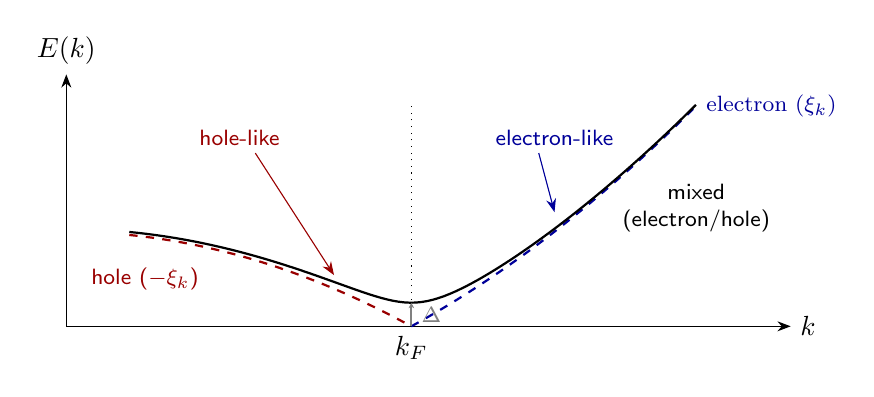
\begin{tikzpicture}[
    x=4.0cm, y=1.cm,
    >=Stealth,
    normal electron/.style={thick, dashed, blue!60!black},
    normal hole/.style={thick, dashed, red!60!black},
    sc/.style={thick, black},
    gap arrow/.style={thick, <->, gray},
    annotation/.style={font=\footnotesize\sffamily},
    pin text/.style={font=\footnotesize\sffamily},
]
\newcommand{\FermiEnergy}{1.2}          % µ
\newcommand{\GapValue}{0.3}             % Δ
\pgfmathsetmacro{\kF}{sqrt(\FermiEnergy)}  % k_F

% Axes
\draw[->] (0,0) -- (2.3,0) node[right] {$k$};
\draw[->] (0,0) -- (0,3.2) node[above] {$E(k)$};

% Fermi momentum marker
\draw[dotted, thin] (\kF,0) -- (\kF,2.8);
\node[below] at (\kF,0) {$k_F$};

% Normal-state electron branch (k > k_F)
\draw[normal electron, domain=\kF:2.0, samples=50]
    plot (\x, {\x*\x - \FermiEnergy})
    node[right, blue!60!black, font=\footnotesize] {electron ($\xi_k$)};

% Normal-state hole branch (k < k_F)
\draw[normal hole, domain=0.2:\kF, samples=50]
    plot (\x, {-\x*\x + \FermiEnergy});

% Superconducting branch (positive energy only)
\draw[sc, domain=0.2:2.0, samples=100]
    plot (\x, {sqrt((\x*\x - \FermiEnergy)^2 + \GapValue^2)});

% Gap arrow from zero to Δ
\draw[gap arrow, -{Stealth[length=2pt,width=2pt]}]
    (\kF,0) -- (\kF,\GapValue)
    node[midway,right,font=\footnotesize\sffamily] {$\Delta$};

\node[annotation, red!60!black] at (0.25,0.6) {hole ($-\xi_k$)};
% Annotations for the character of quasiparticles
\node[annotation, blue!60!black] at (1.55,2.4) {electron-like};
\draw[->, blue!60!black, thin] (1.5,2.2) -- (1.55,1.45);

\node[annotation, red!60!black] at (0.55,2.4) {hole-like};
\draw[->, red!60!black, thin] (0.6,2.2) -- (0.85,0.65);

\node[annotation, align=center] at (2.0,1.5) {mixed\\(electron/hole)};


\end{tikzpicture}
\caption{Energy spectrum of the normal state electron (blue dashed) and hole (red dashed), compared to the Bogoliubov quasiparticle dispersion (solid black).}
\label{fig:BdG_dispersion}
\end{figure}


    
\chapter{Tight-binding Bogoliubov-de Gennes equations}

In this chapter we reformulate the mean-field BCS theory on a lattice.  The tight-binding description is ideally suited for numerical simulations of inhomogeneous superconductors because it yields a finite-dimensional eigenvalue problem that can be solved self-consistently.  We first write down a general Hubbard Hamiltonian that includes on-site repulsion, inter-site attraction, and spin-dependent hopping.  After a mean-field decoupling in the pairing channel we obtain the Bogoliubov-de Gennes (BdG) equations in real space.  From these equations we derive the supercurrent operator, which will be used throughout the report to compute current-phase relations.

\section{Hubbard Hamiltonian on a lattice and mean-field decoupling}

We consider a set of atomic orbitals centered on the sites of a Bravais lattice.  Each orbital can accommodate at most two electrons (spin $\uparrow$ and $\downarrow$).  The Hamiltonian~\cite{zhu_bogoliubov-gennes_2016,micnas_superconductivity_1990} contains a single-particle (hopping) term and an on-site Coulomb interaction $U$:

\begin{equation}
  \hat{H} = \sum_{i,j}\sum_{\sigma,\sigma'} h_{i\sigma;j\sigma'} \, \hat{c}_{i\sigma}^\dagger \hat{c}_{j\sigma'}  + U \sum_i \hat{n}_{i\uparrow} \hat{n}_{i\downarrow},
    \label{eq:Hubbard}
\end{equation}
where $\hat{c}_{i\sigma}^\dagger$ creates an electron with spin $\sigma$ on site $i$, $\hat{n}_{i\sigma}=\hat{c}_{i\sigma}^\dagger\hat{c}_{i\sigma}$, and
\begin{equation}
  h_{i\sigma;j\sigma'} = \epsilon_i\,\delta_{ij}\delta_{\sigma\sigma'} - t_{i\sigma;j\sigma'} ,
  \qquad t_{i\sigma;i\sigma'}=0 .
\end{equation}
The diagonal term $\epsilon_i$ is the on-site energy, typically set to $-\mu$ (chemical potential).  The hopping amplitude $t_{i\sigma;j\sigma'}$ describes the probability for an electron to tunnel from site $j$ to site $i$. We assume spin-diagonal tunneling ($t_{i\sigma;j\sigma'}=t_{ij}\,\delta_{\sigma\sigma'}$).  The on-site $U$ is repulsive ($U>0$) in a normal metal but can be effectively negative when phonon-mediated attraction is included.


In the BCS theory, one assumes that the ground state has a finite anomalous average $\langle \hat{c}_{i\uparrow} \hat{c}_{j\downarrow}\rangle$. A quadratic effective Hamiltonian is obtained by replacing the four-fermion terms with all possible contractions of one pair of operators with respect to this ground state (Wick's theorem). Dropping the normal contractions (which would renormalize $h_{i\sigma;j\sigma'}$) and keeping only the anomalous ones gives
\begin{equation}
  \hat{n}_{i\uparrow}\hat{n}_{i\downarrow}
  = \hat{c}_{i\uparrow}^\dagger \hat{c}_{i\downarrow}^\dagger \hat{c}_{i\downarrow} \hat{c}_{i\uparrow}\approx  \langle\hat{c}_{i\uparrow}^\dagger \hat{c}_{i\downarrow}^\dagger\rangle\,
            \hat{c}_{i\downarrow} \hat{c}_{i\uparrow}
          + \hat{c}_{i\uparrow}^\dagger \hat{c}_{i\downarrow}^\dagger\,
            \langle\hat{c}_{i\downarrow} \hat{c}_{i\uparrow}\rangle
          - \langle\hat{c}_{i\uparrow}^\dagger \hat{c}_{i\downarrow}^\dagger\rangle\,
            \langle\hat{c}_{i\downarrow} \hat{c}_{i\uparrow}\rangle .
          \label{eq:dec_onsite}
\end{equation}


The anomalous averages define the pairing order parameters:
\begin{equation}
\boxed{
  \Delta_{i} \;=\; U \langle\hat{c}_{i\downarrow}\hat{c}_{i\uparrow}\rangle .
}
\label{eq:Delta_def_unified}
\end{equation}

Inserting the decoupling~\eqref{eq:dec_onsite} together with the definition~\eqref{eq:Delta_def_unified} into the original Hamiltonian~\eqref{eq:Hubbard} yields a quadratic effective Hamiltonian:

\begin{equation}
\boxed{
    \hat{H}_{\mathrm{MF}}^{\mathrm{s}} = \sum_{i,j}\sum_{\sigma,\sigma'} \widetilde{h}_{i\sigma;j\sigma'}\, \hat{c}_{i\sigma}^\dagger \hat{c}_{j\sigma'}
    + \sum_i \Bigl[ \Delta_i \hat{c}_{i\uparrow}^\dagger \hat{c}_{i\downarrow}^\dagger
    + \Delta_i^* \hat{c}_{i\downarrow} \hat{c}_{i\uparrow} \Bigr]\;+\; \text{const.}
}
\label{eq:H_MF_s-wave}
\end{equation}
Here \(\widetilde{h}_{i\sigma;j\sigma'}\) is the renormalized single-particle matrix. In practice these shifts simply renormalize the on-site energy and the chemical potential, so we can absorb them into a redefinition of \(\mu\).  We shall therefore write \(\widetilde{h}_{i\sigma;j\sigma'}=h_{i\sigma;j\sigma'}\) after this redefinition.



\section{Bogoliubov transformation and BdG equations}

In the absence of spin-orbit coupling the hopping is spin-diagonal and spin-independent, \(h_{i\uparrow;j\uparrow}=h_{i\downarrow;j\downarrow}=h_{ij}\), so the eigenstates are spin degenerate and the transformation to quasiparticle operators takes the form


\begin{align}
  \hat{c}_{i\uparrow} &= \sum_{n=1}^{N} \bigl[ u_{i}^{(n)} \hat{\gamma}_{n\uparrow} - v_{i}^{(n)*} \hat{\gamma}_{n\downarrow}^\dagger \bigr], \label{eq:trafo_up_simple} \\
  \hat{c}_{i\downarrow} &= \sum_{n=1}^{N} \bigl[ u_{i}^{(n)} \hat{\gamma}_{n\downarrow} + v_{i}^{(n)*} \hat{\gamma}_{n\uparrow}^\dagger \bigr]. \label{eq:trafo_down_simple}
\end{align}

The quasiparticle operators must satisfy the canonical fermionic anti-commutation relations.  Substituting the transformation~\eqref{eq:trafo_up_simple}-\eqref{eq:trafo_down_simple} into \(\{\hat{c}_{i\sigma},\hat{c}_{j\sigma'}^\dagger\}=\delta_{ij}\delta_{\sigma\sigma'}\) and \(\{\hat{c}_{i\sigma},\hat{c}_{j\sigma'}\}=0\) yields the following completeness and orthogonality constraints on the amplitudes:
\begin{align}
  \sum_{n=1}^{N} \bigl( u_{i}^{(n)} u_{j}^{(n)*} + v_{i}^{(n)*} v_{j}^{(n)} \bigr) &= \delta_{ij}, \label{eq:completeness1} \\
  \sum_{n=1}^{N} \bigl( u_{i}^{(n)} v_{j}^{(n)*} - v_{i}^{(n)*} u_{j}^{(n)} \bigr) &= 0, \label{eq:ortho1} \\
  \sum_{i=1}^{N} \bigl( u_{i}^{(n)*} u_{i}^{(m)} + v_{i}^{(n)*} v_{i}^{(m)} \bigr) &= \delta_{nm}\quad\text{by orthonormality of the eigenvectors.}\label{eq:ortho2}
\end{align}


Requiring that the Bogoliubov transformation~\eqref{eq:trafo_up_simple}-\eqref{eq:trafo_down_simple} brings the mean-field Hamiltonian~\eqref{eq:H_MF_s-wave} to the diagonal form
\begin{equation}
  \hat{H}_{\mathrm{MF}}^{\mathrm{s}} = E_g + \sum_{n,\sigma} E_{n} \hat{\gamma}_{n\sigma}^\dagger \hat{\gamma}_{n\sigma},
  \label{eq:H_diag_swave}
\end{equation}
yields the Bogoliubov-de Gennes (BdG) equations
\begin{equation}
  \boxed{
  \begin{aligned}
    E_{n} u_{i}^{(n)} &= \sum_{j} h_{ij} u_{j}^{(n)} + \Delta_{i} v_{i}^{(n)}, \\
    E_{n} v_{i}^{(n)} &= -\sum_{j} h_{ij}^{*} v_{j}^{(n)} + \Delta_{i}^{*} u_{i}^{(n)}.
  \end{aligned}
  }
  \label{eq:BdG_swave}
\end{equation}
These equations can be written as a matrix eigenvalue problem of dimension \(2N\):
\begin{equation}
  \sum_{j=1}^{N} \mathcal{H}_{ij}
  \begin{pmatrix} u_{j}^{(n)} \\[2pt] v_{j}^{(n)} \end{pmatrix}
  = E_{n} \begin{pmatrix} u_{i}^{(n)} \\[2pt] v_{i}^{(n)} \end{pmatrix},
  \qquad
  \mathcal{H}_{ij} =
  \begin{pmatrix}
    h_{ij} & \Delta_{i}\,\delta_{ij} \\[4pt]
    \Delta_{i}^{*}\,\delta_{ij} & -h_{ij}^{*}
  \end{pmatrix}.
  \label{eq:M_swave}
\end{equation}

\section{Particle-hole symmetry}

An important property of the BdG equations is particle-hole symmetry: if \((u_i^{(n)},v_i^{(n)})^{\mathsf T}\) is an eigenvector with energy \(E_n\), then
\begin{equation}
  \begin{pmatrix} u_i^{(-n)} \\[2pt] v_i^{(-n)} \end{pmatrix}
  = \begin{pmatrix} v_i^{(n)*} \\[2pt] -u_i^{(n)*} \end{pmatrix}
  \label{eq:ph_symmetry}
\end{equation}
is an eigenvector with energy \(-E_n\).  This symmetry doubles the number of solutions. Physically, the \(n>0\) states describe quasiparticle excitations while the \(n<0\) states are their hole counterparts.

The physical content of this symmetry is revealed by the explicit form of the quasiparticle operators.  According to the inverse transformation
\begin{equation}
  \hat{\gamma}_{n\uparrow} \;=\; \sum_i \bigl( u_i^{(n)*} \hat{c}_{i\uparrow} + v_i^{(n)*} \hat{c}_{i\downarrow}^\dagger \bigr),\qquad\hat{\gamma}_{n\downarrow} = \sum_i \bigl( u_i^{(n)*} \hat{c}_{i\downarrow} -v_i^{(n)*} \hat{c}_{i\uparrow}^\dagger \bigr).
  \label{eq:gamma_n}
\end{equation}
For the negative-energy partner (labeled by \(-n\)), we insert the amplitudes~\eqref{eq:ph_symmetry} into the same formula. We obtain
\begin{equation}
  \boxed{\;\hat{\gamma}_{-n,\uparrow} \;=\; -\,\hat{\gamma}_{n,\downarrow}^\dagger,\;\qquad\;\hat{\gamma}_{-n,\downarrow} \;=\; \hat{\gamma}_{n,\uparrow}^\dagger\;}.
  \label{eq:relation_up_down}
\end{equation}

Equations~\eqref{eq:relation_up_down} show that the negative-energy quasiparticle operators are not independent degrees of freedom. They are the creation operators of the positive-energy quasiparticles. Creating a hole in the Fermi sea is equivalent to annihilating a particle of opposite spin.

Consequently, only the $N$ eigenstates with positive energy \(E_n>0\) are needed to describe all physical excitations.  The diagonalized Hamiltonian can therefore be written exclusively in terms of the positive-energy branch.










\section{Self-consistent gap equation}
\label{sec:self consistent gap eq}
The order parameter must be evaluated self-consistently from the definition \(\Delta_{i} = U\langle \hat{c}_{i\downarrow} \hat{c}_{i\uparrow}\rangle\). Using the transformation~\eqref{eq:trafo_up_simple}-\eqref{eq:trafo_down_simple} and the fermionic thermal averages, we obtain,
\begin{equation}
  \boxed{
    \Delta_{i} = -U \sum_{n=1}^N u_{i}^{(n)} v_{i}^{(n)*} \,
                \tanh\!\left( \frac{\beta E_{n}}{2} \right) .
  }
  \label{eq:Delta_sum_all}
\end{equation}

Using the particle-hole pairing, the sum over the $N$ positive energies can be recast as a symmetric sum over all $2N$ eigenstates,
\begin{equation}
  \boxed{
    \Delta_{i} = -\,\frac{U}{2} \sum_{n} u_{i}^{(n)} v_{i}^{(n)*} \,
                \tanh\!\left( \frac{\beta E_{n}}{2} \right) .
  }
  \label{eq:gap_equation_final}
\end{equation}


It can be shown that this is equivalent to extremizing the free energy of the system.




\section{Supercurrent}

The current in a tight-binding lattice is obtained from the continuity equation $i\hbar\,\partial_t  \hat{n}_i = [\hat{n}_i,\hat{H}]$ for the site occupation \(\hat{n}_i = \sum_{\sigma} \hat{c}_{i\sigma}^\dagger \hat{c}_{i\sigma}\). The current from site \(j\) to site \(i\) is
\begin{equation}
  \hat{J}_{j\to i} = -e\,\frac{\partial \hat{n}_i}{\partial t}\Big|_{j\to i}
  = \frac{ie}{\hbar} \sum_{\sigma}\left[t_{ji}\hat{c}_{j\sigma}^\dagger\hat{c}_{i\sigma}-t_{ij} \hat{c}_{i\sigma}^\dagger\hat{c}_{j\sigma}\right].
  \label{eq:J_op}
\end{equation}
Taking the thermal expectation value and inserting the Bogoliubov transformation yields the Josephson current

\begin{equation}
  \boxed{
    J_{j\to i} = \frac{2e}{\hbar}\,
    \mathrm{Im}\!\left(t_{ij}\,
      \sum_{n} \bigl[ u_{i}^{(n)*} u_{j}^{(n)} n_F(E_n)
                    + v_{i}^{(n)} v_{j}^{(n)*} n_F(-E_n) \bigr]
    \right) .
  }
  \label{eq:J_final}
\end{equation}

\chapter{Uniform s-wave superconductor: Phase diagram and finite-size effects}

In this chapter we apply the s-wave BdG formalism of the previous chapter to a homogeneous, translationally invariant superconductor.  We derive the analytical quasiparticle spectrum and the self-consistent gap equation, and we compare the predictions with exact numerical diagonalization of a finite chain.


\section{Translationally invariant solutions}

We consider a tight-binding lattice with nearest-neighbor hopping \(t\) and on-site energy \(-\mu\). In a uniform superconductor the order parameter is site-independent, \(\Delta_i \equiv \Delta\).  Because of translational invariance, the BdG wavefunctions satisfy Bloch's theorem,
\begin{equation}
  u_i^{(n)} = \frac{1}{\sqrt{N}}\,u_{k}\,e^{\mathrm{i} k R_i} ,\qquad
  v_i^{(n)} = \frac{1}{\sqrt{N}}\,v_{k}\,e^{\mathrm{i} k R_i} ,\qquad |u_{k}|^{2}+|v_{k}|^{2}=1,
\end{equation}
where the lattice momentum \(k\) ($k_x$ and $k_y$ in 2D) takes values \(
k = \frac{2\pi m}{N a}\) with \(m=0,1,\dots,N-1,\) for a finite chain with periodic boundary conditions, or runs continuously over the first Brillouin zone \([0,2\pi/a)\) in the thermodynamic limit \(N\to\infty\).

Inserting the Bloch ansatz into the BdG eigenvalue equation~\eqref{eq:M_swave} yields the reduced problem
\begin{equation}
  \begin{pmatrix}
    \xi_{\mathbf{k}} & \Delta \\[2pt]
    \Delta^{*} & -\xi_{\mathbf{k}}
  \end{pmatrix}
  \begin{pmatrix}
    u_{\mathbf{k}} \\[2pt] v_{\mathbf{k}}
  \end{pmatrix}
  = E_{\mathbf{k}}
  \begin{pmatrix}
    u_{\mathbf{k}} \\[2pt] v_{\mathbf{k}}
  \end{pmatrix},
\end{equation}
yielding the BCS dispersion and the condition
\begin{equation}
  E_{\mathbf{k}} = \pm\sqrt{\xi_{\mathbf{k}}^{2}+|\Delta|^{2}} ,\qquad
    u_{\mathbf{k}}  v_{\mathbf{k}}^*=\frac{\Delta}{2E_{\mathbf{k}}}.
\end{equation}
The single-particle dispersion is $\xi_{\mathbf{k}}=\sum_jh_{ij}e^{\mathrm{i}\mathbf{k}\cdot(\mathbf{R}_j-\mathbf{R}_i)}$, which evaluates to
\begin{align}
  \xi_{k} &= -\mu - 2t\cos(ka)  &&(d=1), \\
  \xi_{\mathbf{k}} &= -\mu - 2t(\cos k_x a + \cos k_y a) &&(d=2).
\end{align}

The self-consistency condition~\eqref{eq:gap_equation_final} then becomes 
\begin{equation}
  \boxed{
  1 = -\frac{U}{2N}\sum_{\mathbf{k}} \frac{1}{E_{\mathbf{k}}} \tanh\!\left(\frac{E_{\mathbf{k}}}{2k_{B}T}\right) ,
  }
  \label{eq:gap_1D}
\end{equation}
where the sum runs over the \(N\) allowed momentum states. In the thermodynamic limit, the momentum sum is replaced by an integral over the first Brillouin zone:
\begin{equation}
    \boxed{
    1 = -\frac{U}{2}\,\frac{a^{d}}{(2\pi)^{d}} \int_{\mathrm{BZ}} \! d^{d}k\;
    \frac{1}{E_{\mathbf{k}}}
    \tanh\!\left(\frac{E_{\mathbf{k}}}{2k_{B}T}\right)
    ,}
  \label{eq:gap_gen}
\end{equation}
where \(d=1,2\) is the spatial dimension.  Equation~\eqref{eq:gap_gen} determines \(\Delta(T)\) and the critical temperature \(T_c\) (where \(\Delta\to0\)). The critical temperature \(T_c(\mu)\) is the temperature at which the self-consistent order parameter vanishes. It is obtained by setting \(\Delta=0\) in the integral equation:
\begin{align}
  -\frac{U}{4\pi}\int_{0}^{2\pi} \frac{\mathrm{d}\theta}{|\mu+2t\cos\theta|}\,
  \tanh\!\left(\frac{|\mu+2t\cos\theta|}{2k_{B}T_c}\right) &= 1 , \qquad (\theta=ka)
  \label{eq:Tc_1D} \\[6pt]
  -\frac{U}{8\pi^{2}} \int_{0}^{2\pi}\!\!\!\int_{0}^{2\pi}\!\! \frac{\mathrm{d}\theta_x\mathrm{d}\theta_y}
  {|\mu+2t(\cos\theta_x+\cos\theta_y)|}\,
  \tanh\!\left(\frac{|\mu+2t(\cos\theta_x+\cos\theta_y)|}{2k_{B}T_c}\right) &= 1 ,
  \label{eq:Tc_2D}
\end{align}
for \(d=1\) and \(d=2\), respectively.






\section{Phase diagrams and order parameter}

We solve the integral equations~\eqref{eq:Tc_1D} and~\eqref{eq:Tc_2D} numerically for \(T_c\) as a function of \(\mu\).  The results are shown in Figure~\ref{fig:Tc_vs_mu}.


\begin{figure}[H]
  \centering
  \begin{subfigure}[b]{0.48\textwidth}
    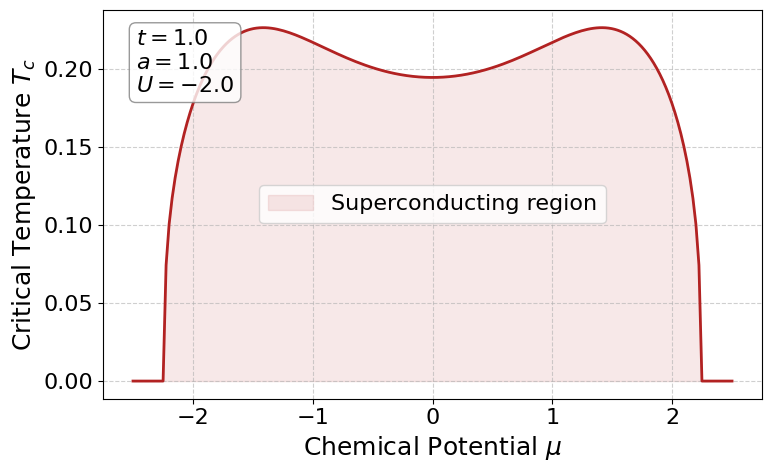
\includegraphics[width=\textwidth]{figures/ch4_tc_vs_mu_1d.png}
    \caption{1D}
    \label{fig:phase_diag_1D}
  \end{subfigure}
  \hfill
  \begin{subfigure}[b]{0.48\textwidth}
    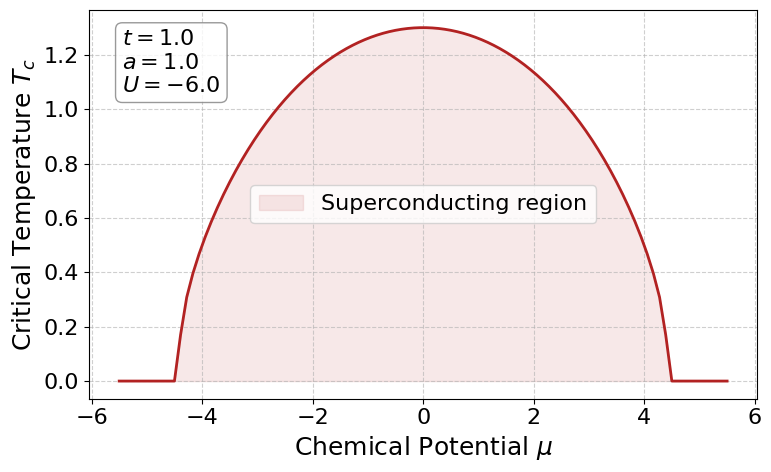
\includegraphics[width=\textwidth]{figures/ch4_tc_vs_mu_2d.png}
    \caption{2D}
    \label{fig:phase_diag_2D}
  \end{subfigure}
  \caption{Critical temperature as a function of chemical potential.}
  \label{fig:Tc_vs_mu}
\end{figure}


The critical temperature \(T_c(\mu)\) is obtained by setting \(\Delta=0\) in the gap equation.  For the 1D case this yields
\begin{equation}
-\frac{U a}{4\pi}\int_{0}^{2\pi/a}\!\!dk\;
\frac{1}{|\xi_k|}\,\tanh\!\left(\frac{|\xi_k|}{2k_{B}T_c}\right)=1 ,
\label{eq:Tc_1D_k}
\end{equation}
where \(\xi_k = -\mu-2t\cos(ka)\). Since the integrand depends on \(k\) only through \(\xi_k\), we transform the integral
to an energy integral.  In the interval \(k\in[0,\pi/a]\) the function \(\xi_k\) is monotonic, and the whole Brillouin zone
is covered twice. Hence
\[
\int_{0}^{2\pi/a}\!\!dk \;\longrightarrow\; 2\int_{\xi_{\min}}^{\xi_{\max}} \frac{d\xi}{|d\xi/dk|}.
\]
The density of states is defined as
\[
g(\xi) = \frac{1}{|d\xi/dk|} = \frac{1}{2ta|\sin(ka)|},\qquad
\xi = -\mu-2t\cos(ka) .
\]
Explicitly,
\[
g(\xi) = \frac{1}{2 t a}\,\frac{1}{\sqrt{1-(\xi+\mu)^2/4t^2}},\qquad |\xi+\mu|\leq 2t .
\]
Substituting the transformation into~\eqref{eq:Tc_1D_k} we obtain
\begin{equation}
-\frac{U a}{2\pi}\int_{-2t-\mu}^{2t-\mu}\!\!d\xi\;
\frac{g(\xi)}{|\xi|}\,\tanh\!\left(\frac{|\xi|}{2k_{B}T_c}\right)=1 .
\label{eq:Tc_1D_DOS}
\end{equation}

The peak of \(g(\xi)\) always lies at the integration limits, but its contribution to the integral is controlled by the factor \(1/|\xi|\). This factor strongly suppresses energies far from the Fermi level (\(\xi=0\)). When the chemical potential is near a band edge (\(|\mu|\approx 2t\)), the Fermi level itself approaches the Van Hove singularity, and the peaks of \(g(\xi)\) and \(1/|\xi|\) coincide. The integral then becomes large, and \(T_c\) must rise to satisfy the equation. Conversely, when \(\mu\approx 0\), the Fermi level sits at the band center where the DOS is moderate, and the singularities, though present, are at the integration limits where \(1/|\xi|\) is small, contributing little.  The maximum of \(T_c\) therefore occurs at an intermediate value of \(\mu\) where the two competing effects, the DOS enhancement near the band edges and the \(1/|\xi|\) peak at the Fermi level, are balanced. In 1D this leads to an off-center dome.
  


In two dimensions, the DOS exhibits a logarithmic Van Hove singularity at the band center (\(\mu=0\)). The corresponding energy integral then peaks at \(\mu=0\), yielding the familiar dome-shaped phase boundary.


\subsection{Critical behavior near $T_c$}

Just below the critical temperature, the order parameter is small, \(\Delta(T)\ll k_B T_c\), and the gap equation can be expanded to obtain the power law with which \(\Delta\) vanishes.  We start from the thermodynamic limit equation~\eqref{eq:gap_gen}
\[
1 = -\frac{U}{2} \int_{\mathrm{BZ}}\!\frac{\mathrm{d}^{d}k}{(2\pi)^{d}}\;
\frac{1}{E_{\mathbf{k}}}\,\tanh\!\left(\frac{E_{\mathbf{k}}}{2k_B T}\right),
\qquad E_{\mathbf{k}}=\sqrt{\xi_{\mathbf{k}}^2+|\Delta|^2}.
\]
At \(T=T_c\) we have \(\Delta=0\), therefore
\[
1 = -\frac{U}{2} \int_{\mathrm{BZ}}\!\frac{\mathrm{d}^{d}k}{(2\pi)^{d}}\;
\frac{1}{|\xi_{\mathbf{k}}|}\,\tanh\!\left(\frac{|\xi_{\mathbf{k}}|}{2k_B T_c}\right).
\]
Subtracting the two equations gives
\[
0 = -\frac{U}{2} \int_{\mathrm{BZ}}\!\frac{\mathrm{d}^{d}k}{(2\pi)^{d}}\;
\left[ \frac{1}{E_{\mathbf{k}}}\tanh\!\left(\frac{E_{\mathbf{k}}}{2k_B T}\right) -
\frac{1}{|\xi_{\mathbf{k}}|}\tanh\!\left(\frac{|\xi_{\mathbf{k}}|}{2k_B T_c}\right) \right].
\]
For temperatures \(T\) close to \(T_c\) we expand the integrand in powers of the small quantities \(|\Delta|^2\) and \(\delta T=T_c-T\),
\begin{align}
\frac{1}{E}\tanh\!\left(\frac{E}{2k_B T}\right) &\approx
\frac{1}{|\xi|}\tanh\!\left(\frac{|\xi|}{2k_B T_c}\right)
+ |\Delta|^2 \,\frac{\partial}{\partial|\Delta|^2}\!\left[ \frac{1}{E}\tanh\!\left(\frac{E}{2k_B T_c}\right)\right]_{\Delta=0}\notag\\
&+ (T-T_c)\,\frac{\partial}{\partial T}\!\left[ \frac{1}{|\xi|}\tanh\!\left(\frac{|\xi|}{2k_B T}\right)\right]_{T=T_c}.
\end{align}
Inserting this expansion into the subtracted gap equation, we get
\begin{align*}
&|\Delta|^2 \int_{\mathrm{BZ}}\!\frac{\mathrm{d}^{d}k}{(2\pi)^{d}}\,
\frac{1}{2|\xi|^3}\left[ \frac{|\xi|}{2k_B T_c}\operatorname{sech}^2\!\left(\frac{|\xi|}{2k_B T_c}\right) - \tanh\!\left(\frac{|\xi|}{2k_B T_c}\right) \right] \nonumber\\
&\qquad + (T-T_c)\int_{\mathrm{BZ}}\!\frac{\mathrm{d}^{d}k}{(2\pi)^{d}}\,
\left( -\frac{1}{2k_B T_c^2}\,\operatorname{sech}^2\!\left(\frac{|\xi|}{2k_B T_c}\right) \right) = 0 . \label{eq:expanded}
\end{align*}
Both integrals converge.  For the first, the bracket vanishes as $\xi\to0$:
\[
\frac{|\xi|}{2k_B T_c}\operatorname{sech}^2\!\left(\frac{|\xi|}{2k_B T_c}\right) - \tanh\!\left(\frac{|\xi|}{2k_B T_c}\right)
= -\frac{2}{3}\left(\frac{|\xi|}{2k_B T_c}\right)^3 + O(|\xi|^5),
\]
which cancels the $1/|\xi|^3$ prefactor, leaving a finite integrand. The second integral contains no singularity. Consequently one obtains
\[
\Delta^2 \;\propto\; T_c - T ,
\]
so that for \(T\lesssim T_c\)
\[
\boxed{\;\Delta(T) \approx A\; \left(1-\frac{T}{T_c}\right)^{1/2}\;}.
\]
The critical exponent \(\alpha = 1/2\) is universal for all dimensions. This behavior is clearly visible in the numerical solutions shown in Fig.~\ref{fig:Delta_vs_T}, where \(\Delta(T)\) vanishes with a vertical slope at \(T_c\).

\begin{figure}[H]
  \centering
  \begin{subfigure}[b]{0.48\textwidth}
    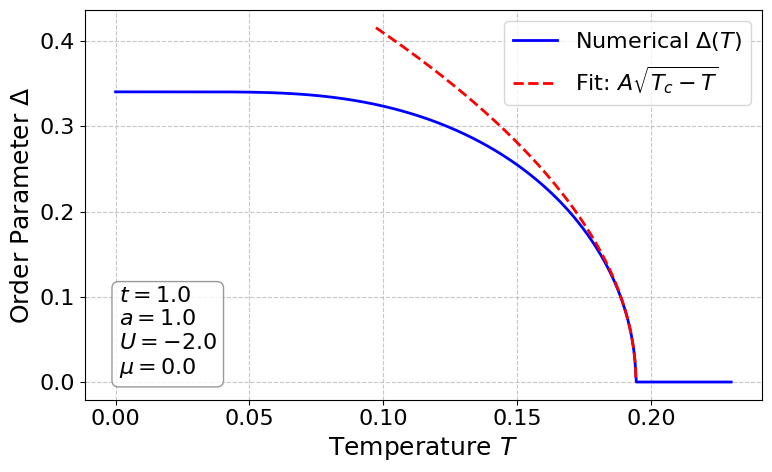
\includegraphics[width=\textwidth]{figures/ch4_gap_vs_temperature_1d.png}
    \caption{1D}
    \label{fig:Delta_vs_T_1D}
  \end{subfigure}
  \hfill
  \begin{subfigure}[b]{0.48\textwidth}
    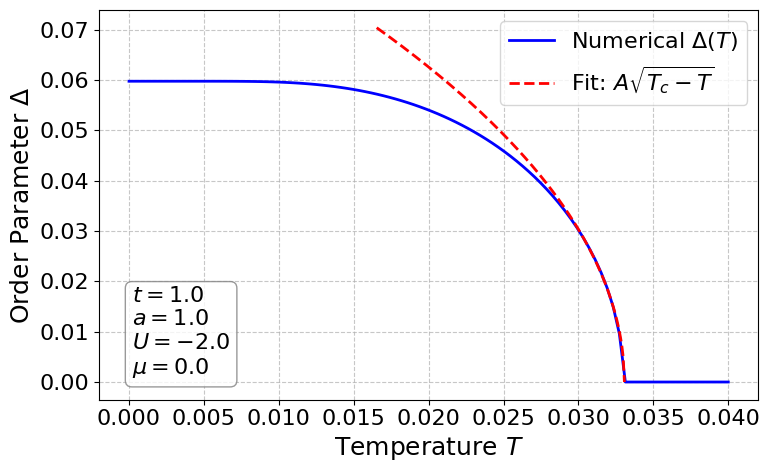
\includegraphics[width=\textwidth]{figures/ch4_gap_vs_temperature_2d.png}
    \caption{2D}
    \label{fig:Delta_vs_T_2D}
  \end{subfigure}
  \caption{Magnitude of the self-consistent order parameter as a function of temperature.}
  \label{fig:Delta_vs_T}
\end{figure}

\section{Finite-size convergence}

To verify that our numerical methods faithfully reproduce the thermodynamic limit, we compare three different approaches to solving the gap equation for a 1D chain: a finite chain with open boundary conditions, a finite chain with periodic boundary conditions, and the thermodynamic limit where the sum is replaced by the integral~\eqref{eq:gap_gen}.  In each case we compute the order parameter \(\Delta\) self-consistently for a given chain length \(N\) and compare it with the thermodynamic limit value.


\begin{figure}[H]
    \centering
    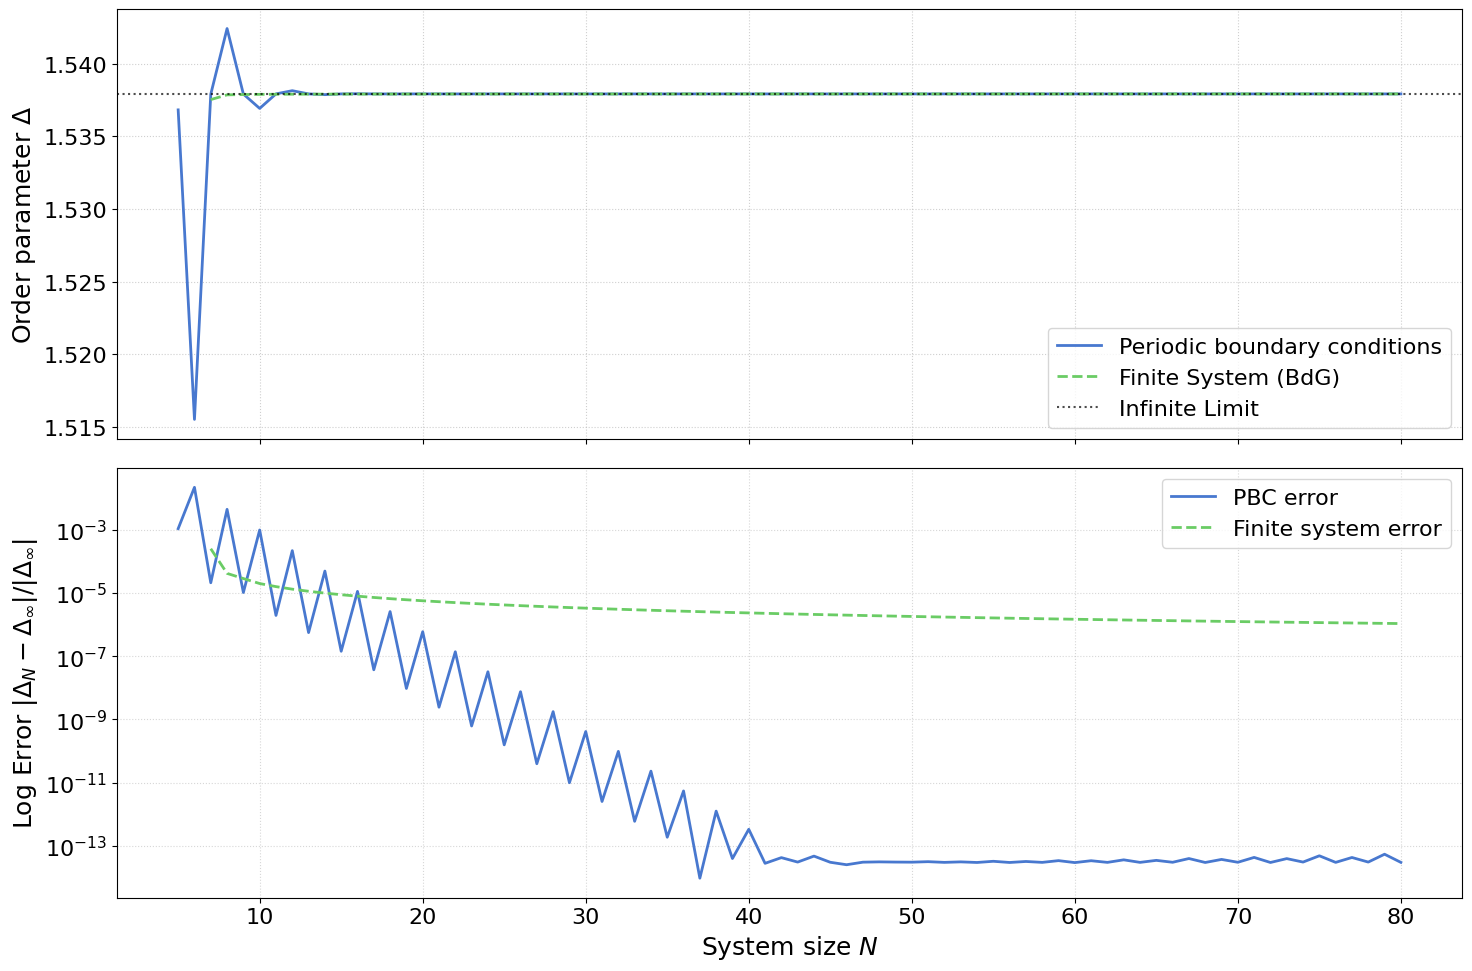
\includegraphics[width=0.7\textwidth]{figures/ch4_finite_size_convergence.png}
    \caption{Order parameter \(\Delta\) as a function of chain length \(N\) for a 1D chain.}
  \label{fig:Delta_vs_N}
\end{figure}





The three approaches converge to the same value as \(N\) increases. For \(N\gtrsim 15\) the relative error with respect to the thermodynamic limit is already below \(10^{-5}\). This rapid convergence justifies the use of moderate chain lengths throughout the rest of this work.





\chapter{Josephson junctions: concepts, modeling, and self-consistent calculations}

\section{Concept and applications of Josephson junction}

The Josephson effect, predicted by Brian Josephson in 1962~\cite{josephson_possible_1962}, describes the situation in which two superconductors are separated by a weak link (a thin insulating barrier, a normal metal, or a narrow constriction), a dissipationless supercurrent can flow between them even in the absence of a voltage.  This current is a periodic function of the phase difference \(\phi = \phi_R - \phi_L\) between the two superconductors. For a tunnel junction, it holds that:
\begin{equation}
  I(\phi) = I_{\max} \sin\phi.
\end{equation}
The amplitude \(I_{\max}\) (the critical current) depends on the properties of the weak link and on temperature.

Josephson junctions are the building blocks of superconducting electronics.  They are used in:
\begin{itemize}
    \item \textbf{SQUIDs} (Superconducting QUantum Interference Devices) are extremely sensitive magnetometers built from a superconducting loop interrupted by one (rf-SQUID) or two (dc-SQUID) Josephson junctions. In a dc-SQUID, a bias current is passed through the two parallel junctions. The phase difference around the loop is directly proportional to the magnetic flux threading it, so the critical current of the parallel pair modulates periodically with the external flux, as illustrated in Fig.~\ref{fig:squid}. By biasing the SQUID slightly above its critical current and measuring the voltage drop, one can detect flux of the order of \(10^{-6}\,\Phi_0/\sqrt{\text{Hz}}\) (where \(\Phi_0 = h/2e\)). This extraordinary sensitivity has enabled applications ranging from magnetoencephalography (MEG) which maps neuronal brain currents with millisecond temporal and millimeter spatial resolution, to low-field MRI, airborne geophysical surveys for mineral exploration, fundamental physics research areas (magnetic monopoles, axion dark matter, precision tests of quantum electrodynamics), and materials characterization (e.g., MPMS systems).~\cite{clarke_squid_2004}.
        \begin{figure}[H]
        \centering
        \begin{minipage}[c]{0.45\textwidth}
        \centering
        \begin{circuitikz}[scale=0.9, transform shape]
          % ----- Top and bottom rails -----
          \draw (0,2) to[short,-] (3,2);   % top rail
          \draw (0,0) to[short,-] (3,0);   % bottom rail
        
          % ----- Left Josephson junction J1 -----
          \node[draw, minimum width=0.7cm, minimum height=0.7cm] (J1) at (0,1) {};
          \draw (J1.north west) -- (J1.south east);
          \draw (J1.north east) -- (J1.south west);
          \draw (J1.north) to[short] ++(0,0.5) coordinate (tmp) -- (0,2);
          \draw (J1.south) to[short] ++(0,-0.5) -- (0,0);
          \node at (J1.west) [left=1mm] {$J_1$};
        
          % ----- Right Josephson junction J2 -----
          \node[draw, minimum width=0.7cm, minimum height=0.7cm] (J2) at (3,1) {};
          \draw (J2.north west) -- (J2.south east);
          \draw (J2.north east) -- (J2.south west);
          \draw (J2.north) -- ++(0,0.5) -- (3,2);
          \draw (J2.south) -- ++(0,-0.5) -- (3,0);
          \node at (J2.east) [right=1mm] {$J_2$};
        
          % ----- Bias current leads -----
          \draw (1.5,0) to[short, *-] (1.5,-0.8) node[below] {$I_{\mathrm{bias}}$};
          \draw (1.5,2) to[short, *-] (1.5,2.8);  % (top lead, unused)
        
          \node[circle, draw, inner sep=0pt, minimum size=4mm] at (1.5,1) {};
          \node at (1.5,1) {$\cdot$};   % central dot → flux out of page
          \node[blue] at (1.8,0.6) {$\Phi$};
          \node[blue] at (4,-0.7) [above] {$\Phi_0 = h/2e$};
            
        \end{circuitikz}
        \subcaption{dc-SQUID circuit.}
        \label{fig:squid_circuit}
        \end{minipage}
        \hfill
        \begin{minipage}[c]{0.52\textwidth}
        \centering
        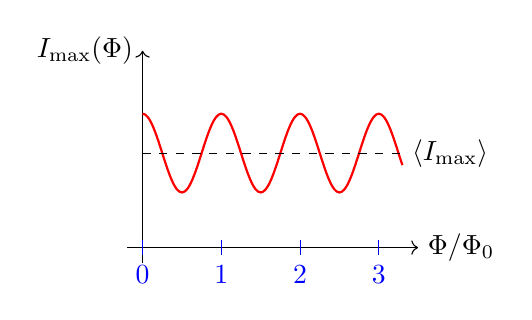
\begin{tikzpicture}[scale=1.0]
          % Axes
          \draw[->] (-0.2,0) -- (3.5,0) node[right] {$\Phi/\Phi_0$};
          \draw[->] (0,-0.2) -- (0,2.5) node[left] {$I_{\max}(\Phi)$};
        
          % Critical current oscillation
          \draw[domain=0:3.3, samples=100, smooth, thick, red]
            plot (\x, {1.2 + 0.5*cos(360*\x)});
          \draw[dashed] (0,1.2) -- (3.3,1.2) node[right] {$\langle I_{\max} \rangle$};
        
          % Period markers
          \foreach \x/\l in {0/0, 1/1, 2/2, 3/3} {
            \draw[blue] (\x,0.1) -- (\x,-0.1) node[below] {$\l$};
          }
        \end{tikzpicture}
        \subcaption{Critical current vs. flux: $I_{\max}$ oscillates with period $\Phi_0$.}
        \label{fig:squid_modulation}
        \end{minipage}
        \caption{dc-SQUID principle.}
        \label{fig:squid}
        \end{figure}
    \item \textbf{Voltage standards} derived from large series arrays of Josephson junctions constitute the international standard for the Volt, as they deliver a voltage that is precisely linked to the microwave frequency and the flux quantum \(\Phi_0\).~\cite{hamilton_josephson_1997}.
   \item \textbf{Quantum bits} (qubits) require a well-isolated two-level system whose states can be selectively addressed without inadvertently populating higher levels. A pure superconducting LC oscillator is a harmonic system with energy levels equally spaced, so a microwave drive resonant with the \(|0\rangle\!\to\!|1\rangle\) transition also excites \(|1\rangle\!\to\!|2\rangle\), \(|2\rangle\!\to\!|3\rangle\), etc., and the dynamics cannot be confined to two levels. The Josephson junction solves this problem by modifying the potential energy of the circuit from a simple parabola (\(U\propto\Phi^{2}\)) to an anharmonic shape \(U(\varphi)=-E_J\cos\varphi\) (where \(\varphi=2\pi\Phi/\Phi_0\) is the phase difference across the junction), as depicted in Fig.~\ref{fig:qubit_principles}. This anharmonicity makes the transition frequencies unequal, with \(\omega_{01}\neq\omega_{12}\neq\omega_{23}\ldots\). By tuning a microwave pulse to \(\omega_{01}\), one can drive the \(|0\rangle\leftrightarrow|1\rangle\) transition without ever populating higher states. The system behaves as an effective two-level qubit. The quantum variable is the phase of the circuit and its wavefunction \(\psi(\Phi)\) describes the probability amplitude for measuring a given flux, and the qubit can be prepared in superpositions of the
  ground (\(|0\rangle\)) and excited (\(|1\rangle\)) energy eigenstates.~\cite{devoret2013superconducting}.

\end{itemize}



\begin{figure}[H]
\centering
\begin{subfigure}[b]{0.4\textwidth}
    \centering
    \begin{circuitikz}[scale=1.0, transform shape]
      % Top and bottom rails
      \draw (0,2) to[short,*-] (3.5,2);
      \draw (0,0) to[short,*-] (3.5,0);

      % Left branch: capacitor
      \draw (0.5,2) to[C, l=$C$] (0.5,0);

      % Middle branch: custom Josephson junction
      \coordinate (JJtop) at (2,2);
      \coordinate (JJbot) at (2,0);
      \node[draw, minimum width=0.7cm, minimum height=0.7cm] (JJ) at (2,1) {};
      \draw (JJ.north west) -- (JJ.south east);
      \draw (JJ.north east) -- (JJ.south west);
      \draw (JJtop) -- (JJ.north);
      \draw (JJ.south) -- (JJbot);
      \node at (JJ.east) [right=1mm] {$E_J$};

      % Right branch: inductor
      \draw (3.5,2) to[L, l=$L$] (3.5,0);

      % Flux arrow
      \draw[->, thick] (4.3,0.5) -- node[midway,right] {$\varphi = \frac{2\pi}{\Phi_0}\Phi$} (4.3,1.5);
    \end{circuitikz}
    \caption{Superconducting qubit circuit with Josephson junction, capacitor and inductor.}
    \label{fig:qubit_circuit_clean}
\end{subfigure}
\hspace{1cm}
\begin{subfigure}[b]{0.4\textwidth}
    \centering
    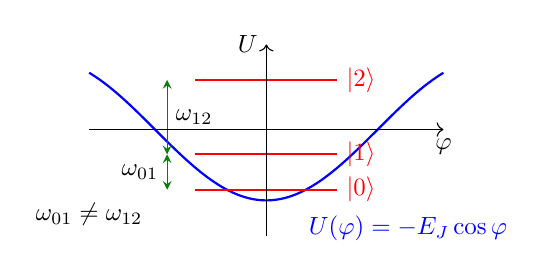
\begin{tikzpicture}[scale=0.9, transform shape]
    % Potential energy curve
    \draw[domain=-2.5:2.5,samples=100,smooth,variable=\x,blue,thick]
      plot (\x,{-cos(\x r)});
    \node[blue] at (2.0,-1.4) {$U(\varphi) = -E_J\cos\varphi$};

    % Energy levels
    \draw[red,thick] (-1.0, -0.85) -- (1.0, -0.85) node[right] {$\ket{0}$};
    \draw[red,thick] (-1.0, -0.35) -- (1.0, -0.35) node[right] {$\ket{1}$};
    \draw[red,thick] (-1.0, +0.70) -- (1.0, +0.70) node[right] {$\ket{2}$};

    % Transition frequencies
    \draw[<->,>=stealth,green!50!black] (-1.4,-0.85) -- (-1.4,-0.35)
      node[midway,left,black] {$\omega_{01}$};
    \draw[<->,>=stealth,green!50!black] (-1.4,-0.35) -- (-1.4,0.70)
      node[midway,right,black] {$\omega_{12}$};

    \node at (-2.5,-1.2) {$\omega_{01}\neq\omega_{12}$};

    % Axes
    \draw[->] (-2.5,0) -- (2.5,0) node[below] {$\varphi$};
    \draw[->] (0,-1.5) -- (0,1.2) node[left] {$U$};
    \draw[dotted] (-2.5,0) -- (2.5,0);
    \end{tikzpicture}
    \caption{Anharmonic potential with the three lowest energy eigenstates.}
    \label{fig:anharmonic_potential_combined}
\end{subfigure}
\caption{Superconducting qubit principles.}
\label{fig:qubit_principles}
\end{figure}






There exist different types of Josephson junctions, each realized by a distinct weak link between two superconductors:
\begin{itemize}
  \item \textbf{SIS} (Superconductor-Insulator-Superconductor): The link is a thin insulating tunnel barrier (typically $1$-$2\,\text{nm}$ of aluminium oxide). Cooper pairs tunnel through the barrier, giving a sinusoidal current-phase relation \(I(\phi) = I_{\max}\sin\phi\) with a critical current determined by the junction’s normal-state resistance and the superconducting gap.
  
  \item \textbf{SNS} (Superconductor-Normal metal-Superconductor): The link is a non-superconducting (normal) metal layer of length \(L\) connecting the two superconductors. The normal region hosts Andreev bound states that carry the supercurrent.
  
  \item \textbf{ScS} (Superconductor-constriction-Superconductor) or \textbf{microbridge}: The two superconductors are linked by a narrow superconducting neck whose dimensions are comparable to the coherence length.
\end{itemize}

In this work we focus exclusively on the SNS geometry, which is rich and easily modeled within the tight-binding BdG framework. To guide the reader, Table~\ref{tab:sns_cpr_summary} summarizes the current-phase relation regimes that will be analyzed in the following sections,

\begin{table}[H]
\centering
\caption{Current-Phase Relation regimes in SNS Josephson junctions}
\label{tab:sns_cpr_summary}
\small
\setlength{\tabcolsep}{4pt}
\begin{tabularx}{\textwidth}{>{\raggedright\arraybackslash}p{1.7cm} 
                              >{\raggedright\arraybackslash}p{2.7cm}
                              >{\raggedright\arraybackslash}p{5.8cm}
                              >{\raggedright\arraybackslash}p{3.7cm}
                              >{\raggedright\arraybackslash}p{1.8cm}}
\toprule
\textbf{Regime} & \textbf{Conditions} & \textbf{CPR shape} & \textbf{\(T \to 0\) limit} & \textbf{\(T \to T_c\) limit} \\
\midrule
\rowcolor{shortbg}
\makecell[l]{Short, \\ballistic} 
& \makecell[l]{\(L \ll \xi_0\),\\\(\mu_N = \mu_S\) $(\mathcal{T}=1)$} 
& \(I(\phi) = \frac{e\Delta_0}{\hbar}\sin(\phi/2)\tanh\!\left(\frac{\Delta_0\cos(\phi/2)}{2k_BT}\right)\) 
& \makecell[l]{\(I_{\max} = \frac{e\Delta_0}{\hbar}\),\\\( \phi_{\max} = \pi\)} 
& \makecell[l]{\(I_{\max} \to 0\),\\\(\phi_{\max} \to \pi/2\)} \\
\midrule
\rowcolor{shortbg}
\makecell[l]{Short, \\ mismatched} 
& \makecell[l]{\(L \ll \xi_0\),\\\(\mu_N \neq \mu_S\) $(\mathcal{T}<1)$} 
& Beenakker formula [Eq.~\eqref{eq:Beenakker_current}] 
& \makecell[l]{\(I_{\max} = \frac{e\Delta_0}{\hbar}(1-\sqrt{1-\mathcal{T}})\),\\\( \phi_{\max} < \pi\)}
& \makecell[l]{\(I_{\max} \to 0\),\\\(\phi_{\max} \to \pi/2\)} \\
\midrule
\rowcolor{shortbg}
\makecell[l]{Short, \\ tunnel} 
& \(L \ll \xi_0,\; \mathcal{T} \ll 1\) 
& \(I(\phi) = I_{\max}\sin\phi\) 
& \makecell[l]{\(I_{\max} = \frac{e\Delta_0}{2\hbar}\mathcal{T}\),\\\( \phi_{\max} = \pi/2\)} 
& \makecell[l]{\(I_{\max} \to 0\),\\\(\phi_{\max} = \pi/2\)} \\
\midrule
\rowcolor{longbg}
\makecell[l]{Long, \\ ballistic} 
& \(L \gg \xi_0,\; \mu_N = \mu_S\) 
& Ishii sawtooth [Eq. (\eqref{eq:Ishii})] \(I(\phi) = \frac{e v_F}{\pi L}\phi\) 
& \makecell[l]{\(I_{\max} = \frac{e v_F}{ L}\),\\\(\phi_{\max} = \pi\)}
& \makecell[l]{\(I_{\max} \to 0\),\\\(\phi_{\max} = \pi/2\)} \\
\bottomrule
\end{tabularx}
\vspace{6pt}
\end{table}


\section{Tight-binding model of an SNS junction}

We implement a 1D s-wave superconductor described by the Hamiltonian~\eqref{eq:M_swave} with nearest-neighbor hopping \(t=1\).  The chemical potential in the superconductors is \(\mu_S\) and the pairing strength is \(U<0\).  The normal region has a different chemical potential \(\mu_N\), and \(U=0\) (no pairing).

The chain is divided into three blocks, as shown in Fig.~\ref{fig:sns_model}:


\begin{figure}[H]
\centering
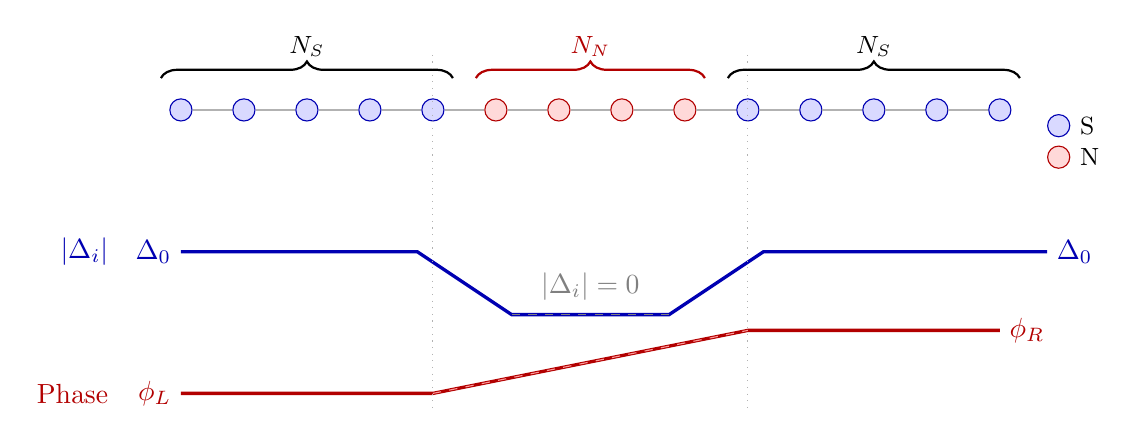
\begin{tikzpicture}[
  siteS/.style={circle,draw=blue!70!black,fill=blue!15,inner sep=2pt,minimum size=8pt},
  siteN/.style={circle,draw=red!70!black,fill=red!15,inner sep=2pt,minimum size=8pt},
  bond/.style={thick,color=gray!60},
  brace/.style={decorate,decoration={brace,amplitude=6pt},thick}
]

\def\NL{5}
\def\NN{4}
\def\NR{5}
\pgfmathtruncatemacro{\Ntot}{\NL+\NN+\NR}
\def\sp{0.8cm}

\foreach \i in {1,...,\Ntot} {
  \pgfmathtruncatemacro{\itype}{ (\i <= \NL ? 1 : (\i <= \NL+\NN ? 2 : 3)) }
  \ifnum\itype=1
    \node[siteS] (s\i) at (\i*\sp,0) {};
  \else\ifnum\itype=2
    \node[siteN] (s\i) at (\i*\sp,0) {};
  \else
    \node[siteS] (s\i) at (\i*\sp,0) {};
  \fi\fi
}
\foreach \i in {1,...,\Ntot} {
  \pgfmathtruncatemacro{\j}{\i+1}
  \ifnum\i<\Ntot \draw[bond] (s\i) -- (s\j); \fi
}

\draw[brace] ($(s1.north west)+(-0.15,0.3)$) --
  node[above=4pt,font=\small] {$N_S$} ($(s\NL.north east)+(0.15,0.3)$);
\draw[brace,red!70!black] ($(s\the\numexpr\NL+1\relax.north west)+(-0.15,0.3)$) --
  node[above=4pt,font=\small] {$N_N$} ($(s\the\numexpr\NL+\NN\relax.north east)+(0.15,0.3)$);
\draw[brace] ($(s\the\numexpr\NL+\NN+1\relax.north west)+(-0.15,0.3)$) -- node[above=4pt,font=\small] {$N_S$} ($(s\Ntot.north east)+(0.15,0.3)$);

\node[siteS,label=right:{\small S},anchor=west] at ($(s\Ntot)+(0.6,-0.2)$) {};
\node[siteN,label=right:{\small N},anchor=west] at ($(s\Ntot)+(0.6,-0.6)$) {};

\def\xFirst{0.8}
\def\xL{4.0}
\def\xNL{4.8}
\def\xNR{7.2}
\def\xR{8.0}
\def\xLast{11.2}
\def\hoff{0.2}
\def\xExt{0.6}

\def\magHigh{-1.8}
\def\magLow{-2.6}
\def\phBot{-3.6}
\def\phTop{-2.8}

\draw[blue!70!black, very thick]
  (\xFirst, \magHigh) --                                 % début
  (\xL - \hoff, \magHigh) --                            % plat gauche
  (\xNL + \hoff, \magLow) --                            % descente
  (\xNR - \hoff, \magLow) --                            % plat zéro
  (\xR + \hoff, \magHigh) --                            % montée
  (\xLast + \xExt, \magHigh);                           % plat droit 

\draw[dashed,gray] (\xNL + \hoff, \magLow) -- (\xNR - \hoff, \magLow);

\node[blue!70!black,left] at (\xFirst, \magHigh) {$\Delta_0$};
\node[blue!70!black,right] at (\xLast + \xExt, \magHigh) {$\Delta_0$};
\node[gray] at ({(\xNL+\xNR)/2}, \magLow+0.8) [below=4pt] {$|\Delta_i|=0$};

\draw[red!70!black, very thick]
  (\xFirst, \phBot) --                                   % début gauche
  (\xL, \phBot) --                                       % plat gauche
  (\xR, \phTop) --                                       % rampe linéaire
  (\xLast, \phTop);                                      % plat droit
\draw[dashed,red!40] (\xL, \phBot) -- (\xR, \phTop);

\node[red!70!black,left] at (\xFirst, \phBot) {$\phi_L$};
\node[red!70!black,right] at (\xLast, \phTop) {$\phi_R$};


\node[blue!70!black,left] at (\xFirst - 0.8, \magHigh) {$|\Delta_i|$};
\node[red!70!black,left] at (\xFirst - 0.8, \phBot) {Phase};


\foreach \x in {\xL,\xNR+0.8} {
  \draw[dotted,thin,gray!60] (\x, \magHigh + 2.5) -- (\x, \phBot - 0.2);
}

\end{tikzpicture}
\caption{One-dimensional tight-binding model of an SNS junction.}
\label{fig:sns_model}
\end{figure}


The total length is \(N = 2N_S + N_N\).  The hopping between all neighboring sites is \(t\). We do not introduce additional interface barriers, so the only source of normal reflection is a possible Fermi-wavevector mismatch \(\mu_N \neq \mu_S\).

\subsection{Self-consistency and phase boundary conditions}

To obtain the order parameter profile we iterate the BdG equations as outlined in Appendix~\ref{app:numerical implementation}.  The key choice is how we treat the phase in order to deal with current conservation.

\begin{itemize}
  \item \textbf{Fixed phase in the leads (FPL).}  The complex order parameter in the left and right leads is pinned to \(\Delta_{L,R} = |\Delta_{L,R}|\,e^{\mathrm{i}\phi_{L,R}}\). It forces the entire phase drop to occur across the normal region. The drawback is that the leads carry zero supercurrent, which is inconsistent with current conservation.
  \item \textbf{Fixed phase at the boundaries (FPB).}  Only the order parameters on the few first sites and the last sites are held fixed at \(\phi_L\) and \(\phi_R\).  All other sites, including those in the leads, are free to relax both in magnitude and phase.  This allows a phase gradient to develop inside the superconductors, which restores current conservation.  The effective phase difference across the normal region is then smaller than the total bias \(\phi_R-\phi_L\) because part of the phase drop is taken up by the leads.
\end{itemize}

\subsection{Current operator}

The current flowing from site $j$ to site $i$ is given by Eq.~\eqref{eq:J_final}. We average over a few central bonds to reduce numerical noise.

\section{Phase profile: FPL and FPB}

Before analyzing the CPR in detail, we compare the two phase-boundary conditions to understand how the supercurrent distributes itself in the junction. The phase plotted is the one of $F_i=\langle\hat{c}_{i\downarrow}\hat{c}_{i\uparrow}\rangle$ as the phase of $\Delta_i=UF_i$ is not defined in the normal region where $U=0$.

\begin{figure}[H]
  \centering
  \begin{subfigure}[b]{0.48\textwidth}
    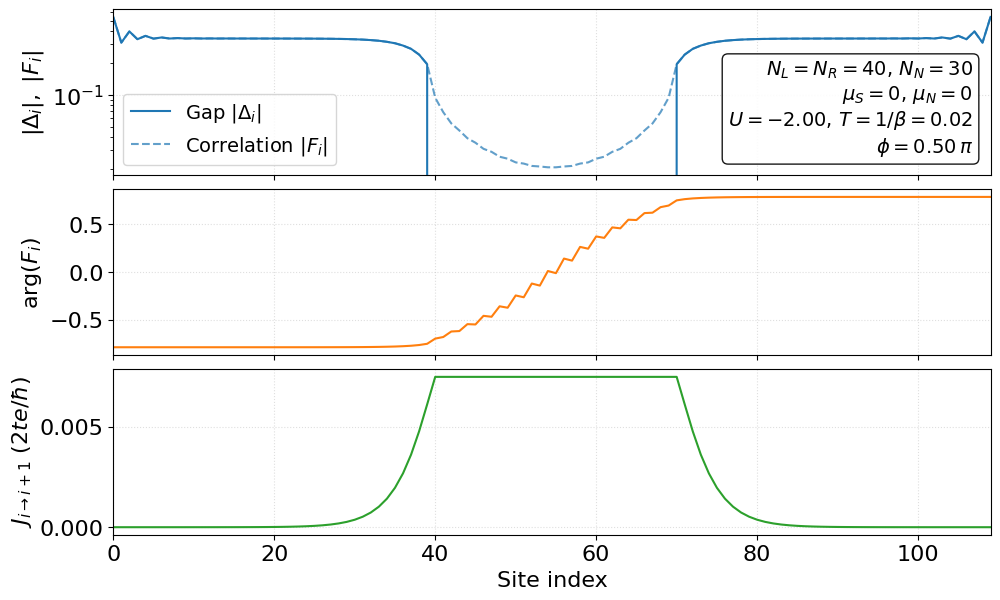
\includegraphics[width=\textwidth]{figures/ch5_phase_profile_fpl.png}
    \caption{Fixed Phase in the Leads (FPL)}
    \label{fig:FPL}
  \end{subfigure}
  \hfill
  \begin{subfigure}[b]{0.48\textwidth}
    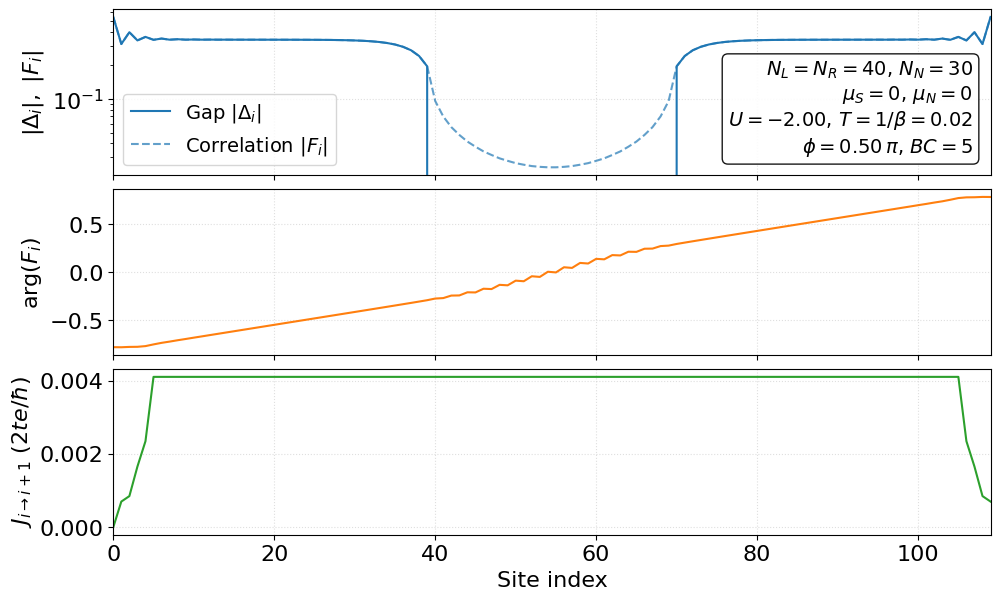
\includegraphics[width=\textwidth]{figures/ch5_phase_profile_fpb.png}
    \caption{Fixed Phase at the Boundaries (FPB)}
    \label{fig:FPB}
  \end{subfigure}
  \caption{Comparison of FPL and FPB schemes.}
  \label{fig:phase_comparison}
\end{figure}


The comparison of Fig.~\ref{fig:phase_comparison} confirms that the FPB scheme is physically more consistent: a supercurrent flows in the leads. However, it is accompanied by a phase gradient.



\section{Current-phase relation}


In this section we present the current-phase relation for various junction parameters.


\subsection{Fully transparent junction}

When the chemical potentials in the normal region and the superconductor are matched
($\mu_N=\mu_S$), the junction is free of Fermi-wavevector mismatch and is
therefore maximally transparent. The characteristic length scale that separates
short from long junctions is the ballistic superconducting coherence length
\begin{equation}
  \xi_0 = \frac{\hbar v_F}{\Delta_0}
        = \frac{2 t a \sin(k_F a)}{\Delta_0},
  \label{eq:xi0}
\end{equation}
where $k_F a = \arccos(-\mu_S/2t)$ and $\Delta_0$ is the zero-temperature gap. With our parameters ($t=1$, $a=1$, $\mu_S=0$, $\Delta_0\approx 0.1$) we find $\xi_0 \approx 20$ sites.  A junction is short when its length $L = N_N a \ll \xi_0$, and long when $L \gg \xi_0$. Since the tight-binding BdG solver includes all excitations across the full band, the simple estimate based on the Fermi velocity is only approximate. In practice the effective coherence length is smaller, typically $\xi_0\approx 10$ sites for our parameters.

In the long-junction regime the fixed-phase-in-leads (FPL) and the
fixed-phase-at-boundaries (FPB) methods produce essentially identical
current-phase relations, as demonstrated in Fig.~\ref{fig:FPB vs FPL long junction}. The phase drop needed to sustain the supercurrent occurs mostly across the normal region. The weak phase gradient that remains in the leads has a negligible effect on the phase difference seen by the junction. Since the FPB scheme guarantees current conservation we adopt it for all long-junction simulations where the set of parameters allows us to reach the critical current.

For short junctions the FPB approach meets a practical limitation. Imposing a large total phase bias $\phi_R-\phi_L$ forces a steep phase gradient inside the superconducting leads. Most of the applied bias is then consumed by the leads, so the phase difference that actually develops across the short normal region remains well below the critical value $\phi_{\max}$ required to reach the critical supercurrent. In this situation FPB cannot trace the full CPR. It only explores the low-current region of the CPR.

To overcome this restriction we use the FPL method for short junctions. By
freezing the phase in the leads we force the entire phase bias to drop across the normal region, thereby gaining access to the complete CPR up to and beyond $\phi_{\max}$.  Although this boundary condition violates current conservation, the error is small for short, highly transparent junctions.  Indeed, the FPL approach has been shown to reproduce the current-conserving result ~\cite{krekels_current_2025}.

A fully current-conserving method that employs a self-consistently adjusted phase gradient in the leads has recently been introduced by Krekels~\emph{et~al.}~\cite{krekels_current_2025}. For the present work the FPL scheme is sufficient to obtain the complete CPR of short junctions with reliable accuracy.


\begin{figure}[H]
  \centering
  \begin{subfigure}[b]{0.45\textwidth}
    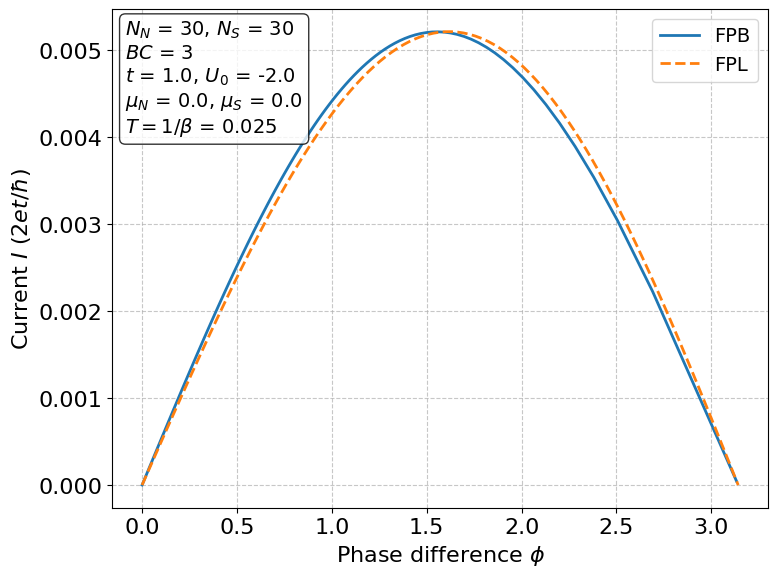
\includegraphics[width=\textwidth]{figures/ch5_cpr_fpb_vs_fpl_long.png}
    \caption{CPR for a long, fully transparent junction obtained with the FPB and FPL methods.}
    \label{fig:FPB vs FPL long junction}
  \end{subfigure}
  \hfill
  \begin{subfigure}[b]{0.45\textwidth}
    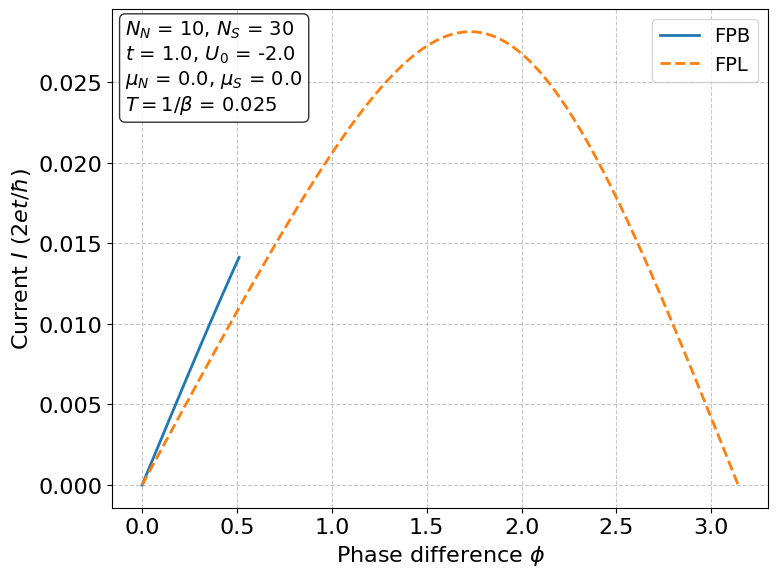
\includegraphics[width=\textwidth]{figures/ch5_cpr_fpb_vs_fpl_short.png}
    \caption{CPR for a short, fully transparent junction with the FPL method.}
    \label{fig:CPR_short_clean}
  \end{subfigure}
  \caption{Current-phase relation of a fully transparent SNS junction in the short and long regimes.}
  \label{fig:simple comp short long}
\end{figure}

In both the short-junction and long-junction limit, at high temperature, the CPR closely follows the form $I(\phi) \propto \sin(\phi)$, as shown in Fig.~\ref{fig:CPR_short_clean}. Both the critical current and the phase at which the maximum occurs (the critical phase) are affected by junction length, temperature, and normal-region transparency. The following sections analyze these deviations.



\subsection{Temperature dependence of the CPR}
\label{sec:Temperature dependence of the CPR}
As the temperature rises, the Fermi-Dirac distribution broadens, smearing the occupation of the Andreev bound states and modifying the shape of the CPR, causing the phase at which the critical current occurs to shift, and the critical current to decrease.

We explore these effects by simulating the fully transparent junction
($\mu_N=\mu_S$) for two representative lengths for a short junction and a long junction. The
temperature is varied from $T=0$ up to approximately $T_c$.

\begin{figure}[H]
  \centering
  \begin{subfigure}[b]{0.48\textwidth}
    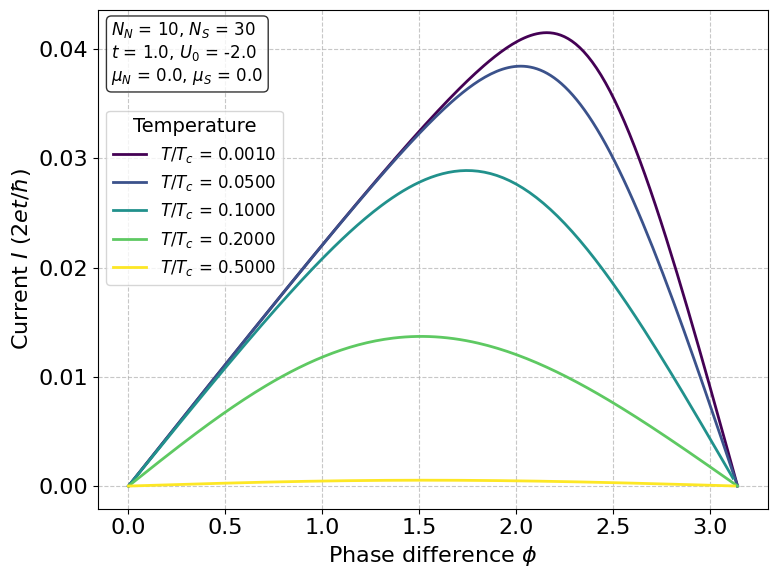
\includegraphics[width=\textwidth]{figures/ch5_cpr_temperature_short.png}
    \caption{CPR of the short, transparent junction at several temperatures (FPL).}
    \label{fig:CPR_temp_short}
  \end{subfigure}
  \hfill
    \begin{subfigure}[b]{0.48\textwidth}
    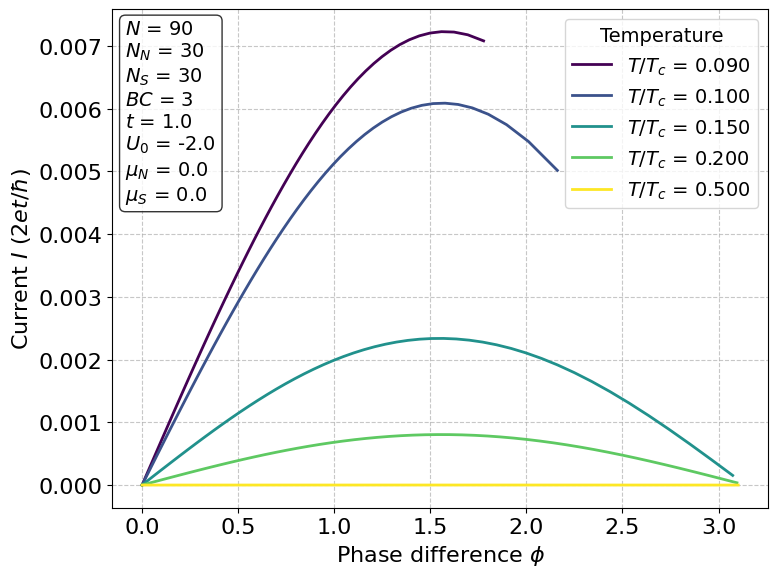
\includegraphics[width=\textwidth]{figures/ch5_cpr_temperature_long.png}
    \caption{CPR of the long, transparent junction at several temperatures (FPB).}
    \label{fig:CPR_temp_long}
  \end{subfigure}
  \caption{Temperature evolution of the current-phase relation for a fully transparent SNS junction.}
  \label{fig:CPR_temp_both}
\end{figure}

The CPR curves for the long junction~(Fig.~\ref{fig:CPR_temp_long}) are nearly $\sin(\phi)$ in the temperature range accessible to FPB. The amplitude decreases with $T$, while the shape remains essentially unchanged for this range of temperatures. In contrast, the
short-junction CPR~(Fig.~\ref{fig:CPR_temp_short}) shows a pronounced
non-sinusoidal behavior at low temperature, and gradually evolves toward a pure $\sin(\phi)$ shape as $T$ approaches $T_c$, with the amplitude also decreasing with $T$.

To quantify these observations we extract the critical current $I_{\max}(T)$ and the phase
$\phi_{\max}(T)$ at which the maximum occurs.  Both are plotted in Fig.~\ref{fig:crit_temp_both}.


\begin{figure}[H]
  \centering
  \begin{subfigure}[b]{0.48\textwidth}
    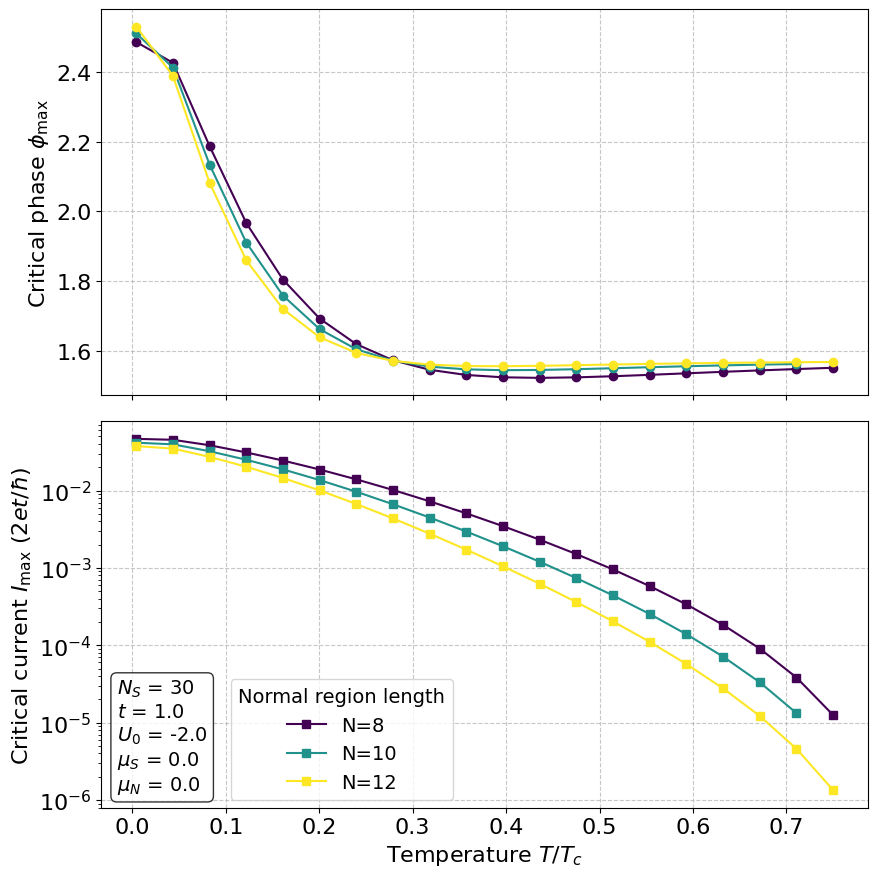
\includegraphics[width=\textwidth]{figures/ch5_critical_vs_temperature_short.png}
    \caption{Short junction (FPL).}
    \label{fig:crit_temp_short}
  \end{subfigure}
  \hfill
  \begin{subfigure}[b]{0.48\textwidth}
    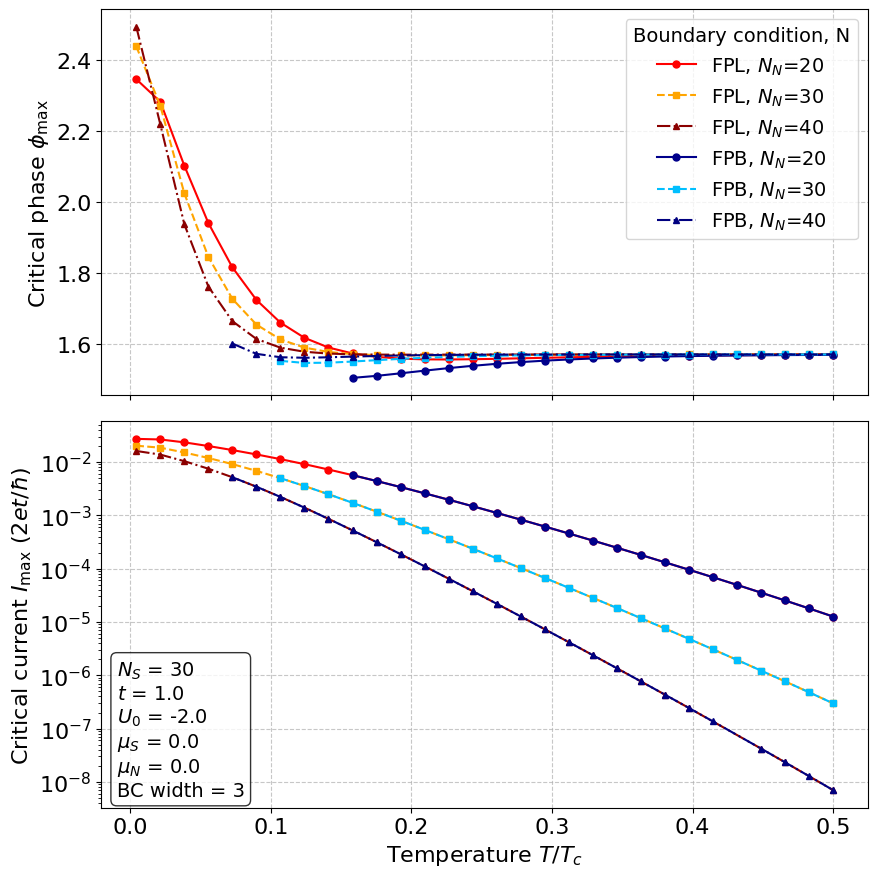
\includegraphics[width=\textwidth]{figures/ch5_critical_vs_temperature_long.png}
    \caption{Long junction (FPB and FPL).}
    \label{fig:crit_temp_long}
  \end{subfigure}
  \caption{Critical current $I_{\max}$ and critical phase $\phi_{\rm max}$ as functions of temperature for a fully transparent junction.}
  \label{fig:crit_temp_both}
\end{figure}

Both junctions exhibit a rapid decay of $I_{\max}$ with increasing temperature. The long junction’s critical current is, as expected, substantially smaller than that of the short junction because of the increased normal-region resistance. However they get close at low temperature. The behavior of the critical phase reveals a fundamental difference between
the two regimes:
\begin{itemize}
  \item \textbf{Short junction:} At $T=0$, $\phi_{\max}\approx\pi$, corresponding to a maximally forward-skewed CPR. As $T$ increases, $\phi_{\max}$ decreases and passes slightly below $\pi/2$, and then converges to $\pi/2$ as $T\rightarrow T_c$. This small dip can be attributed to the use of the FPL method, which does not conserve current.
  \item \textbf{Long junction:} Both boundary conditions produce a weak non-monotonic behavior. At $T=0$, $\phi_{\max}\approx\pi$, corresponding to a maximally forward-skewed CPR. As temperature increases, $\phi_{\max}$ first decreases, passes through a minimum, and then rises toward $\pi/2$ near $T_c$. The minimum is more pronounced in the current‑conserving FPB scheme. The FPL scheme also exhibits a minimum but of smaller amplitude.
\end{itemize}



This behavior remains qualitatively the same for a junction with Fermi level mismatch in superconductor and normal metal.


\subsection{Junctions with normal scattering: effect of Fermi-wavevector mismatch}

A junction is called mismatched when its normal region has a chemical potential $\mu_N$ different from that of the superconductors $\mu_S$. This mismatch in Fermi wave-vectors means that an electron approaching the NS interface from the normal side finds itself in a medium with a different electronic density. A fraction of the incident
probability is normally reflected back into the normal metal instead of being converted into a hole via Andreev reflection. The junction is no longer perfectly transparent. The transmission probability $\mathcal{T}$ for an electron crossing the normal region is reduced below unity.  As a result the current-phase relation is modified.

We study this effect by varying $\mu_N$ while keeping $\mu_S$ fixed at $0$. Figure~\ref{fig:crit_muN_both} summarizes the evolution of the critical current $I_{\max}$ and of the critical phase $\phi_{\rm max}$ for a short junction and a long junction.

\begin{figure}[H]
  \centering
  \begin{subfigure}[b]{0.32\textwidth}
    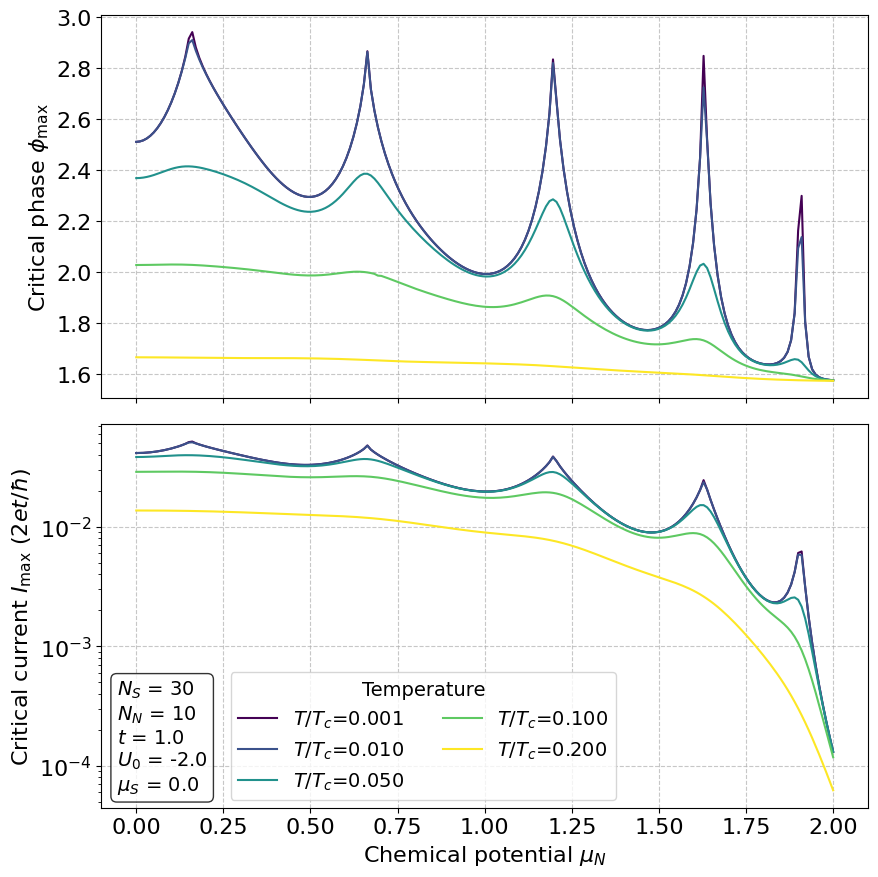
\includegraphics[width=\textwidth]{figures/ch5_critical_vs_muN_short.png}
    \caption{Short junction (FPL).}
    \label{fig:crit_muN_short}
  \end{subfigure}
  \hfill
  \begin{subfigure}[b]{0.32\textwidth}
    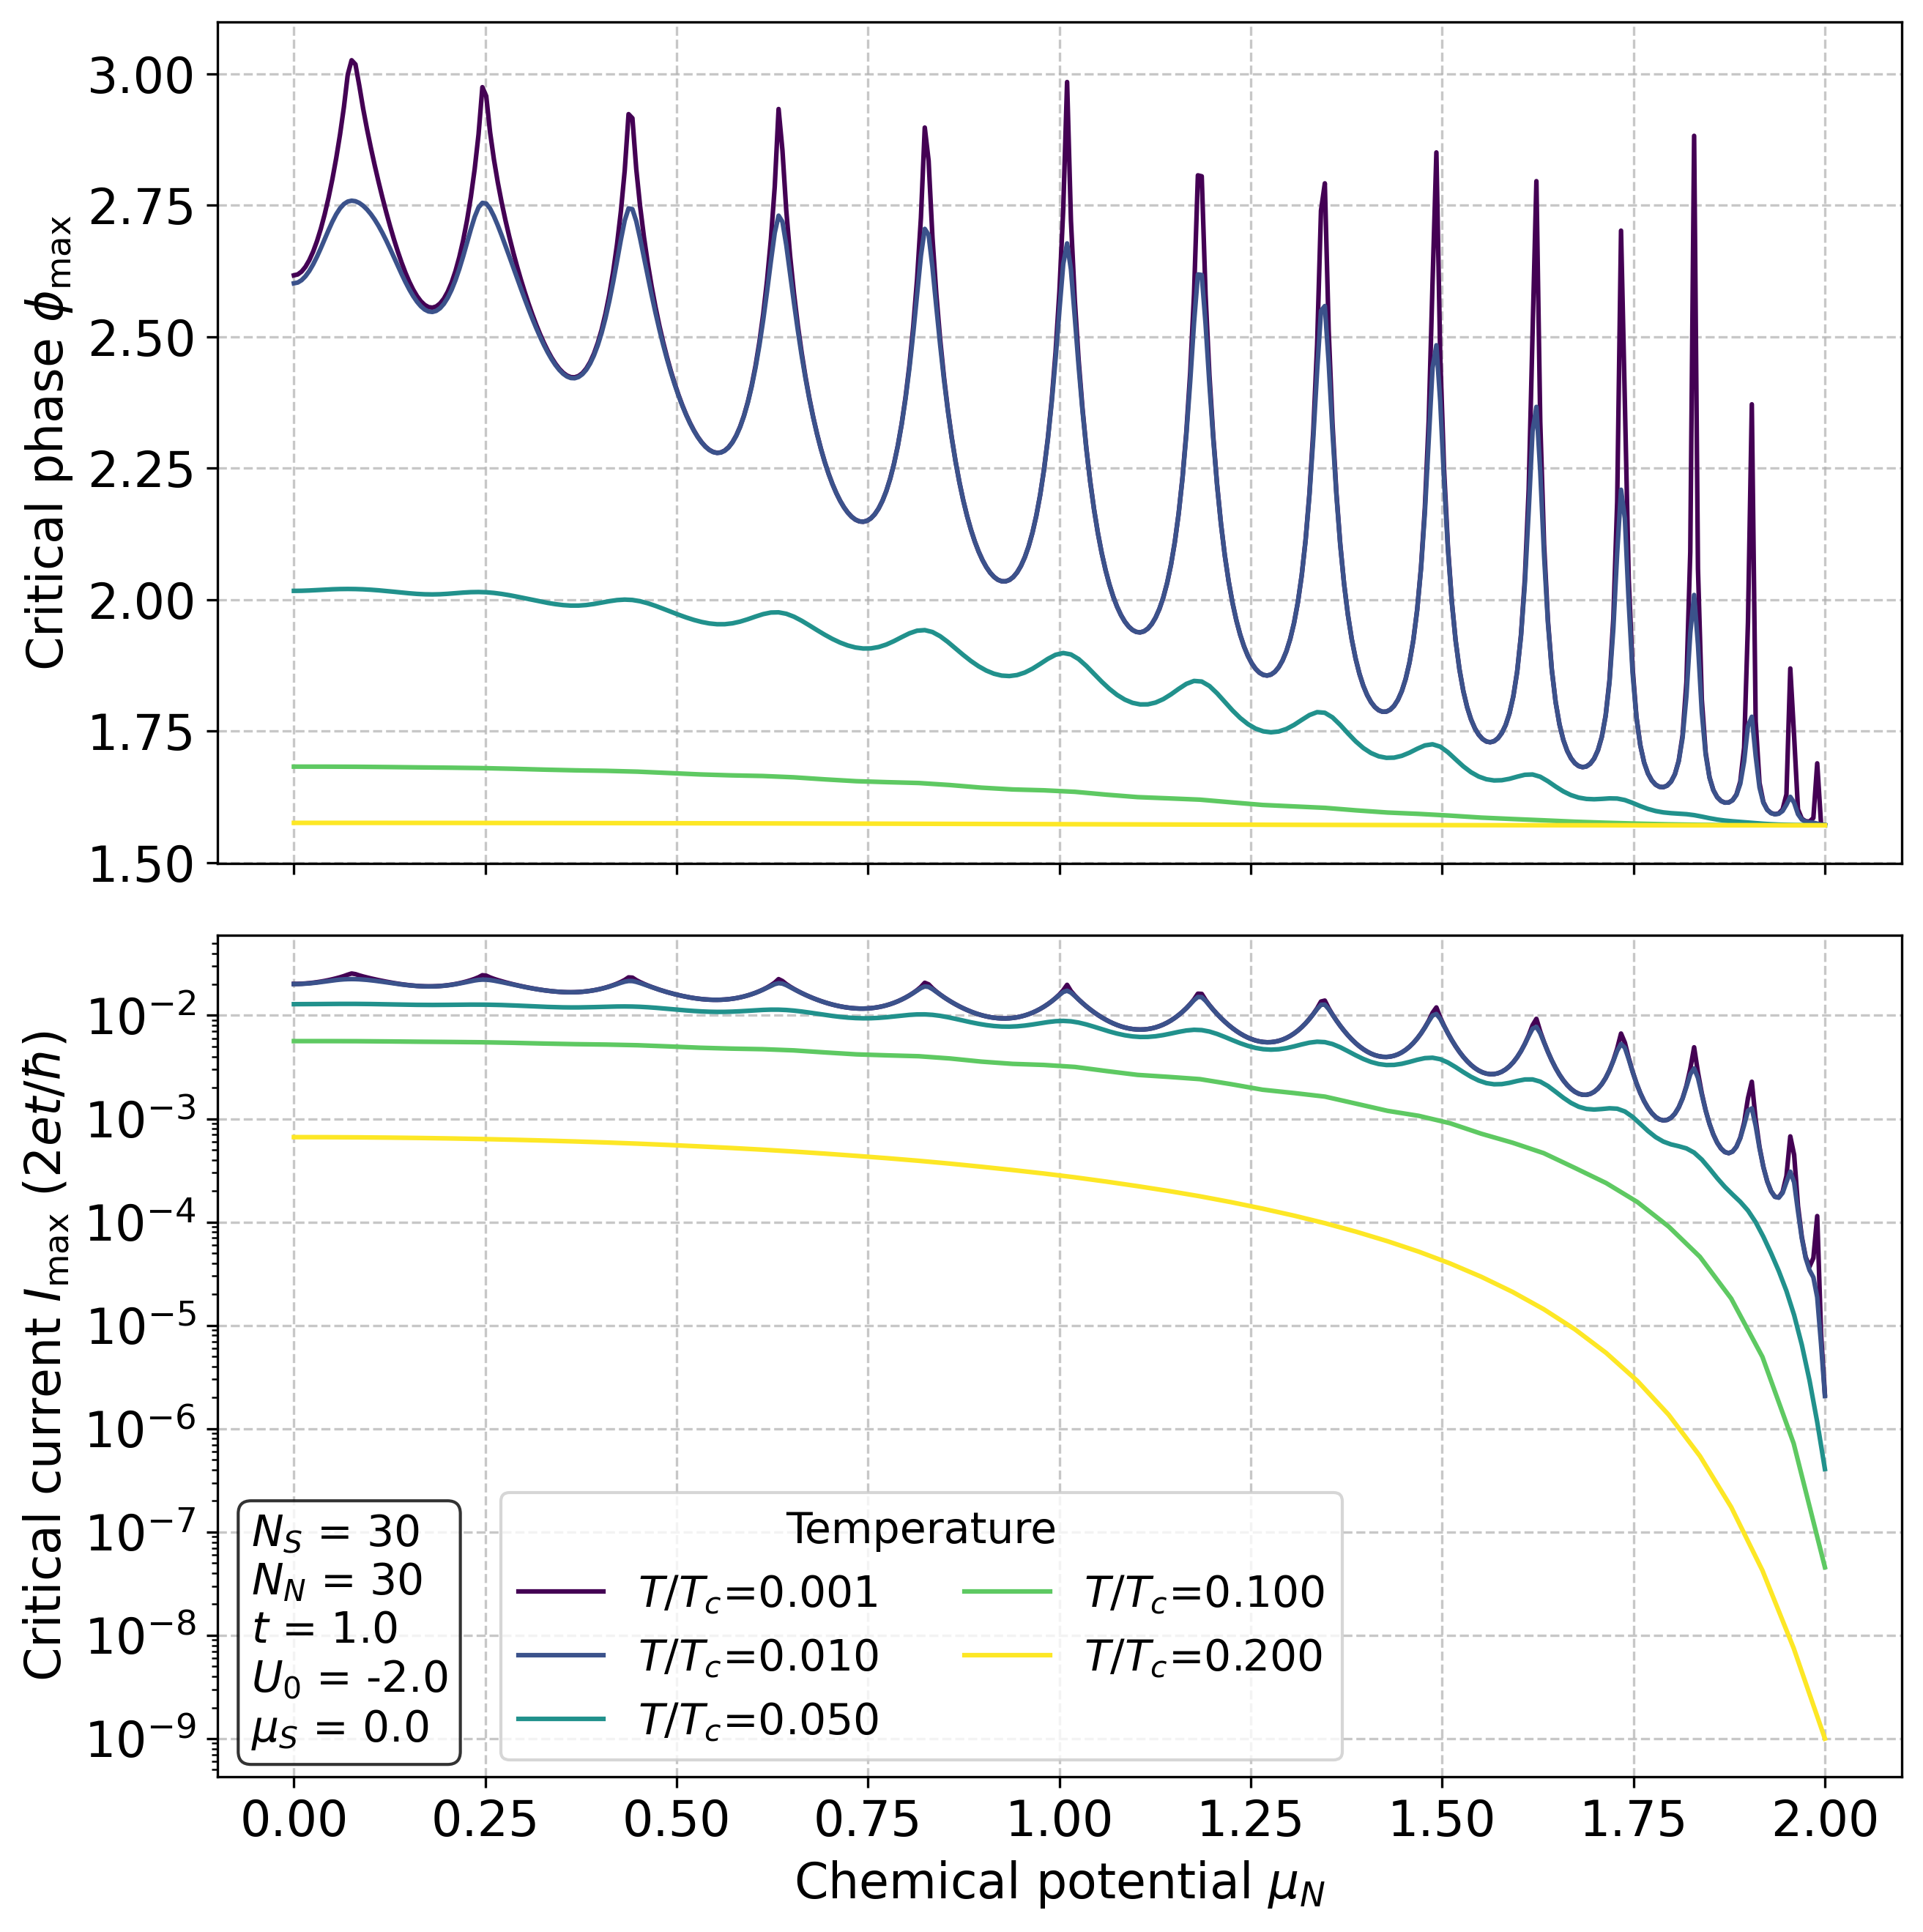
\includegraphics[width=\textwidth]{figures/ch5_critical_vs_muN_long_fpl.png}
    \caption{Long junction (FPL).}
    \label{fig:crit_muN_long_FPL}
  \end{subfigure}
  \hfill
  \begin{subfigure}[b]{0.32\textwidth}
    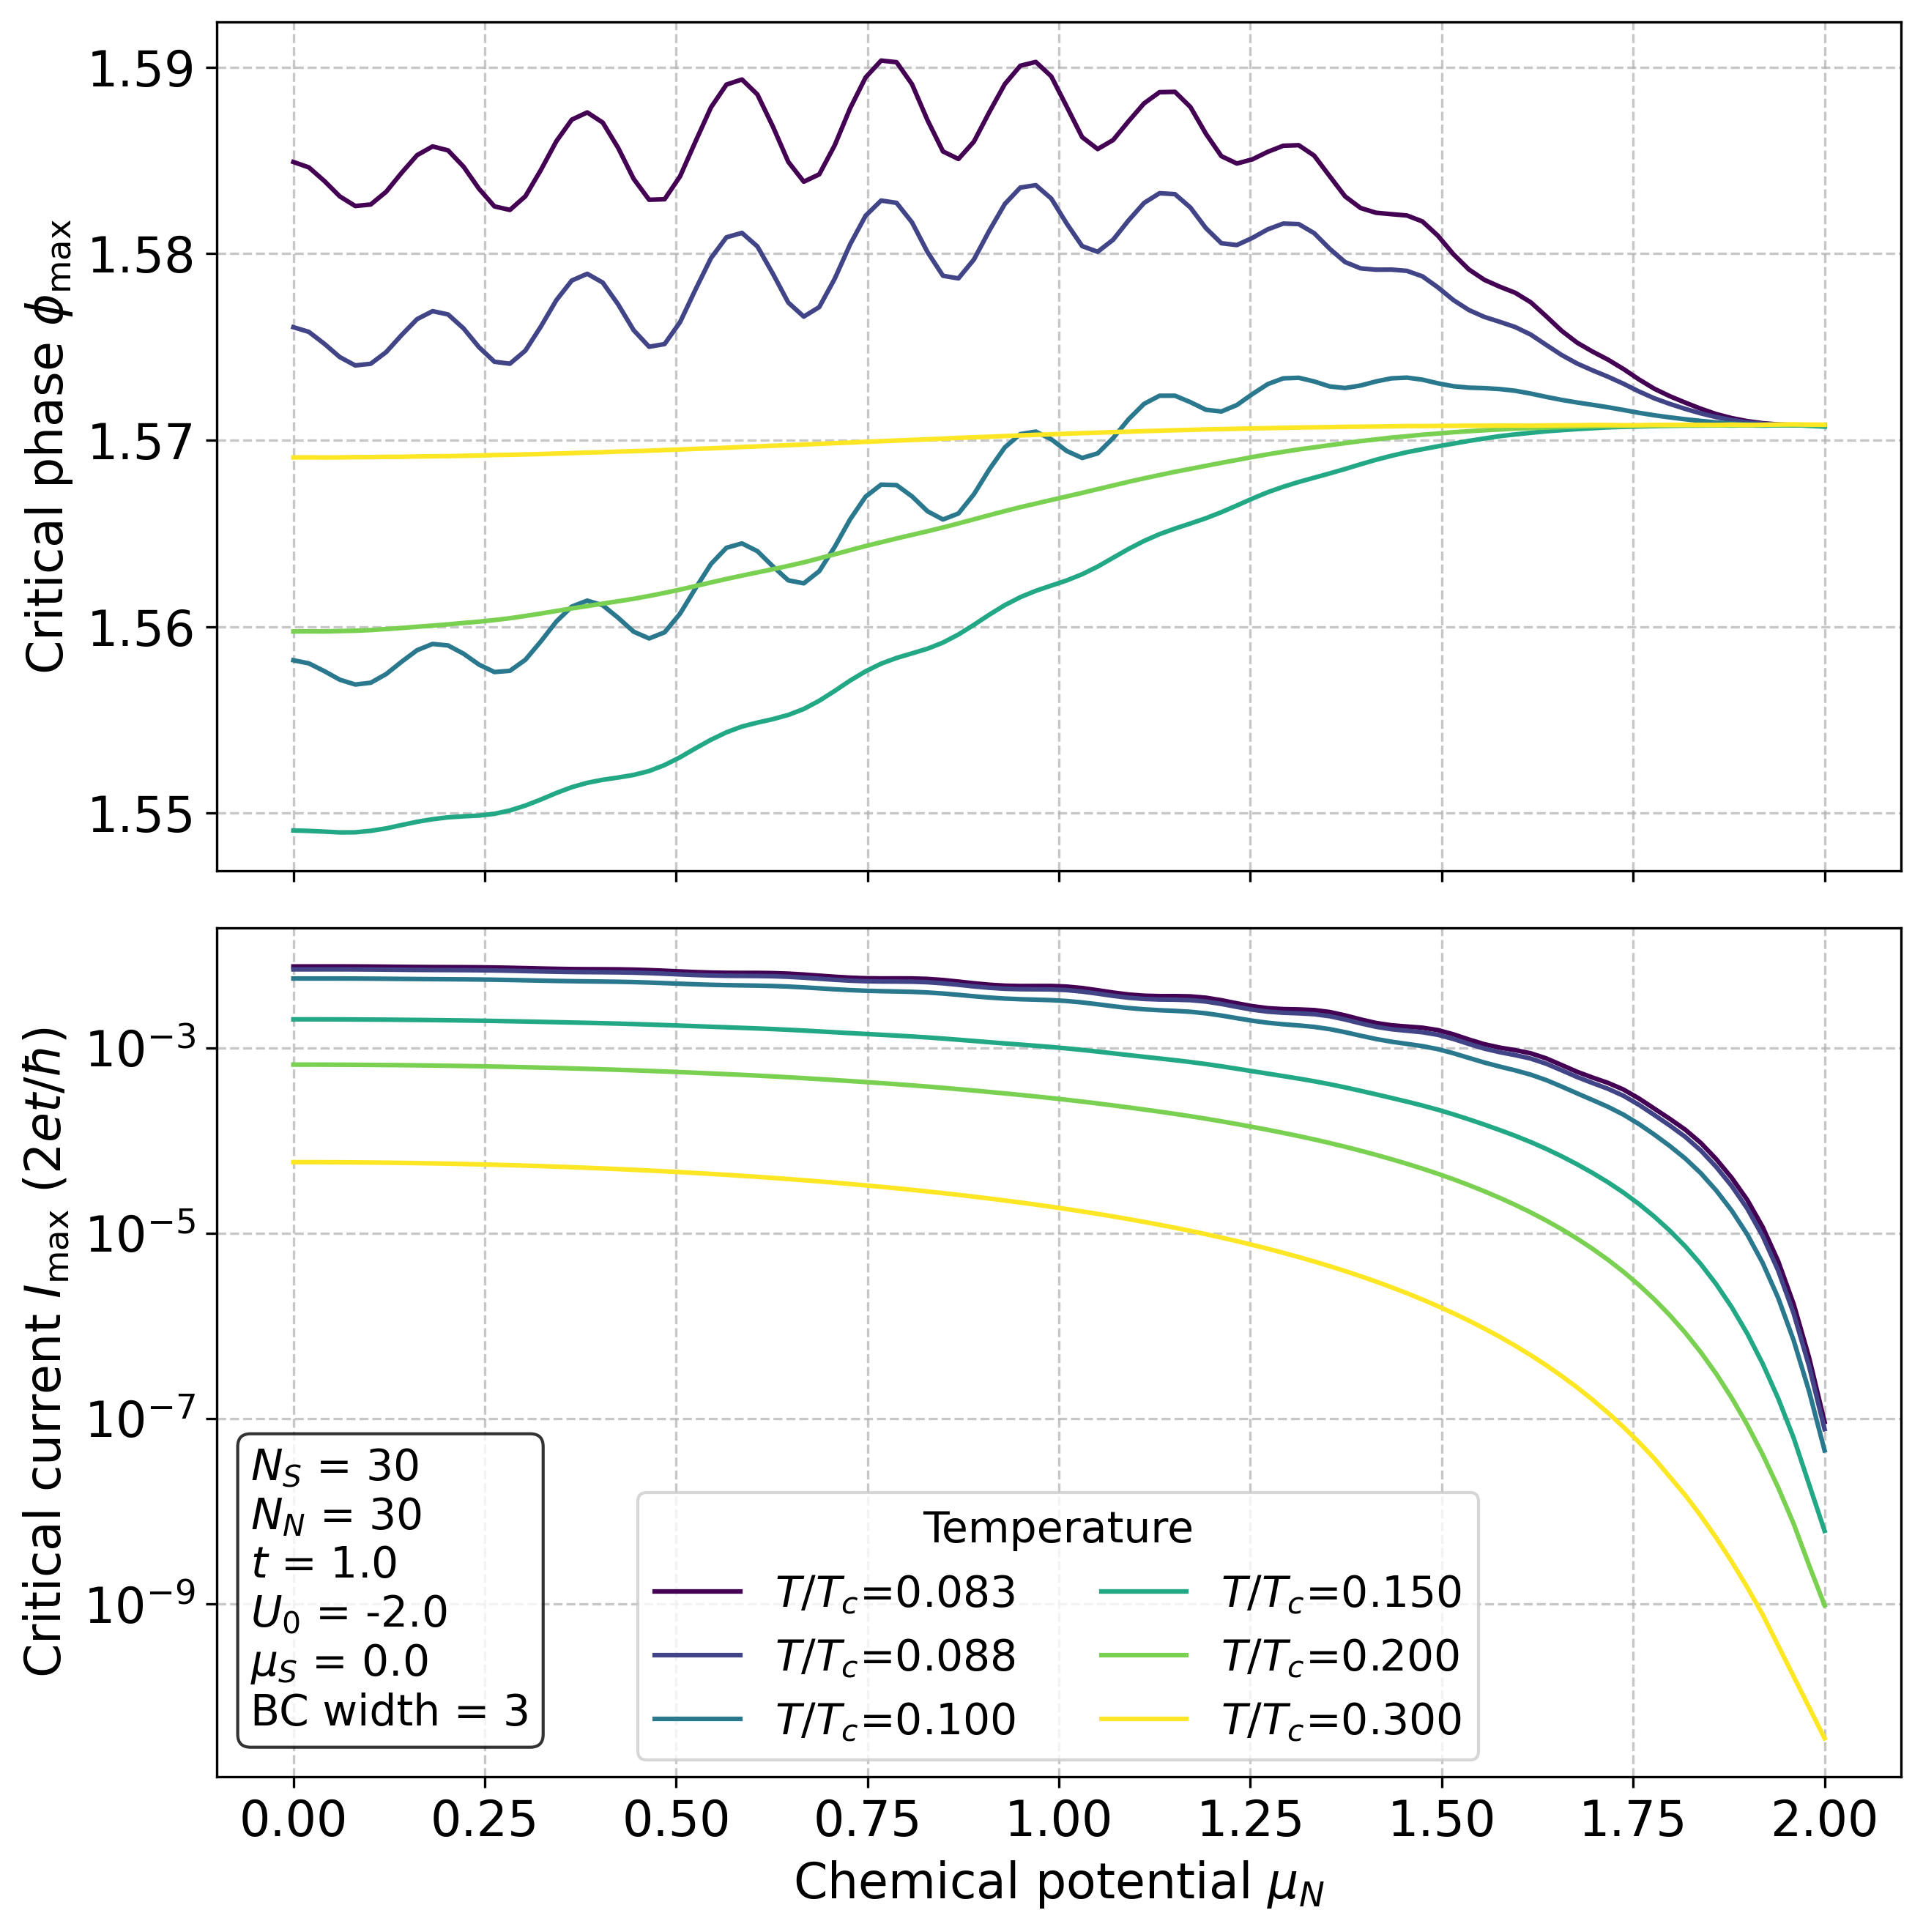
\includegraphics[width=\textwidth]{figures/ch5_critical_vs_muN_long_fpb.png}
    \caption{Long junction (FPB).}
    \label{fig:crit_muN_long}
  \end{subfigure}
  \caption{Critical current $I_{\max}$ and critical phase $\phi_{\rm max}$ as functions of the normal-region chemical potential $\mu_N$ for short and long mismatched junctions.}
  \label{fig:crit_muN_both}
\end{figure}
The oscillations are most clearly resolved using the FPL method (Figs.~\ref{fig:crit_muN_short} and~\ref{fig:crit_muN_long_FPL}) which forces the entire phase drop across the normal region at any temperature. At low temperature, we observe sharp, regularly spaced peaks in the critical phase. As temperature increases, the amplitude of these peaks decreases, but their positions remain unchanged. For finite mismatch, $\phi_{\max}$ evolves closer to $\pi/2$, reflecting the reduction in transparency. The critical current $I_{\max}$ generally decreases as $|\mu_N-\mu_S|$ grows, but small peaks correlated with the oscillations in $\phi_{\max}$ appear. For a given $\mu_N$, the current is higher for shorter junctions, as expected from the reduced normal‑region resistance. The number of oscillations scales linearly with the normal‑region length: a long junction with $N_N=30$ sites shows approximately $15$ distinct peaks, whereas a short junction with $N_N=10$ sites exhibits only about $5$ peaks over the same range. This is precisely the Fabry‑Pérot condition $k_{F,N}L=m\pi$ that will be discussed in detail in Section~\ref{sec:FabryPerot}.

For long junctions (Fig.~\ref{fig:crit_muN_long}), the FPB scheme is practical only at high temperatures. In this regime, the oscillations in $I_{\max}(\mu_N)$ and $\phi_{\max}(\mu_N)$ are still visible, but they are weakened and no longer appear as sharp peaks due to thermal smearing. Nevertheless, the wavelength of these oscillations remains the same as in the FPL simulations, suggesting an identical physical origin (Fabry‑Pérot interference in the normal region). Moreover, the FPB data clearly show the passage through the minimum in $\phi_{\max}(T)$ discussed in Section~\ref{sec:Temperature dependence of the CPR}, even though the accessible phase range is limited.



\begin{figure}[H]
  \centering
  \begin{subfigure}[b]{0.48\textwidth}
    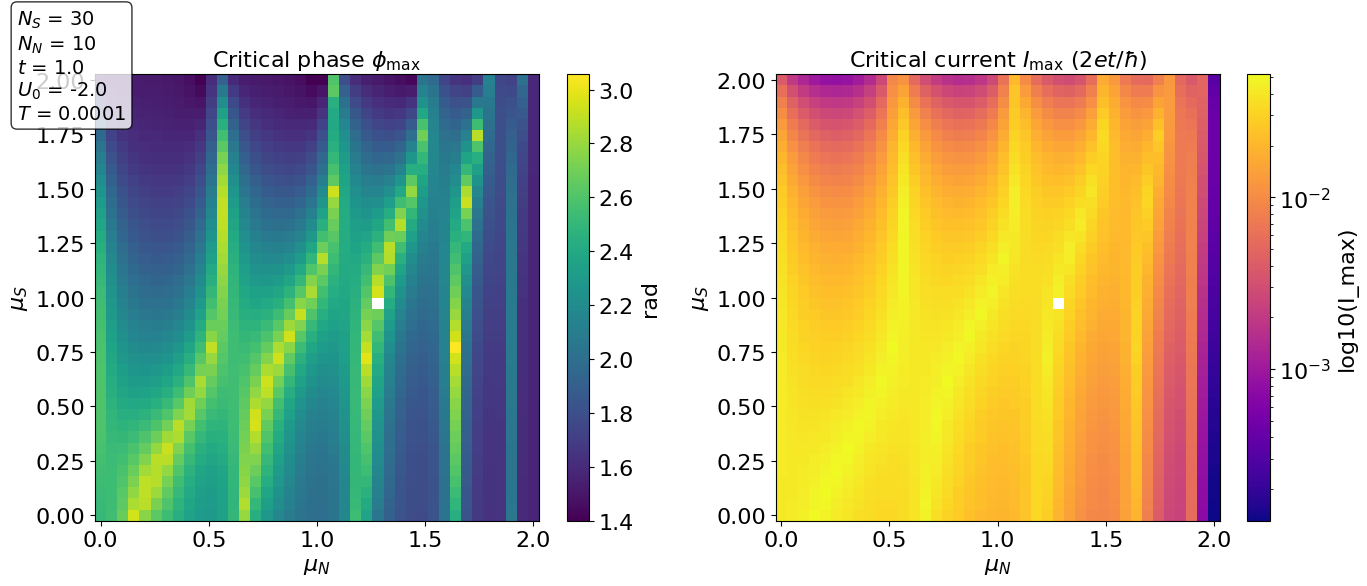
\includegraphics[width=\textwidth]{figures/ch5_critical_map_mu_low_temperature.png}
    \caption{Low temperature (FPL).}
    \label{fig:color grid muN muS low temp}
  \end{subfigure}
  \hfill
  \begin{subfigure}[b]{0.48\textwidth}
    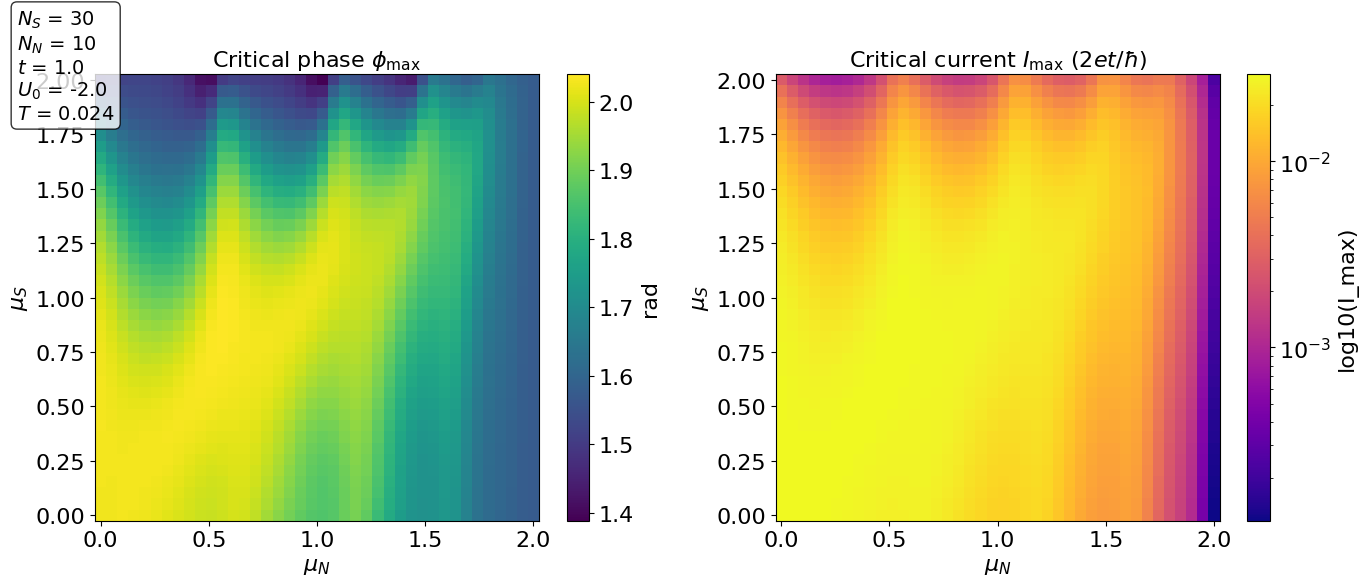
\includegraphics[width=\textwidth]{figures/ch5_critical_map_mu_high_temperature.png}
    \caption{High temperature (FPL).}
    \label{fig:color grid muN muS high temp}
  \end{subfigure}
  \caption{Critical current $I_{\max}$ and critical phase $\phi_{\rm max}$ as functions of $\mu_S$ and $\mu_N$ for a mismatched junction.}
    \label{fig:color grid muN muS}
\end{figure}

Critical current and critical phase as a function of $\mu_N$ and $\mu_S$ are shown in Fig.~\ref{fig:color grid muN muS} for two temperatures. At low temperature, both quantities exhibit sharp peaks as $\mu_N$ and $\mu_S$ vary. The positions of these peaks are essentially independent of temperature. At high temperature, the peaks are strongly suppressed in amplitude, the critical current is significantly lower, but the peak positions remain unchanged. Increasing the mismatch lowers the critical current. The detailed relationship between the oscillation patterns of $I_{\max}$ and $\phi_{\max}$ will be further explored in Section~\ref{sec:FabryPerot}.


\subsection{Length dependence of the critical current}

As the normal region grows longer, the supercurrent carried by each level is reduced. We investigate this effect by varying the normal-region length $N_N$ while keeping all other parameters fixed, and extract the critical current $I_\mathrm{max}$ for several temperatures $T/T_c$.

The results are presented in Fig.~\ref{fig:crit_curr_L}. At all temperatures the critical current decreases exponentially with $N_N$, with a rate that grows rapidly with temperature.


\begin{figure}[H]
    \centering
    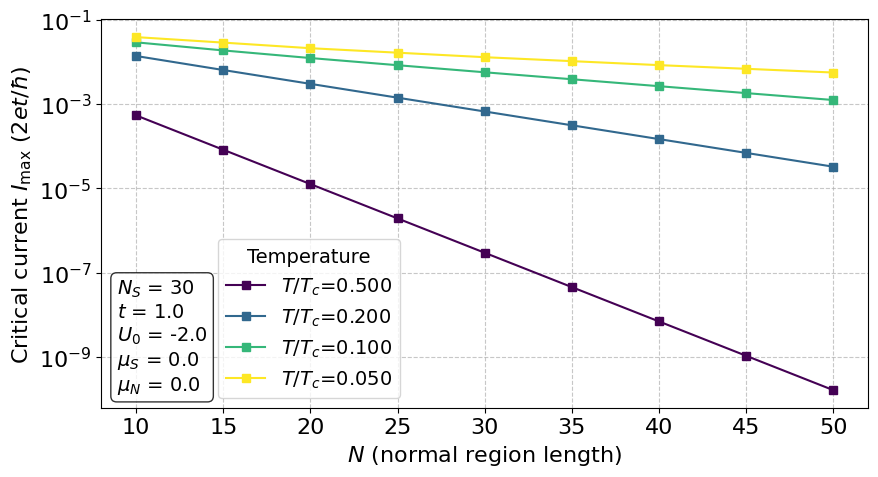
\includegraphics[width=0.5\linewidth]{figures/ch5_critical_vs_length.png}
    \caption{Critical current as a function of normal region length (FPL).}
    \label{fig:crit_curr_L}
\end{figure}


\chapter{Andreev bound states in the tight-binding model and the short-junction CPR}

The numerical simulations of Chapter~5 showed that a short SNS junction with matched chemical potentials exhibits a current-phase relation $I(\phi)\propto\sin(\phi)$ at high temperature. In this chapter we provide an analytical derivation of that result directly from the tight-binding Bogoliubov-de Gennes equations. We calculate the Andreev reflection amplitude at a normal-superconducting interface, construct the Andreev bound states of an SNS junction, and obtain the current-phase relation. Normal scattering caused by a Fermi-wave-vector mismatch is included via the scattering-matrix approach, leading to the single-channel Beenakker formula. The analytical predictions are compared with the self-consistent numerical results from Chapter~5.


\section{From phase difference to supercurrent}

We begin by establishing the relation between the phase of the order parameter and
the electrical current.  Consider the s-wave BdG Hamiltonian~\eqref{eq:H_MF_s-wave}
on a one-dimensional chain.  The pairing potential on site $i$ is
$\Delta_i = |\Delta_i| e^{\mathrm{i}\theta_i}$.  Let us perform a site-dependent gauge
transformation
\begin{equation}
  \hat{c}_{i\sigma} \;\longrightarrow\; \hat{c}_{i\sigma}\, e^{\mathrm{i}\theta_i/2}, \qquad
  \hat{c}_{i\sigma}^{\dagger} \;\longrightarrow\; \hat{c}_{i\sigma}^{\dagger}\, e^{-\mathrm{i}\theta_i/2}.
\end{equation}
In the new basis the order parameter becomes purely real, $\Delta_i \to |\Delta_i|$,
while the hopping amplitudes acquire a phase factor
\begin{equation}
  t_{ij} \;\longrightarrow\; t_{ij}\, \exp\!\bigl[\mathrm{i}(\theta_j - \theta_i)/2\bigr].
\end{equation}
The single-particle part of the Hamiltonian therefore takes the form
\begin{equation}
  H' = \sum_{\langle ij\rangle,\sigma}
       t_{ij}\, e^{\mathrm{i}(\theta_j-\theta_i)/2}\,\hat{c}_{i\sigma}^{\dagger}\hat{c}_{j\sigma},
  \label{eq:Peierls}
\end{equation}
where the phase of the order parameter has been converted into a phase factor on the
hopping.  This is precisely a Peierls substitution with a vector potential $\mathbf{A}$ such that
\begin{equation}
  \frac{e}{\hbar}\int_{\mathbf{r}_i}^{\mathbf{r}_j} \mathbf{A}\cdot d\mathbf{l}
  = \frac{\theta_j-\theta_i}{2}.
\end{equation}
The correspondence allows us to identify the phase gradient as the driving force for
the supercurrent.

The current operator is obtained from the functional derivative of the Hamiltonian
with respect to the vector potential.  In the continuum, the current density
$\hat{\mathbf{j}}(\mathbf{r})$ satisfies
\begin{equation}
  \delta\hat{H} = -\int d\mathbf{r}\;\hat{\mathbf{j}}(\mathbf{r})\cdot \delta\mathbf{A}(\mathbf{r}).
\end{equation}
On the other hand, a variation of the phase differences $\theta_j-\theta_i$ in the
discrete Hamiltonian can be expressed through $\delta\mathbf{A}$ as
\begin{equation}
  \delta\hat{H}
  = \sum_{\langle ij\rangle} \frac{\partial\hat{H}}{\partial(\theta_j-\theta_i)}\,
    \delta(\theta_j-\theta_i)
  = \frac{2e}{\hbar} \sum_{\langle ij\rangle} \frac{\partial\hat{H}}{\partial(\theta_j-\theta_i)}
    \int_{\mathbf{r}_i}^{\mathbf{r}_j} \delta\mathbf{A}\cdot d\mathbf{l}.
\end{equation}
Comparing the two expressions and identifying the coefficients of $\delta\mathbf{A}$,
we obtain the current operator as
\begin{equation}
  \hat{\mathbf{j}}(\mathbf{r})
  = -\frac{2e}{\hbar} \sum_{\langle ij\rangle} \frac{\partial\hat{H}}{\partial(\theta_j-\theta_i)}
  = -\frac{2e}{\hbar}\,\frac{\partial\hat{H}}{\partial\phi},
\end{equation}
where $\phi \equiv \theta_R - \theta_L$ is the total phase difference across the junction.

We are now in a position to connect the supercurrent to the quasiparticle spectrum. The BdG Hamiltonian may be diagonalized, giving $\hat{H}_{\rm MF} = E_g + \sum_{n,\sigma} E_n \hat{\gamma}_{n\sigma}^{\dagger} \hat{\gamma}_{n\sigma}$. Differentiating with respect to $\phi$ and taking the thermal expectation value, we find
\begin{equation}
  \boxed{
  I(\phi) = \frac{2e}{\hbar} \sum_{n} \frac{\partial E_n}{\partial\phi}\, f(E_n) ,
  }
  \label{eq:I_from_spectrum}
\end{equation}
where $f(E) = 1/(e^{\beta E}+1)$ is the Fermi-Dirac distribution. This formula reduces the calculation of the Josephson current to determining the phase dependence of the quasiparticle eigenenergies.

\section{General method for comparison with short-junction theories}
\label{sec:square_well_method}
While the self-consistent BdG loop of Chapter~5 provides the most accurate description of an SNS junction, it can obscure the comparison with the analytical theories developed in this chapter.  The reason is twofold.
\begin{enumerate}
  \item Self-consistency adjusts the magnitude and phase of $\Delta_i$ everywhere, so the final order-parameter profile differs from the idealized step function used in the analytical derivations.
  \item For large supercurrents (when phase difference is large ($\phi\approx\pi$) and normal-region length is small), the self-consistent gap is strongly suppressed and the iterative scheme may converge slowly or even jump between metastable branches, making it difficult to obtain clean numerical data.
\end{enumerate}
To overcome these difficulties and to test the analytical predictions under the same assumptions they were derived with, we temporarily abandon self-consistency and instead diagonalize the BdG matrix $\mathcal{H}$ once, with a frozen pair potential of the form
\begin{equation}
  \Delta_i = \begin{cases}
    \Delta_0\,e^{\mathrm{i}\phi_L}, & x< -L/2,\\[4pt]
    0,                     & -L/2\le x\le L/2 ,\\[4pt]
    \Delta_0\,e^{\mathrm{i}\phi_R}, & x > L/2.
  \end{cases}
  \label{eq:Delta_square}
\end{equation}

Here $\Delta_0$ is a constant gap amplitude and $\phi$ the imposed phase difference.  The hopping, chemical potentials, and all other parameters are the same as in the self-consistent simulations.  The current is then extracted from the eigenstates of this single-shot Hamiltonian using Eq.~\eqref{eq:J_final}, without any updates.

This approach offers exact control over the magnitude and phase of the pair potential, matching the step-function profile used in the analytical calculations, and keeps current conservation in the normal region.

The price is that we neglect the proximity-effect reduction of the gap near the interfaces and the phase re-arrangement inside the leads.  For short junctions ($L\ll\xi_0$) these effects are weak and the fixed-gap CPR reproduces the shape of self-consistent one with excellent accuracy, as shown in Fig.~\ref{fig:square_well}.
However, the amplitude differs due to nonuniform gap profile next to the interface.

\begin{figure}[H]
    \centering
    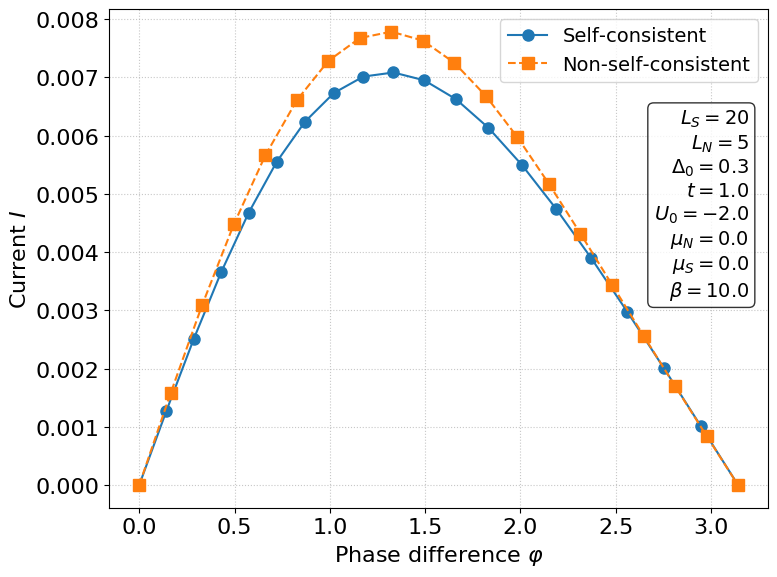
\includegraphics[width=0.6\textwidth]{figures/ch6_square_well_comparison.png}
    \caption{Comparison of the current-phase relation obtained from a single diagonalization with the fixed step-function gap~\eqref{eq:Delta_square} (points) and the corresponding self-consistent solution.}
    \label{fig:square_well}
\end{figure}


In the following sections we employ this fixed-gap scheme whenever we directly compare numerical and analytical results.

\section{General solutions of the tight-binding BdG equations}

To obtain the analytical spectrum of an SNS junction we idealize the pair potential by the step-function profile~\eqref{eq:Delta_square} where $x = i a$ and $L = N_N a$. The chemical potential in the normal metal is $\mu_N$, while the superconductors are assumed to be half-filled, i.e.\ $\mu_S = 0$, which places the Fermi wave-vector at $k_F a = \pi/2$.


\subsection{Normal region ($\Delta = 0$)}
\label{sec:gen_sol_normal}
In a normal region the BdG equations~\eqref{eq:BdG_swave} decouple into two identical tight-binding problems for electrons and holes:
\begin{equation}
  E_n u_{n,i} = -\mu_N u_{n,i} - t\sum_{\langle ji\rangle} u_{n,j}, \qquad
  E_n v_{n,i} = \mu_N v_{n,i} + t\sum_{\langle ji\rangle} v_{n,j}.
  \label{eq:N_eq}
\end{equation}
We look for plane-wave solutions $u_{n,i} = e^{\mathrm{i} k a i}$, $v_{n,i} = e^{\mathrm{i} k a i}$.
Inserting the ansatz into \eqref{eq:N_eq} yields the dispersions
\begin{equation}
  E_n = -\mu_N - 2t\cos(k_e a), \qquad
  E_n = \mu_N + 2t\cos(k_h a).
  \label{eq:disp_N}
\end{equation}
Hence the general wavefunction in the normal region is a superposition of four independent plane waves:
\begin{equation}
  \Psi_{n,i} = c_e^+\begin{pmatrix} 1 \\ 0 \end{pmatrix} e^{\mathrm{i} k_e^+ a i}
              + c_e^-\begin{pmatrix} 1 \\ 0 \end{pmatrix} e^{\mathrm{i} k_e^- a i}
              + c_h^+\begin{pmatrix} 0 \\ 1 \end{pmatrix} e^{\mathrm{i} k_h^+ a i}
              + c_h^-\begin{pmatrix} 0 \\ 1 \end{pmatrix} e^{\mathrm{i} k_h^- a i},
  \label{eq:Psi_N_general}
\end{equation}
where the four wave-vectors satisfy
\begin{equation}
  \cos(k_e^\pm a) = -\frac{\mu_N + E_n}{2t}, \qquad
  \cos(k_h^\pm a) = -\frac{\mu_N - E_n}{2t}.
  \label{eq:cos_N}
\end{equation}
The sub-e$^\pm$ and h$^\pm$ labels refer to right- and left-moving electron and hole states, respectively.  At the Fermi level ($E_n=0$) the Fermi wave-vector $k_F$ is defined by $\mu_N = -2t\cos(k_F a)$.  For excitation energies small compared to the Fermi energy, we may linearize the dispersion near $k_F$.  Writing
\[
  k_e^\pm = \pm (k_F + \delta k), \qquad
  k_h^\pm = \pm (k_F - \delta k),
\]
and expanding $\cos(k a)$ to first order gives
\[
  \delta k = \frac{E_n}{2 t a \sin(k_F a)} \equiv \frac{E_n}{\hbar v_F},
  \qquad v_F = \frac{2 t a}{\hbar} \sin(k_F a),
\]
where $v_F$ is the Fermi velocity of the tight-binding chain.  The four solutions can thus be written as:
\begin{equation}
  \boxed{
  \Psi_{n}(x) = c_e^+ \begin{pmatrix} 1 \\ 0 \end{pmatrix} e^{\mathrm{i}(k_F + \delta k)x}
              + c_e^- \begin{pmatrix} 1 \\ 0 \end{pmatrix} e^{-\mathrm{i}(k_F + \delta k)x}
              + c_h^+ \begin{pmatrix} 0 \\ 1 \end{pmatrix} e^{\mathrm{i}(k_F - \delta k)x}
              + c_h^- \begin{pmatrix} 0 \\ 1 \end{pmatrix} e^{-\mathrm{i}(k_F - \delta k)x},
  }
  \label{eq:Psi_N_linear}
\end{equation}
with $x = i a$ and $\delta k = E_n/(\hbar v_F)$.

\subsection{Superconducting region ($\Delta \neq 0$) with $\mu_S = 0$}
\label{sec:gen_sol_superconducting}
For the superconductors we take $\mu_S = 0$, which is the half-filled band condition.  The BdG equations are
\begin{equation}
  \begin{pmatrix}
    -t\sum_{\langle ji\rangle} & \Delta_i \\
    \Delta_i^* & t\sum_{\langle ji\rangle}
  \end{pmatrix}
  \begin{pmatrix} u_{n,i} \\ v_{n,i} \end{pmatrix}
  = E_n \begin{pmatrix} u_{n,i} \\ v_{n,i} \end{pmatrix},
  \label{eq:S_eq}
\end{equation}
with $\Delta_i \equiv \Delta = \Delta_0 e^{\mathrm{i}\phi}$ inside a given superconductor.  We solve these equations with a Bloch-like ansatz, distinguishing two energy ranges.

\subsubsection{Propagating solutions: $|E_n| > |\Delta|$}

For energies above the gap we look for running waves.  Substitute
$\Psi_n(i) = \begin{pmatrix} u \\ v \end{pmatrix} e^{\pm \mathrm{i} k a i}$ into \eqref{eq:S_eq}:
\begin{align}
  E_n u &= -2t\cos(k a) u + \Delta v, \label{eq:U_eq}\\
  E_n v &= +2t\cos(k a) v + \Delta^* u . \label{eq:V_eq}
\end{align}
Multiplying the two equations gives
\begin{equation}
  \bigl[E_n + 2t\cos(k a)\bigr]\bigl[E_n - 2t\cos(k a)\bigr] = |\Delta|^2,
\end{equation}
which yields the BCS dispersion
\begin{equation}
  \cos^2(k a) = \frac{E_n^2 - |\Delta|^2}{4 t^2}.
  \label{eq:cos2_S}
\end{equation}
For $\mu_S=0$ the Fermi points are at $k_F a = \pi/2$, where $\cos(k_F a)=0$. Linearizing the dispersion near $k_F$ we set $k = k_F \pm \delta k$, with $\delta k \ll \pi/a$.  Using $\cos(k_F a \pm \delta k a) \approx \mp \delta k a$ one obtains
\begin{equation}
  \delta k = \frac{\sqrt{E_n^2 - |\Delta|^2}}{2 t a}
           = \frac{\sqrt{E_n^2 - |\Delta|^2}}{\hbar v_F}, \qquad v_F = \frac{2ta}{\hbar}.
  \label{eq:delta_k_S}
\end{equation}
The corresponding eigenvectors are obtained by solving, e.g., \eqref{eq:U_eq} for the ratio $V/U$:
\begin{equation}
  \frac{v}{u} = \frac{E_n + 2t\cos(k a)}{\Delta}
               \approx \frac{E_n \mp \sqrt{E_n^2 - |\Delta|^2}}{\Delta},
\end{equation}
where the $\mp$ sign refers to $k \approx k_F \pm \delta k$.  Normalizing the spinors to unity leads to the following general solution for $|E_n|> |\Delta|$:
\begin{equation}
  \boxed{
  \begin{aligned}
  \Psi_S(x) = &
    \frac{c_e^+\, e^{\mathrm{i}(k_F+\delta k)x} + c_e^-\, e^{-\mathrm{i}(k_F+\delta k)x}}
         {\sqrt{2E_n\bigl(E_n-\sqrt{E_n^2-|\Delta|^2}\bigr)}}
    \begin{pmatrix} \Delta \\[2pt] E_n - \sqrt{E_n^2-|\Delta|^2} \end{pmatrix} \\[4pt]
  + & \frac{c_h^+\, e^{-\mathrm{i}(k_F-\delta k)x} + c_h^-\, e^{\mathrm{i}(k_F-\delta k)x}}
         {\sqrt{2E_n\bigl(E_n+\sqrt{E_n^2-|\Delta|^2}\bigr)}}
    \begin{pmatrix} \Delta \\[2pt] E_n + \sqrt{E_n^2-|\Delta|^2} \end{pmatrix},
  \end{aligned}}
  \label{eq:Psi_S_above}
\end{equation}
where $c_e^\pm$ and $c_h^\pm$ are again amplitudes for electron- and hole-like quasiparticles.  The two spinors correspond to states with predominantly electron ($+$) and hole ($-$) character.

\subsubsection{Evanescent solutions: $|E_n| < |\Delta|$}

For subgap energies the wave-vectors acquire an imaginary part, signaling that quasiparticles cannot propagate in the superconductor.  We therefore look for solutions of the form $\Psi_n(i) = \begin{pmatrix} u \\ v \end{pmatrix} e^{(\pm \mathrm{i} k_F + \kappa) a i}$ with a real decay constant $\kappa$.  Using $\cos(k_F a)=0$, we have $e^{\pm i k_F a i} e^{\kappa a i}$ leading to
\[
  \cos(k a) \;\to\; \cos((\pm k_F - \mathrm{i}\kappa)a) = \pm \mathrm{i}\,\sinh(\kappa a).
\]
Inserting this into \eqref{eq:U_eq}--\eqref{eq:V_eq} gives
\begin{align}
  (E_n \pm 2 \mathrm{i} t \sinh(\kappa a)) u &= \Delta v, \\
  (E_n \mp 2 \mathrm{i} t \sinh(\kappa a)) v &= \Delta^* u,
\end{align}
and therefore
\begin{equation}
  \sinh^2(\kappa a) = \frac{|\Delta|^2 - E_n^2}{4 t^2}.
  \label{eq:sinh2}
\end{equation}
For $\kappa a \ll 1$ we may approximate $\sinh(\kappa a) \approx \kappa a$, yielding
\begin{equation}
  \kappa = \frac{\sqrt{|\Delta|^2 - E_n^2}}{\hbar v_F}, \qquad v_F = \frac{2ta}{\hbar}.
  \label{eq:kappa}
\end{equation}
The general subgap wavefunction in the superconducting region is therefore
\begin{equation}
  \boxed{
  \begin{aligned}
  \Psi_S(x) = &
    \frac{c_1\, e^{(\mathrm{i} k_F + \kappa)x} + c_2\, e^{-(\mathrm{i} k_F + \kappa)x}}
         {E_n - \mathrm{i}\Omega}
    \begin{pmatrix} E_n - \mathrm{i}\Omega \\ \Delta^* \end{pmatrix} \\[4pt]
  + & \frac{c_3\, e^{(-\mathrm{i} k_F + \kappa)x} + c_4\, e^{(\mathrm{i} k_F - \kappa)x}}
         {E_n + \mathrm{i}\Omega}
    \begin{pmatrix} E_n + \mathrm{i}\Omega \\ \Delta^* \end{pmatrix},
  \end{aligned}}
  \label{eq:Psi_S_below}
\end{equation}
with $\Omega = \sqrt{|\Delta|^2 - E_n^2}$ and $\kappa = \Omega/(\hbar v_F)$.

 

\subsection{Andreev reflection at a single NS interface}

We now apply the general solutions of Sections~\ref{sec:gen_sol_normal} and~\ref{sec:gen_sol_superconducting} to a normal metal ($x<0$) in perfect contact with a superconductor ($x>0$).  The pair potential is taken to be
\begin{equation}
  \Delta(x) = \begin{cases}
    0,                     & x < 0, \\
    |\Delta|\,e^{\mathrm{i}\phi},  & x > 0 .
  \end{cases}
\end{equation}
The Fermi wavevectors in the two halves are assumed equal, $k_{F,N}=k_{F,S}\equiv k_F$, which is the condition for a transparent interface without normal scattering.  The chemical potential in the superconductor is set to $\mu_S=0$ (half-filling, $k_F a=\pi/2$) as in the preceding section.


Let an electron-like quasiparticle be incident from the normal side with energy $|E|<|\Delta|$.  Since no propagating states exist in the superconductor at subgap energies, the incident electron must be reflected either as an electron (normal reflection) or as a hole (Andreev reflection).  The most general wavefunction compatible with the BdG equations is therefore
\begin{equation}
  \Psi(x) = \begin{cases}
    \displaystyle
    \begin{pmatrix} 1 \\ 0 \end{pmatrix} e^{\mathrm{i} k_e^+ x}
    + r_{ee} \begin{pmatrix} 1 \\ 0 \end{pmatrix} e^{\mathrm{i} k_e^- x}
    + r_{eh} \begin{pmatrix} 0 \\ 1 \end{pmatrix} e^{\mathrm{i} k_h^+ x},
    & x < 0, \\[14pt]
    \displaystyle
    t_1\begin{pmatrix} \Delta \\ E_n - i\Omega \end{pmatrix} e^{\mathrm{i} k_F x} e^{-\kappa x}
    + t_2\begin{pmatrix} \Delta \\ E_n + i\Omega \end{pmatrix} e^{-\mathrm{i} k_F x} e^{-\kappa x},
    & x > 0 .
  \end{cases}
  \label{eq:Psi_NS}
\end{equation}
Here the wavevectors in the normal region are, in the linearized approximation,
\[
  k_e^\pm = \pm(k_F+\delta k), \qquad
  k_h^\pm = \pm(k_F-\delta k), \qquad
  \delta k = \frac{E}{\hbar v_F},
\]
with $v_F = 2ta\sin(k_F a)/\hbar$.  

For a clean interface, both the wavefunction and its discrete derivative must be continuous at $x=0$
\begin{equation}
  \Psi(0^-) = \Psi(0^+), \qquad
  \Psi'(0^-) = \Psi'(0^+).
  \label{eq:matching}
\end{equation}

Since $E\ll E_F$, the energy-dependent shifts $\delta k$ and $\kappa$ are small compared to $k_F$.  It is therefore legitimate to set $\delta k = \kappa = 0$. Imposing~\eqref{eq:matching} on the ansatz~\eqref{eq:Psi_NS} gives a system of four linear equations for the four unknowns $r_{ee}, r_{eh}, t_1, t_2$


\begin{equation}
  \boxed{
  \begin{aligned}
    1 + r_{ee} &= \Delta\,(t_1 + t_2), \\
    r_{eh}      &= (E - \mathrm{i}\Omega)\,t_1 + (E + \mathrm{i}\Omega)\,t_2, \\
    1 - r_{ee}  &= \Delta\,(t_1 - t_2), \\
    r_{eh}      &= (E - \mathrm{i}\Omega)\,t_1 - (E + \mathrm{i}\Omega)\,t_2 .
  \end{aligned}}
  \label{eq:matching_eqs}
\end{equation}

We get

\begin{equation}
  \boxed{
  r_{eh} =\frac{E - \mathrm{i}\sqrt{|\Delta|^2 - E^2}}{|\Delta|\,e^{\mathrm{i}\phi}}= e^{-\mathrm{i}\arccos(E/|\Delta|)}\, e^{-\mathrm{i}\phi}, \qquad r_{ee} = 0.
  }
  \label{eq:Andreev_amplitude}
\end{equation}
The amplitude has unit modulus: the electron is always converted into a hole.

An analogous calculation for an incident hole gives
\begin{equation}
  \boxed{
  r_{he} = e^{-\mathrm{i}\arccos(E/|\Delta|)}\, e^{+\mathrm{i}\phi}, \qquad r_{hh} = 0.
  }
  \label{eq:Andreev_amplitude_hole}
\end{equation}



\section{Andreev bound states in a ballistic SNS junction}

We now form a full SNS junction by sandwiching a normal metal of length $L = N_N a$ between two semi-infinite superconductors with pair potentials $\Delta_L = \Delta_0 e^{\mathrm{i}\phi_L}$ and $\Delta_R = \Delta_0 e^{\mathrm{i}\phi_R}$.  The normal region is ballistic ($\mu_N = \mu_S$) and the interfaces are perfectly transparent.

\subsection{Wavefunction in the normal region and transfer matrix}

Inside the normal region ($-L/2 < x < L/2$) the order parameter vanishes.  The general subgap wavefunction is the superposition of four plane waves derived in Sec.~\ref{sec:gen_sol_normal},
\begin{equation}
  \Psi_N(x) = c_e^+ \begin{pmatrix} 1 \\ 0 \end{pmatrix} e^{\mathrm{i} k_e^+ x}
            + c_e^- \begin{pmatrix} 1 \\ 0 \end{pmatrix} e^{\mathrm{i} k_e^- x}
            + c_h^+ \begin{pmatrix} 0 \\ 1 \end{pmatrix} e^{\mathrm{i} k_h^+ x}
            + c_h^- \begin{pmatrix} 0 \\ 1 \end{pmatrix} e^{\mathrm{i} k_h^- x},
  \label{eq:Psi_N_ABS}
\end{equation}
with the wave-vectors
\begin{equation}
  k_e^\pm = \pm (k_F + \delta k), \qquad
  k_h^\pm = \pm (k_F - \delta k), \qquad
  \delta k = \frac{E}{\hbar v_F},
\end{equation}
and $v_F = 2 t a \sin(k_F a)/\hbar$.  It is convenient to organize the amplitudes into a four-component vector
\[
  \mathbf{c} = \bigl( c_e^+,\; c_h^-,\; c_e^-,\; c_h^+ \bigr)^{\mathsf T},
\]
where the first two entries are right-moving electron and left-moving hole, and the last two are left-moving electron and right-moving hole.  Propagating the wavefunction over a distance $d$ simply advances the phases of each component,
\begin{equation}
  \mathbf{c}(x+d) = M(d)\,\mathbf{c}(x), \qquad
  M(d) = \begin{pmatrix}
    \mathcal{P}(d) & 0 \\
    0 & \mathcal{P}(-d)
  \end{pmatrix},
  \label{eq:M_transfer}
\end{equation}
where

\begin{equation}
   \mathcal{P}(d) = \begin{pmatrix}
     e^{\mathrm{i} k_F d}\;e^{\mathrm{i} \delta k \, d} & 0 \\
    0 &  e^{-\mathrm{i} k_F d}\;e^{\mathrm{i} \delta k \, d}
  \end{pmatrix}.
  \label{eq:M_blocks}
\end{equation}

\subsection{Andreev scattering matrices at the interfaces}

It is convenient to package the reflection amplitudes into $2\times2$ scattering matrices that relate outgoing to incoming waves at an NS interface.  At the right superconductor (phase $\phi_R$), the incoming states are a right-moving electron ($c_e^+$) and a left-moving hole ($c_h^-$).  The outgoing states are a left-moving electron ($c_e^-$) and a right-moving hole ($c_h^+$).  From~\eqref{eq:Andreev_amplitude} and~\eqref{eq:Andreev_amplitude_hole} we read off
\begin{equation}
  \begin{pmatrix} c_e^-(L/2) \\ c_h^+(L/2) \end{pmatrix}
  = S_R \begin{pmatrix} c_e^+(L/2) \\ c_h^-(L/2) \end{pmatrix}, \qquad
  S_R = \alpha(E) \begin{pmatrix} 0 & e^{\mathrm{i}\phi_R} \\ e^{-\mathrm{i}\phi_R} & 0 \end{pmatrix},
  \label{eq:S_R}
\end{equation}
with $\alpha(E) = e^{-\mathrm{i}\arccos(E/|\Delta|)}$.  Similarly, at the left superconductor (phase $\phi_L$) the incoming states are a left-moving electron ($c_e^-$) and a right-moving hole ($c_h^+$), and the reflection matrix reads
\begin{equation}
  \begin{pmatrix} c_e^+(-L/2) \\ c_h^-(-L/2) \end{pmatrix}
  = S_L \begin{pmatrix} c_e^-(-L/2) \\ c_h^+(-L/2) \end{pmatrix}, \qquad
  S_L = \alpha(E) \begin{pmatrix} 0 & e^{\mathrm{i}\phi_L} \\ e^{-\mathrm{i}\phi_L} & 0 \end{pmatrix}.
  \label{eq:S_L}
\end{equation}


\subsection{Bound-state condition}


A bound state is an eigenmode of the closed scattering process: starting from a right-moving electron at the left interface ($c_e^+(-L/2)$), it propagates to the right, Andreev-reflects at $x=L/2$, propagates back to the left, Andreev-reflects again, and returns to its original configuration.  Mathematically this means that the vector of incoming amplitudes at the left interface,
$\mathbf{c}_{\mathrm{in}} = (c_e^+(-L/2),\, c_h^-(-L/2))^{\mathsf T}$, must be an eigenvector of the round-trip matrix with eigenvalue unity.

The propagation steps are:

\begin{enumerate}
  \item Propagate the right-moving electron and left-moving hole from $-L/2$ to $+L/2$ using $\mathcal{P}(L)$.
  \item Apply $S_R$ to obtain the reflected left-moving amplitudes at $+L/2$.
  \item Propagate those back from $+L/2$ to $-L/2$ using $\mathcal{P}(L)$ (i.e.\ propagate by a distance $-L$).
  \item Finally, apply $S_L$ to obtain the new right-moving incoming amplitudes at $-L/2$.
\end{enumerate}
The composition of these steps yields the round-trip matrix
\begin{equation}
  \mathcal{M}(E) = S_L \, \mathcal{P}(L) \, S_R \, \mathcal{P}(L),
  \label{eq:M_round}
\end{equation}
which acts on $\mathbf{c}_{\mathrm{in}}$.  Using the explicit forms~\eqref{eq:M_blocks}, we obtain
\begin{equation}
  \mathcal{M}(E) = \alpha^2 \begin{pmatrix}
    e^{\mathrm{i}(k_e^+ + k_h^-)L} e^{-\mathrm{i}(\phi_R - \phi_L)} & 0 \\[4pt]
    0 & e^{-\mathrm{i}(k_e^+ + k_h^-)L} e^{\mathrm{i}(\phi_R - \phi_L)}
  \end{pmatrix}.
  \label{eq:M_round_explicit}
\end{equation}

The bound-state condition $\det(\mathcal{M} - \mathbb{I}) = 0$ therefore splits into two identical equations:
\begin{equation}
    \alpha^2\, e^{\mathrm{i}(k_e^+ + k_h^-)L}\, e^{-\mathrm{i}\Delta\phi} = 1,
  \label{eq:cond_raw}
\end{equation}
with $\Delta\phi = \phi_R - \phi_L$.  Substituting the expressions for the wave-vectors,
\[
  k_e^+ + k_h^- = (k_F+\delta k) - (k_F-\delta k) = 2\delta k,
\]
and recalling $\alpha = e^{-\mathrm{i}\arccos(E/|\Delta|)}$, the condition reduces to
\begin{equation}
  e^{-2\mathrm{i}\arccos(E/|\Delta|)} \, e^{\pm 2\mathrm{i}\delta k\,L} \, e^{\mp \mathrm{i}\Delta\phi} = 1 .
  \label{eq:cond_exp}
\end{equation}
Taking the logarithm and dividing by $\mathrm{i}$, we obtain
\begin{equation}
  \boxed{
  \arccos\!\left(\frac{E}{|\Delta|}\right) = \pm \frac{\Delta\phi}{2} + \delta k\, L + m\pi, \qquad m \in \mathbb{Z}.
  }
  \label{eq:ABS_quantization}
\end{equation}
Equation~\eqref{eq:ABS_quantization} determines the discrete subgap energies $E_n(\Delta\phi)$ of the Andreev bound states for a ballistic SNS junction of arbitrary length $L$.  The number of ABS typically scales linearly with $L$ as shown in Fig.~\ref{fig:nb_ABS_vs_L}.


\begin{figure}[H]
    \centering
    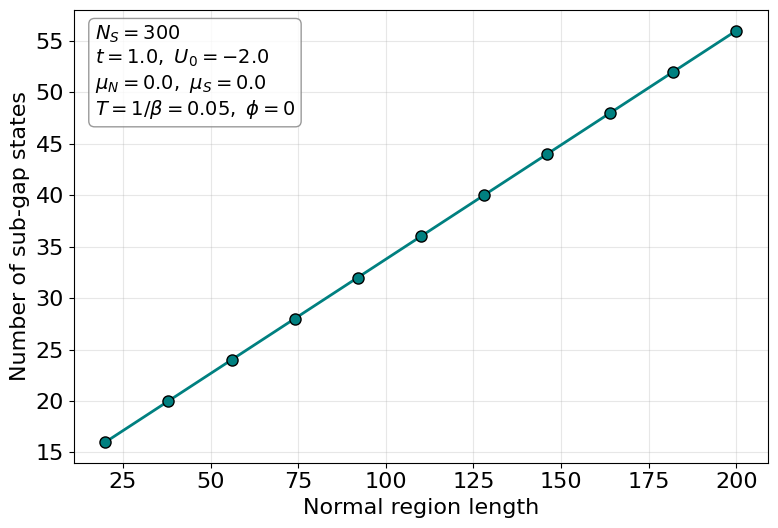
\includegraphics[width=0.6\textwidth]{figures/ch6_number_of_bound_states.png}   
    \caption{Number of Andreev bound states depending on the length of the junction.}
    \label{fig:nb_ABS_vs_L}
\end{figure}


\subsection{Short-junction limit}

When the normal region is much shorter than the superconducting coherence length $\xi_0 = \hbar v_F / |\Delta|$, the phase accumulated by a quasiparticle traversing the junction is small,
\[
  \delta k\, L = \frac{E L}{\hbar v_F} \ll 1 .
\]
Neglecting this term, Eq.~\eqref{eq:ABS_quantization} simplifies dramatically.  We find the two solutions
\begin{equation}
  \boxed{
  E_{\pm}(\Delta\phi) = \pm |\Delta| \cos\!\left(\frac{\Delta\phi}{2}\right) .
  }
  \label{eq:ABS_short}
\end{equation}
These are the Andreev bound states of a clean short junction.

\subsubsection{Continuum contribution}

The Josephson current is carried not only by the discrete bound states but also by the continuum of states with $|E|>|\Delta|$.  In an SNS junction the continuum spectrum is also phase-dependent and can contribute significantly to the supercurrent, especially at finite temperature and for $L \gtrsim \xi_0$.  However, Beenakker~\cite{beenaker_1992} has shown that in the limit $L \ll \xi_0$ the continuum contribution cancels exactly, leaving only the bound-state current. We can therefore use formula~\eqref{eq:I_from_spectrum} for short junctions using only the bound-states.

\subsubsection{Josephson current from the bound states}

The supercurrent carried by a bound state is, 
\begin{equation}
  I(\phi) = \frac{2e}{\hbar} \sum_{n} \frac{d E_n}{d\phi} f(E_n) .
  \label{eq:current_ABS_general}
\end{equation}
For a short ballistic junction, we get
\begin{equation}
  \boxed{
  I(\phi,T) = \frac{e|\Delta|}{\hbar} \sin\!\left(\frac{\phi}{2}\right)
              \tanh\!\left( \frac{|\Delta|}{2k_B T} \cos\!\left(\frac{\phi}{2}\right) \right) .
  }
  \label{eq:CPR_KO_T}
\end{equation}
At $T=0$ the CPR has a forward skewness with maximum at $\phi=\pi$, while at $T>0$ the cusp is rounded and the maximum shifts toward $\phi=\pi/2$.

\subsubsection{Comparison with numerical simulations}

Figure~\ref{fig:ABS_comparisons} shows the CPR features obtained numerically for three cases: a short transparent junction, a long transparent junction, and a short junction with a Fermi-wavevector mismatch.

\begin{figure}[H]
  \centering
  \begin{subfigure}[b]{0.32\textwidth}
    \centering
    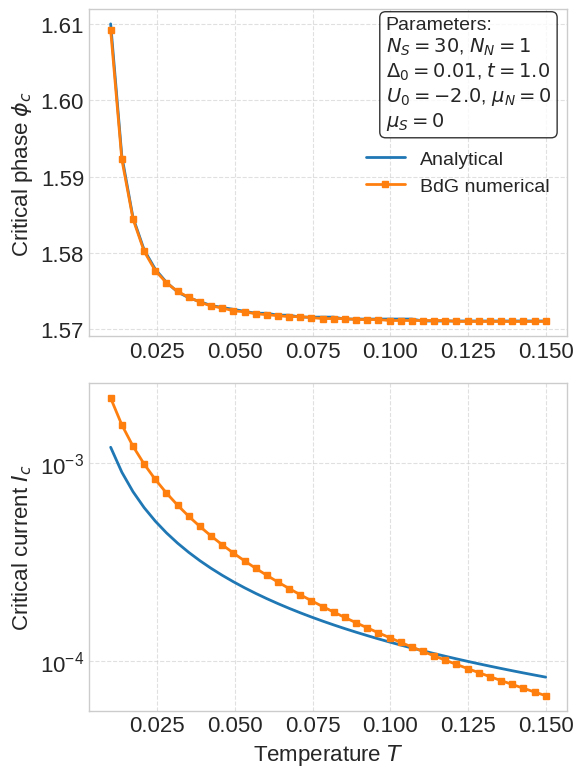
\includegraphics[width=\textwidth]{figures/ch6_short_junction_theory_short_ballistic.png}
    \caption{Short transparent junction.}
    \label{fig:short_clean}
  \end{subfigure}
  \hfill
  \begin{subfigure}[b]{0.32\textwidth}
    \centering
    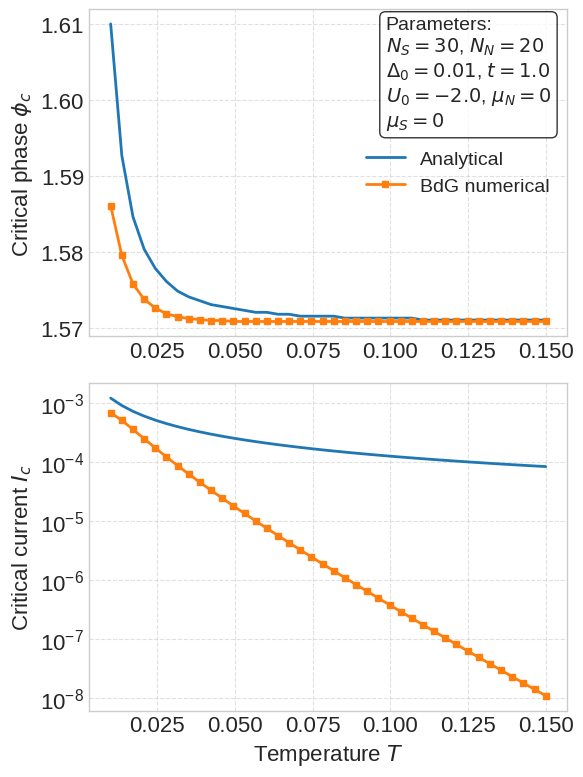
\includegraphics[width=\textwidth]{figures/ch6_short_junction_theory_long.png}
    \caption{Long transparent junction.}
    \label{fig:long_clean}
  \end{subfigure}
  \hfill
  \begin{subfigure}[b]{0.32\textwidth}
    \centering
    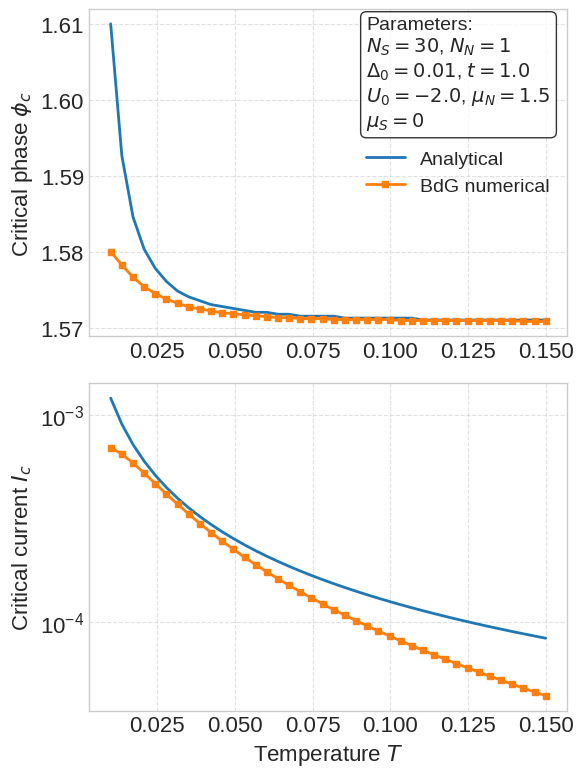
\includegraphics[width=\textwidth]{figures/ch6_short_junction_theory_short_mismatch.png}
    \caption{Short mismatched junction.}
    \label{fig:short_diff}
  \end{subfigure}
  \caption{
    Numerical current-phase relations compared with the analytical ballistic short-junction formula.}
  \label{fig:ABS_comparisons}
\end{figure}

For a short, transparent junction (Fig.~\ref{fig:short_clean}), the numerical critical phase tracks the analytical prediction with remarkable fidelity. This agreement directly confirms the Andreev-bound-state
picture: a single pair of sub-gap states, carries the entire Josephson current.  The overall shape of $I(\phi)$ follows the analytical prediction with some deviations that probably arise from the fixed-phase-in-leads condition used in the one-shot diagonalization (Section~\ref{sec:square_well_method}). Since the phase is forced to be flat inside the superconductors, the supercurrent cannot be sustained in
those regions. Therefore the solution is not current-conserving along the whole chain.

The second panel (Fig.~\ref{fig:long_clean}) illustrates the long-junction regime ($L \gtrsim \xi_0$).  Here the normal region hosts many Andreev levels, and the continuum of states above the gap begins to contribute significantly to the supercurrent. The critical current is reduced, and the forward skewness of the short junction is reduced. The analytical formula derived for a single pair of bound states is no longer adequate.

The third panel (Fig.~\ref{fig:short_diff}) addresses the effect of a Fermi-wavevector mismatch ($\mu_N \neq \mu_S$).  Although the junction is physically short, normal reflections appear at the NS interfaces: an electron incident from the normal side can be reflected as an electron rather than being Andreev-converted into a hole. This reduces the effective transparency $\mathcal{T}$ of the junction and reshapes the Andreev-bound-state spectrum. The CPR deviates from the analytical curve. To capture these effects quantitatively one must replace the perfect-transparency assumption by a scattering-matrix formalism that handles arbitrary transmission probabilities. This is the subject of the next section.


\section{Short junction with finite transparency}
\label{sec:Beenakker}
\subsection{Direct inclusion of a Fermi-wavevector mismatch}

In the Andreev-bound-state derivation for short transparent junction we assumed identical Fermi wavevectors in the normal and superconducting regions, $k_{F,N}=k_{F,S}=k_F$. This assumption guaranteed perfect Andreev reflection at every N-S interface: an electron is converted into a hole with unit probability. Realistic junctions, however, are often made of different materials or have different carrier densities, so $k_{F,N}\neq k_{F,S}$. A natural first attempt to
incorporate this mismatch is to re-derive the Andreev scattering matrices with different wavevectors on the two sides of an interface.

Consider a single N-S interface at $x=0$ with $\Delta(x)=|\Delta|e^{\mathrm{i}\phi}$ for $x>0$ and
$\Delta=0$ for $x<0$. The wavefunctions on the normal and superconducting side are given by Eq.~\eqref{eq:Psi_NS} where the Fermi-wavevectors are $k_{F,N}$ in the normal region and $k_{F,S}$ in the superconducting region.

Matching the wavefunction and its derivative and neglecting $\delta k$ and $\kappa$ leads to a modified set of linear equations. Defining the wavevector ratio
\begin{equation}
  u \equiv \frac{k_{F,N}}{k_{F,S}},
\end{equation}
the matching conditions become
\begin{equation}
  \begin{cases}
    1 + r_{ee} = \Delta\,(t_1 + t_2), \\
    r_{eh}    = (E - \mathrm{i}\Omega)\,t_1 + (E + \mathrm{i}\Omega)\,t_2, \\
    u\,(1 - r_{ee}) = \Delta\,(t_1 - t_2), \\
    u\,r_{eh} = (E - \mathrm{i}\Omega)\,t_1 - (E + \mathrm{i}\Omega)\,t_2 .
  \end{cases}
  \label{eq:matching_u}
\end{equation}
Solving for the reflection amplitudes yields
\begin{equation}
  \boxed{
  \begin{aligned}
    r_{ee} &= r_{hh} = \frac{-\mathrm{i}\Omega\,(1-u^2)}{2uE + \mathrm{i}\Omega\,(1+u^2)}, \\[4pt]
    r_{eh} &= \frac{2u\,\Delta^*}{2uE + \mathrm{i}\Omega\,(1+u^2)}, \qquad
    r_{he} = \frac{2u\,\Delta}{2uE + \mathrm{i}\Omega\,(1+u^2)} .
  \end{aligned}}
  \label{eq:reflection_u}
\end{equation}
When $u=1$ we recover $r_{ee}=0$ and $|r_{eh}|=1$. For $u\neq1$ a finite normal reflection appears. The corresponding Andreev scattering matrices at the right and left interfaces are
\begin{equation}
  S_R(E) = \frac{1}{2uE+\mathrm{i}\Omega(1+u^2)}
            \begin{pmatrix}
              -\mathrm{i}\Omega(1-u^2) & 2u|\Delta|\,e^{\mathrm{i}\phi_R} \\[2pt]
              2u|\Delta|\,e^{-\mathrm{i}\phi_R} & -\mathrm{i}\Omega(1-u^2)
            \end{pmatrix},
  \label{eq:S_R_u}
\end{equation}
\begin{equation}
  S_L(E) = \frac{1}{2uE+\mathrm{i}\Omega(1+u^2)}
            \begin{pmatrix}
              -\mathrm{i}\Omega(1-u^2) & 2u|\Delta|\,e^{\mathrm{i}\phi_L} \\[2pt]
              2u|\Delta|\,e^{-\mathrm{i}\phi_L} & -\mathrm{i}\Omega(1-u^2)
            \end{pmatrix}.
  \label{eq:S_L_u}
\end{equation}


\subsubsection{Bound-state condition for a zero-length junction}

If we apply these new scattering matrices to a junction of zero normal length, $L \rightarrow0$, there is no propagation, and the round-trip matrix
is simply the product
\begin{equation}
  M = S_L S_R .
  \label{eq:M_zero}
\end{equation}
A straightforward multiplication of the matrices~\eqref{eq:S_R_u} and~\eqref{eq:S_L_u} gives
\begin{equation}
  M = \frac{1}{(2uE+\mathrm{i}\Omega(1+u^2))^2}
      \begin{pmatrix}
        -\Omega^2(1-u^2)^2 + 4u^2|\Delta|^2 e^{-\mathrm{i}\Delta\phi} &
        -2\mathrm{i}u\Omega(1-u^2)|\Delta|(e^{\mathrm{i}\phi_R}+e^{\mathrm{i}\phi_L}) \\[6pt]
        -2\mathrm{i}u\Omega(1-u^2)|\Delta|(e^{-\mathrm{i}\phi_R}+e^{-\mathrm{i}\phi_L}) &
        -\Omega^2(1-u^2)^2 + 4u^2|\Delta|^2 e^{\mathrm{i}\Delta\phi}
      \end{pmatrix}.
  \label{eq:M_explicit}
\end{equation}
The bound-state condition $\det(M-\mathbb{I})=0$ remarkably simplifies to
\begin{equation}
  E = \pm |\Delta| \cos\!\left(\frac{\Delta\phi}{2}\right),
  \label{eq:ABS_same}
\end{equation}
exactly the same spectrum as in the perfectly transparent case. According to this result, a Fermi-wavevector mismatch does not alter the Andreev levels at all.

The paradox arises because by setting $L=0$ we not only eliminated the propagation phase across the normal region, but we also canceled all effects of the wavevector mismatch on the normal reflection amplitudes.  In a junction of finite length the mismatch does influence both the propagation phases (because electrons and holes travel with different wavevectors) and the interface scattering. Taking $L\to0$ removes both effects simultaneously, which is why the naive calculation yielded the same bound-state spectrum as the perfectly matched case.

A consistent treatment must separate the length scales: the rapid Fermi-wavelength oscillations should be neglected, while the Andreev reflections at the SN boundaries should be kept. In practice this means that we describe the whole normal part of the junction by a normal-state scattering matrix $s_0$. The Fermi-wavevector mismatch then enters solely through the transmission eigenvalues of $s_0$, and its effect on the Andreev bound-state spectrum is fully captured. This is the essence of the scattering-matrix formalism introduced by Beenakker~\cite{beenaker_1992}, which we outline below.



\subsection{Beenakker’s scattering-matrix formalism}

Consider a normal metal (length $L$, possibly with disorder or a chemical-potential mismatch) connected to two ideal superconductors via maximally transparent contacts. The normal region is described by a unitary scattering matrix $s_0(E)$ for electron excitations. In the basis of right- and left-moving electrons at the two contacts,
\begin{equation}
  s_0(E) = \begin{pmatrix}
    r_{11} & t_{12} \\
    t_{21} & r_{22}
  \end{pmatrix},
  \label{eq:s0}
\end{equation}
where $r_{ij}$ and $t_{ij}$ are reflection and transmission amplitudes.  The full SNS
junction is then modeled by augmenting $s_0$ with Andreev reflection matrices that couple
electrons and holes at the SN interfaces.  In the short-junction limit $L\ll\xi_0$,
Beenakker showed that the sub-gap Andreev bound states are determined by the eigenvalues
$\mathcal{T}_p$ ($p=1,\dots,N$) of the transmission matrix product $t_{12}t_{12}^\dagger$.
Specifically, the bound-state energies are
\begin{equation}
  E_p(\phi) = \Delta_0 \sqrt{1 - \mathcal{T}_p \sin^2(\phi/2)} .
  \label{eq:Beenakker_ABS}
\end{equation}
The corresponding Josephson current is
\begin{equation}
  I(\phi) = \frac{e\Delta_0}{2\hbar} \sum_{p=1}^N
            \frac{\mathcal{T}_p \sin\phi}{\sqrt{1 - \mathcal{T}_p \sin^2(\phi/2)}} \,
            \tanh\!\left( \frac{\Delta_0}{2k_B T} \sqrt{1 - \mathcal{T}_p \sin^2(\phi/2)} \right).
  \label{eq:Beenakker_current_general}
\end{equation}

\subsection{One-dimensional single-channel case}

Our tight-binding chain is strictly one-dimensional, so there is only one propagating channel ($N=1$).  The transmission probability $\mathcal{T}$ of this channel is all that is needed. If the normal region has a chemical potential $\mu_N$ different from that of the superconductors ($\mu_S$), the corresponding Fermi wavevectors are
\begin{equation}
  k_{F,N} = \frac{1}{a}\arccos\!\left(-\frac{\mu_N}{2t}\right), \qquad
  k_{F,S} = \frac{1}{a}\arccos\!\left(-\frac{\mu_S}{2t}\right).
  \label{eq:mu}
\end{equation}
The normal-region scattering matrix $s_0$ is obtained by matching plane waves at the two
interfaces, as detailed in the previous subsection but now consistently treating the whole
normal part as a separate entity placed between ideal NS boundaries. Matching the wavefunctions at the interface \(-L/2\) and \(L/2\) we get

\[\begin{cases}
    c_e^+(N_1)e^{-\mathrm{i}Lk_{F,S}/2}+c_e^-(N_1)e^{\mathrm{i}Lk_{F,S}/2}=c_e^+(N)e^{-\mathrm{i}Lk_{F,N}/2}+c_e^-(N)e^{\mathrm{i}Lk_{F,N}/2}\\
    k_{F,S}(c_e^+(N_1)e^{-\mathrm{i}Lk_{F,S}/2}-c_e^-(N_1)e^{\mathrm{i}Lk_{F,S}/2})=k_{F,N}(c_e^+(N)e^{-\mathrm{i}Lk_{F,N}/2}+c_e^-(N)e^{\mathrm{i}Lk_{F,N}/2})\\
    c_e^+(N)e^{\mathrm{i}Lk_{F,N}/2}+c_e^-(N)e^{-\mathrm{i}Lk_{F,N}/2}=c_e^+(N_2)e^{\mathrm{i}Lk_{F,S}/2}+c_e^-(N_2)e^{-\mathrm{i}Lk_{F,S}/2} \\
    k_{F,N}(c_e^+(N)e^{\mathrm{i}Lk_{F,N}/2}-c_e^-(N)e^{-\mathrm{i}Lk_{F,N}/2})=k_{F,S}(c_e^+(N_2)e^{\mathrm{i}Lk_{F,S}/2}-c_e^-(N_2)e^{-\mathrm{i}Lk_{F,S}/2})
\end{cases}\]
The normal-region scattering matrix is found to be
\begin{equation}
  s_0 = \frac{1}{D}
        \begin{pmatrix}
          (k_{F,N}^2 - k_{F,S}^2) \sin(k_{F,N}L) &
          2 k_{F,N} k_{F,S} \, e^{-\mathrm{i} k_{F,S}L} \\[6pt]
          2 k_{F,N} k_{F,S} \, e^{-\mathrm{i} k_{F,S}L} &
          (k_{F,N}^2 - k_{F,S}^2) \sin(k_{F,N}L)
        \end{pmatrix},
  \label{eq:s0_mismatch}
\end{equation}
where
\begin{equation}
  D = 2 k_{F,N} k_{F,S} \cos(k_{F,N}L) - \mathrm{i}\,(k_{F,N}^2 + k_{F,S}^2) \sin(k_{F,N}L).
\end{equation}
The transmission probability is therefore
\begin{equation}
  \boxed{
  \mathcal{T} = |t_{12}|^2 = \frac{4k_{F,N}^2 k_{F,S}^2}
                        {4k_{F,N}^2 k_{F,S}^2
                         + (k_{F,N}^2 - k_{F,S}^2)^2 \sin^2(k_{F,N} L)}
    = \left[ 1 + \frac{(k_{F,N}^2 - k_{F,S}^2)^2}{4k_{F,N}^2 k_{F,S}^2}
                 \sin^2(k_{F,N} L) \right]^{-1} .
  }
  \label{eq:T_mismatch}
\end{equation}

The current becomes
\begin{equation}
\boxed{
I(\phi) = \frac{e\Delta_0}{2\hbar} \frac{\mathcal{T} \sin\phi}{\sqrt{1 - \mathcal{T} \sin^2(\phi/2)}} \,
\tanh\!\left( \frac{\Delta_0}{2k_B T} \sqrt{1 - \mathcal{T} \sin^2(\phi/2)} \right). 
}\label{eq:Beenakker_current}
\end{equation}
For matched Fermi wavevectors ($k_{F,N}=k_{F,S}$) Eq.~\eqref{eq:T_mismatch} gives $\mathcal{T}=1$, and the Beenakker formula~\eqref{eq:Beenakker_current} reduces to the ballistic short-junction CPR.  For a finite mismatch the transmission is lowered. In the tunnel limit ($\mathcal{T}\ll 1$) the CPR reduces to \(I \propto \sin\phi\), with a critical current proportional to $\mathcal{T}$.

For intermediate transmissions, the CPR smoothly interpolates between these two
extremes.  At finite temperature the sharp cusp at $\phi=\pi$ is rounded and the
maximum shifts toward $\pi/2$, an effect already present in the ballistic case.
Figure~\ref{fig:cpr_finite_T} illustrates this dependence for a representative
temperature $k_B T = 0.1\,\Delta_0$.

\begin{figure}[H]
  \centering
  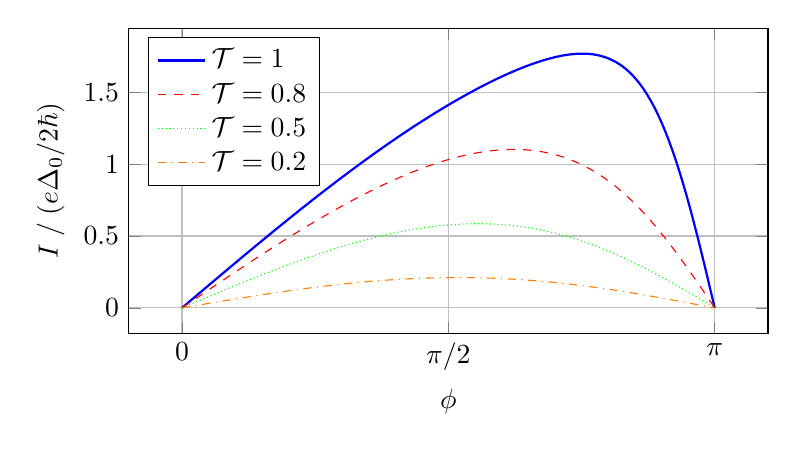
\begin{tikzpicture}
    \begin{axis}[
        width=0.80\textwidth,
        height=0.45\textwidth,
        xlabel=$\phi$,
        ylabel={$I\;/\;(e\Delta_0/2\hbar)$},
        legend pos=north west,
        domain=0:pi,
        samples=150,
        grid=major,
        xtick={0,pi/2,pi},
        xticklabels={$0$,$\pi/2$,$\pi$},
        ytick={0,0.5,1,1.5},
        legend cell align=left
      ]
      % define temperature parameter
      \pgfmathsetmacro{\kT}{0.1}
      % T=1: ballistic
      \addplot [blue, thick] {2*sin(deg(x/2))*tanh( cos(deg(x/2))/(2*\kT) )};
      \addlegendentry{$\mathcal{T}=1$};

      % T=0.8
      \addplot [red, dashed] {0.8*sin(deg(x))/sqrt(1 - 0.8*(sin(deg(x/2)))^2)
            * tanh( sqrt(1 - 0.8*(sin(deg(x/2)))^2) / (2*\kT) ) };
      \addlegendentry{$\mathcal{T}=0.8$};

      % T=0.5
      \addplot [green, densely dotted] {0.5*sin(deg(x))/sqrt(1 - 0.5*(sin(deg(x/2)))^2)
            * tanh( sqrt(1 - 0.5*(sin(deg(x/2)))^2) / (2*\kT) ) };
      \addlegendentry{$\mathcal{T}=0.5$};

      % T=0.2
      \addplot [orange, dashdotted] {0.2*sin(deg(x))/sqrt(1 - 0.2*(sin(deg(x/2)))^2)
            * tanh( sqrt(1 - 0.2*(sin(deg(x/2)))^2) / (2*\kT) ) };
      \addlegendentry{$\mathcal{T}=0.2$};
    \end{axis}
  \end{tikzpicture}
  \caption{CPR for a short single-channel SNS junction at finite temperature ($k_B T = 0.1\,\Delta_0$) for various transparencies $\mathcal{T}$, according to the Beenakker formula~\eqref{eq:Beenakker_current}.}
  \label{fig:cpr_finite_T}
\end{figure}

The critical current decreases with $\mathcal{T}$, and the skewness shifts from values above $\pi/2$ toward $\pi/2$ as the transmission is reduced.  These features are fully consistent with the numerical self-consistent results presented in Chapter~5, where a mismatch in $\mu_N$ was seen to lower the critical current and bring the skewness closer to $\pi/2$.


\subsection{Comparison of the Beenakker formula with numerical simulations}

We now compare directly the analytical CPR with the numerical BdG simulation for a mismatched short junction. Figure~\ref{fig:comparison_models_mismatch} shows three curves: the purely ballistic formula ($\mathcal{T}=1$), the Beenakker curve with $\mathcal{T}$ computed from Eq.~\eqref{eq:T_mismatch}, and the numerical
result.

\begin{figure}[H]
  \centering 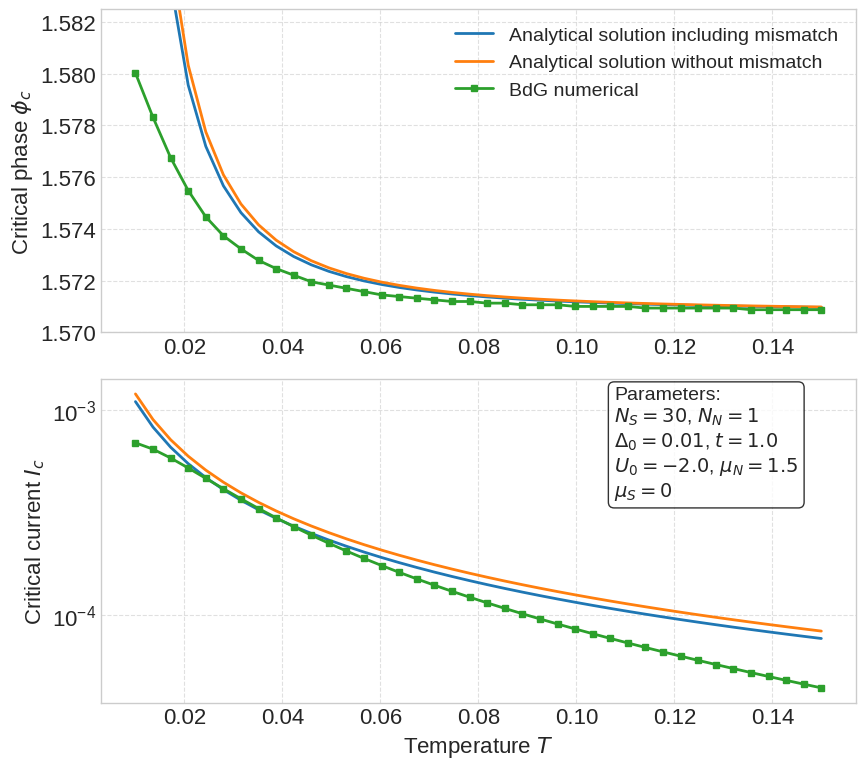
\includegraphics[width=0.65\textwidth]{figures/ch6_beenakker_mismatch.png}
  \caption{Comparison of analytical CPRs features with the fixed-gap BdG result for a
    short mismatched junction.}
  \label{fig:comparison_models_mismatch}
\end{figure}

The Beenakker curve with the mismatch-derived transmission brings the CPR closer to the numerical data, capturing the reduced critical current and the shift of the maximum toward $\pi/2$.  However a significant discrepancy remains, which can be attributed to the approximations made in the formula for the chemical potential Eq.~(\eqref{eq:mu}) used to compute $\mathcal{T}$.  Despite these quantitative differences, the scattering-matrix approach provides a description of the crossover from ballistic to tunnel transport and correctly identifies the reduction of the effective transparency as the key mechanism responsible for the changes in the CPR observed in the simulations.

\section{Fabry-Pérot resonances and oscillations in the critical current and phase}
\label{sec:FabryPerot}
The transmission probability of the normal region, derived in
Sec.~\ref{sec:Beenakker} for a single-channel junction, is
\begin{equation}
  \mathcal{T}(\mu_N,\mu_S) = \left[\, 1 + \frac{(k_{F,N}^2 - k_{F,S}^2)^2}{4k_{F,N}^2 k_{F,S}^2}\,
               \sin^2(k_{F,N} L) \right]^{-1},
  \label{eq:T_mismatch_osc}
\end{equation}
with $k_{F,N} = \frac{1}{a}\arccos(-\mu_N/2t)$ and $k_{F,S}$ defined analogously. The $\sin^2$ term arises from the interference of electron waves that are partially reflected at the two N-S interfaces.  When the round-trip phase accumulated in the normal region is an integer multiple of $\pi$,
\begin{equation}
  k_{F,N} L = \pi m,
  \label{eq:FP_condition}
\end{equation}
the factor $\sin(k_{F,N}L)$ vanishes and the transmission reaches unity $\mathcal{T}=1$, regardless of the mismatch. Equation~\eqref{eq:FP_condition} is precisely the Fabry-Pérot constructive interference condition~\cite{sahu_fabryperot_2023, rittenhouse_fabry-perot_1994}. Away from these resonances, $T$ is suppressed, with the suppression growing as the mismatch $|k_{F,N}-k_{F,S}|$ increases.

Since the Josephson current in the short-junction limit is given by the Beenakker
formula~\eqref{eq:Beenakker_current}
\begin{equation}
  I(\phi) = \frac{e\Delta_0}{2\hbar}\,
            \frac{\mathcal{T}\sin\phi}{\sqrt{1 - \mathcal{T}\sin^2(\phi/2)}}\,
            \tanh\!\left( \frac{\Delta_0}{2k_B T} \sqrt{1 - \mathcal{T}\sin^2(\phi/2)} \right),
  \label{eq:Beenakker_current_osc}
\end{equation}
any oscillation in $\mathcal{T}$ directly translates into oscillations of the CPR, and consequently of the critical current $I_{\max}$ and of the skewness $\phi_{\max}$.

This resonant behavior is exactly what we observed numerically in Figs.~\ref{fig:crit_muN_short} and~\ref{fig:crit_muN_long_FPL}: the critical current exhibits small but distinct oscillations as a function of $\mu_N$, and the skewness shows corresponding modulations.  At low temperature the resonance peaks are sharp because the Andreev bound-state energy $E(\phi) = \Delta_0\sqrt{1-\mathcal{T}\sin^2(\phi/2)}$ touches zero at $\phi=\pi$ when $\mathcal{T}=1$, leading to a cusp in $I(\phi)$ and a singularity in $\partial E/\partial\phi$.

\begin{figure}[H]
  \centering 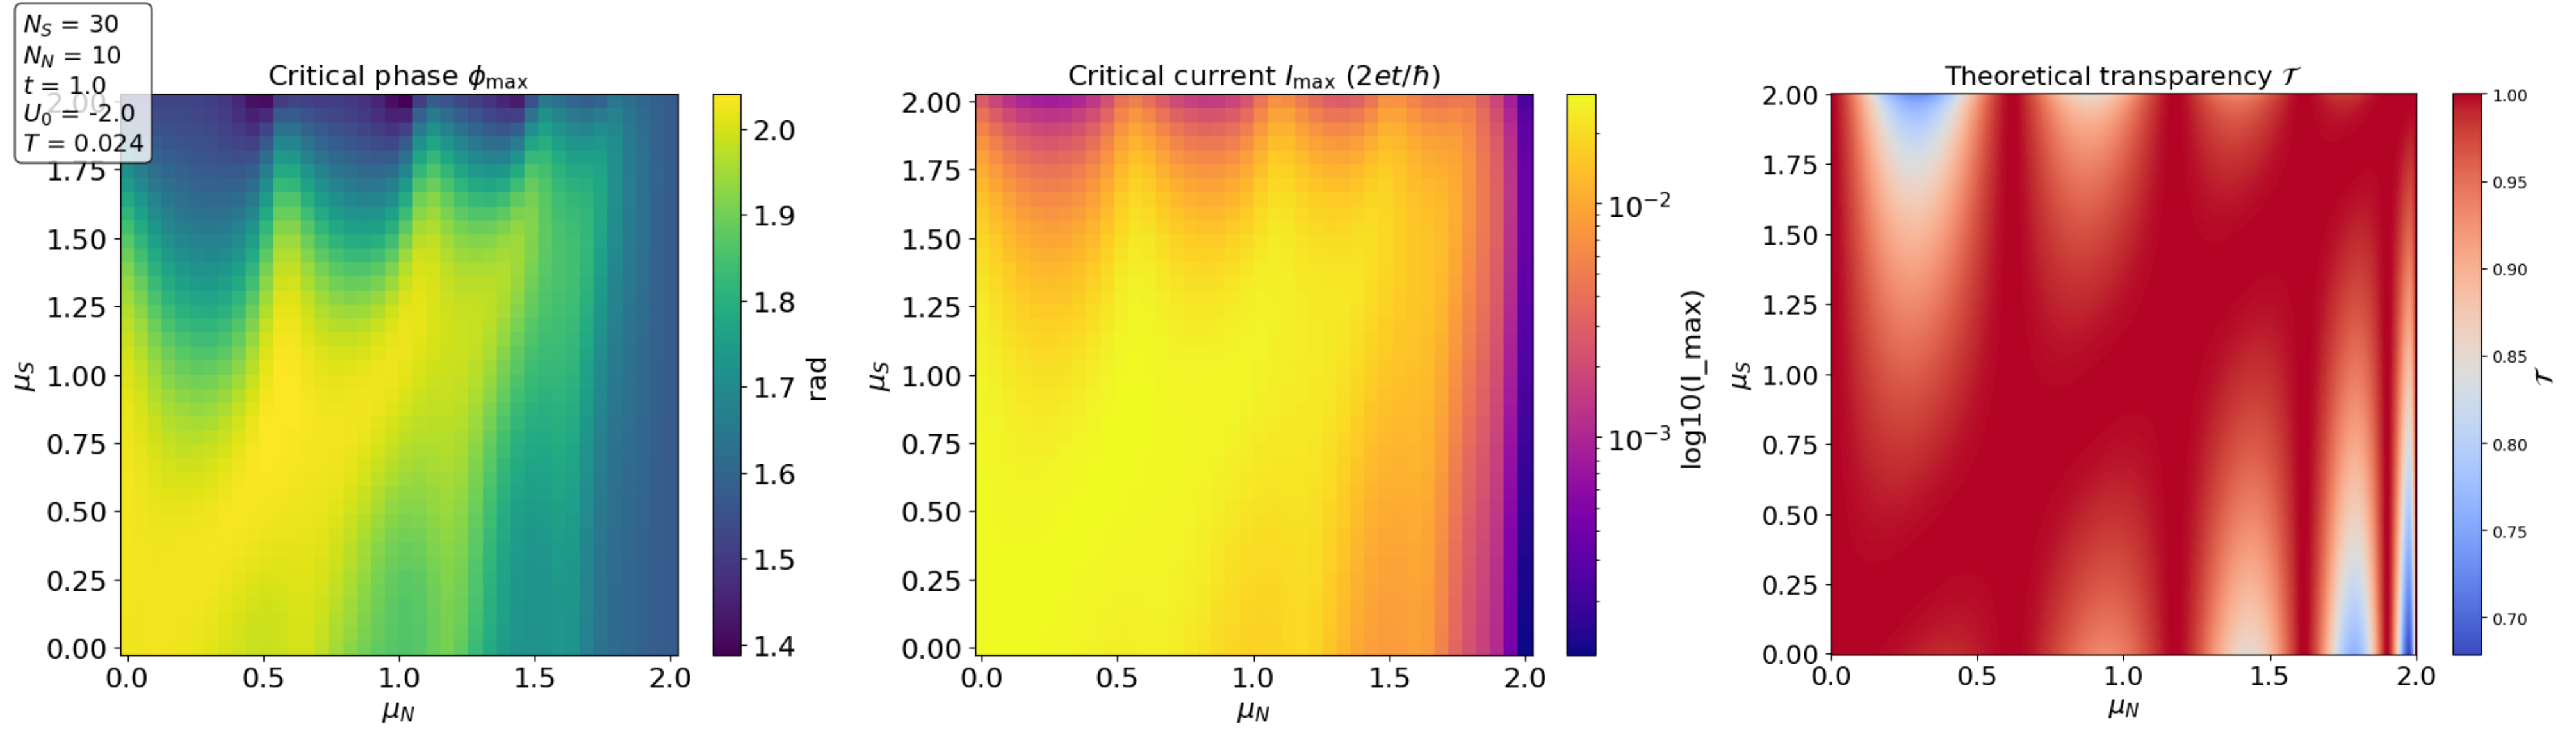
\includegraphics[width=0.95\textwidth]{figures/ch6_transmission_vs_critical_map.png}
  % (replace with your actual numerical comparison plot)
  \caption{Analytical transparency and numerical critical current and phase.}
  \label{fig:transmittance}
\end{figure}

We compare the analytical transparency with numerical results for critical current and phase as functions of $\mu_N$ and $\mu_S$ in Fig.~\ref{fig:transmittance}. Excellent agreement is found between the modulations of the analytical transparency and the position of the resonances of the critical current and phase. This confirms that the single‑channel Beenakker formula, combined with the Fabry‑Pérot condition, well describes the effect of Fermi‑wavevector mismatch in short SNS junctions.


\chapter{Long ballistic junctions}

In Chapter~6 we studied short SNS junctions, where the normal region is much shorter than the superconducting coherence length \(\xi_0 = \hbar v_F / \Delta_0\) and the Josephson current is carried by a single pair of Andreev bound states.  When the junction length \(L\) becomes comparable to or larger than \(\xi_0\) the normal region accommodates many Andreev levels, which for \(L \gg \xi_0\) merge into a quasi-continuous spectrum.  Moreover, the continuum of states with \(|E| > \Delta_0\) contributes significantly to the supercurrent, and the simple two-level picture of the short junction breaks down.

In this chapter we extend the analysis to long ballistic SNS junctions.  We start from the exact bound-state~\eqref{eq:ABS_quantization} and discuss how it leads to a dense spectrum of Andreev levels.  We then present the Ishii formula~\cite{ishii_josephson_1970} for the current-phase relation at zero temperature, and we compare it with our numerical tight-binding simulations.

\section{From discrete to continuous Andreev spectrum}

For a one-dimensional ballistic SNS junction of length \(L\), the bound-state condition was derived in Eq.~\eqref{eq:ABS_quantization}:
\begin{equation}
  \arccos\!\left(\frac{E}{\Delta_0}\right) = \pm \frac{\Delta\phi}{2} + \frac{E L}{\hbar v_F} + m\pi, \qquad m \in \mathbb{Z}.
  \label{eq:long_ABS}
\end{equation}
Here \(\Delta\phi = \phi_R - \phi_L\) is the phase difference, and we have assumed identical superconducting gaps \(\Delta_0\) on both sides.  The term \(E L / \hbar v_F\) describes the phase accumulated by a quasiparticle while traversing the normal region.  

When \(L \ll \xi_0\), this phase is negligible and one recovers the short-junction spectrum \(E_{\pm} = \pm \Delta_0 \cos(\Delta\phi/2)\).  For longer junctions, however, the phase factor cannot be ignored.  For any given \(\Delta\phi\) there may be several integer values of \(m\) that yield solutions with \(|E| < \Delta_0\), i.e.\ multiple bound states.  As \(L / \xi_0\) increases, these levels become denser, and eventually for \(L \gg \xi_0\) they form a quasi-continuous band inside the gap.  At the same time, the continuum states (\(|E| > \Delta_0\)) acquire a phase dependence and contribute to the Josephson current.

\section{The Ishii formula}

A complete calculation of the Josephson current in a clean, one-dimensional long SNS junction at zero temperature, taking into account both the bound states and the continuum, was carried out by Ishii~\cite{ishii_josephson_1970} and by Kulik~\cite{kulik_macroscopic_1969} by a Green's-function method. The current-phase relation becomes strictly linear,
\begin{equation}
  \boxed{ I(\phi) = \frac{e v_F}{\pi L}\,\Delta\phi, \qquad |\Delta\phi| < \pi, }
  \label{eq:Ishii}
\end{equation}
and periodically extended with period \(2\pi\) outside this interval, giving a sawtooth shape. This linear dependence is a direct consequence of the cancellation between the bound-state and continuum contributions: the continuum carries a current that opposes the bound-state current, and the net result is simply proportional to the phase difference.

Equation~\eqref{eq:Ishii} shows that the critical current decays inversely with the junction length in the perfectly transparent limit at zero temperature. Moreover the skewness is maximal and the shape is a sawtooth rather than the \(\sin(\phi/2)\) of the short ballistic case.

\section{Numerical simulations of long ballistic junctions}

We now test the Ishii prediction against our self-consistent tight-binding BdG solver.  We consider a junction with \(N_N = 30\) normal sites, the CPR is shown in Fig.~\ref{fig:long_cpr}.


\begin{figure}[H]
  \centering
  \begin{subfigure}[b]{0.48\textwidth}
    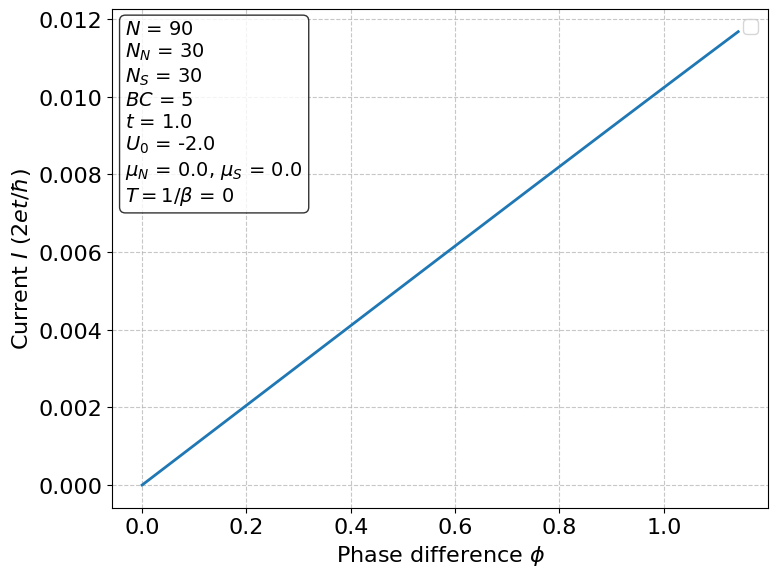
\includegraphics[width=\textwidth]{figures/ch7_sawtooth_fpb.png}
    \caption{FPB.}
    \label{fig:sawtooth cpr ishii FPB}
  \end{subfigure}
  \hfill
  \begin{subfigure}[b]{0.48\textwidth}
    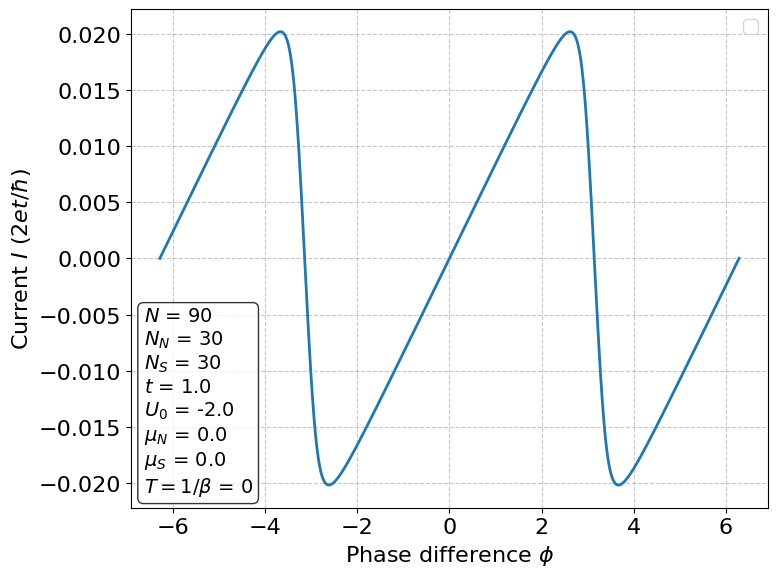
\includegraphics[width=\textwidth]{figures/ch7_sawtooth_fpl.png}
    \caption{FPL.}
    \label{fig:sawtooth cpr ishii FPL}
  \end{subfigure}
  \caption{Numerical CPR for a long, fully transparent SNS junction with $N_N=30$ at $T=0$.}
  \label{fig:long_cpr}
\end{figure}



The data points follow the straight line over the entire reachable phase interval for the FPB method. The FPL method allows reaching higher phase difference and we can clearly see the sawtooth shape of the CPR.




\subsection{Contribution of the continuum states}

To understand why the net current in a long junction settles on the simple sawtooth form~\eqref{eq:Ishii}, it is instructive to separate the total current into the contributions from the Andreev bound states ($|E|<\Delta_0$) and from
the continuum ($|E|>\Delta_0$). In the long-junction limit the continuum contribution becomes non negligible. Remarkably, the two contributions almost cancel each other: the bound states produce a current of one sign, while the continuum states carry a current of opposite sign. The total sum, however, is precisely the linear sawtooth~\eqref{eq:Ishii}.

Figure~\ref{fig:continuum_compensation} illustrates this cancellation for a very long junction with $N_N = 300$.

\begin{figure}[H]
  \centering
  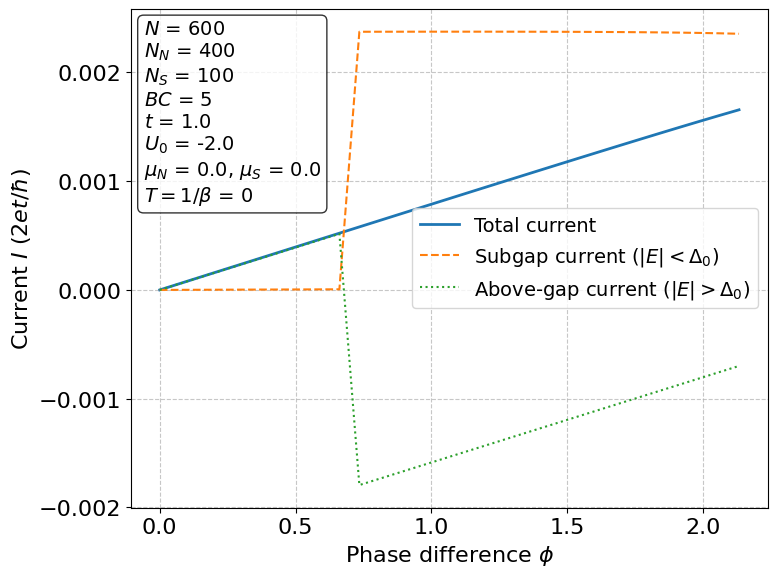
\includegraphics[width=0.50\textwidth]{figures/ch7_continuum_compensation.png}
  \caption{Decomposition of the Josephson current into bound-state and continuum contributions for a long ballistic junction (FPB).}
  \label{fig:continuum_compensation}
\end{figure}


The bound-state current alone is not a sawtooth. It has a complex
shape which is compensated by the continuum current that has approximately the same amplitude as the bound-state current but the opposite. When the two are added, they cancel almost completely, leaving a perfect linear dependence that closely follows the Ishii formula. This has been explored by Thuneberg~\cite{thuneberg_square-well_2024}.


\subsection{Length dependence of the CPR slope}

The Ishii formula~\eqref{eq:Ishii} predicts a strictly linear CPR at zero
temperature, so that the slope $\mathrm{d}I/\mathrm{d}\phi\big|_{\phi=0}
= e v_F / (\pi L)$ is inversely proportional to the junction length. To test this prediction we therefore extract the linear slope
of the CPR near $\phi = 0$ for a set of junction lengths while keeping all other parameters fixed. The results are plotted in Fig.~\ref{fig:long_ic_vs_L} on a log-log scale.

\begin{figure}[H]
  \centering
  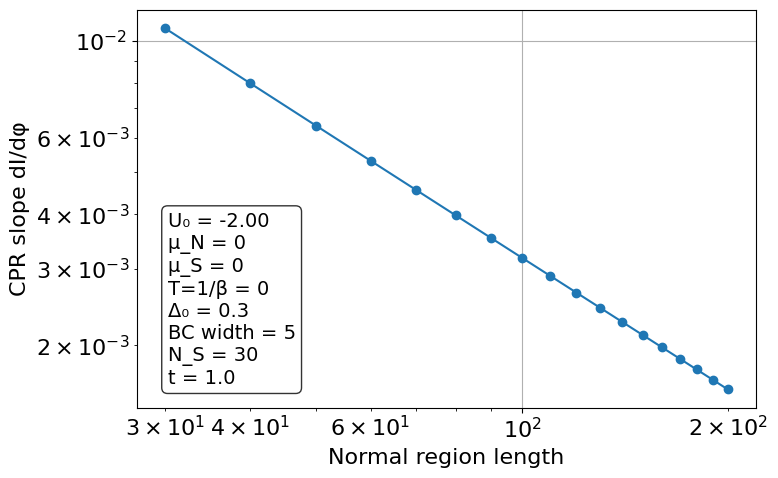
\includegraphics[width=0.5\textwidth]{figures/ch7_slope_vs_length.png}
  \caption{Slope of the linear CPR as a function of normal-region length $L = N_N a$.}
  \label{fig:long_ic_vs_L}
\end{figure}



The slope of the data points is proportional to $1/L$ for all lengths studied, demonstrating the expected behavior.

\subsection{Finite-temperature effects}

At non-zero temperature, the sharp sawtooth becomes rounded, and the critical current decreases.  A  study of the temperature dependence was already presented in Chapter~5 for a transparent junction of length $N_N=30$. There we observed that the CPR evolves from a forward-skewed (nearly linear) shape at low $T$ to a more sinusoidal shape as $T$ approaches $T_c$, with the critical current decaying exponentially. These observations are consistent with the theoretical expectations for long junctions and confirm that the numerical model captures both the zero-temperature ballistic limit and the thermal smearing correctly.








\chapter{Conclusion}

In this work we have developed and applied a fully self-consistent tight-binding Bogoliubov-de Gennes (BdG) framework to study the properties of one-dimensional s-wave SNS Josephson junctions. The discrete real-space formulation naturally incorporates finite-size effects, arbitrary spatial profiles of the pairing potential, and arbitrary band fillings, thereby bridging the gap between idealized analytical theories and realistic cases.

\medskip
\noindent 
Starting from a Hubbard Hamiltonian with an attractive on-site interaction, we performed a mean-field decoupling that yields a quadratic BdG Hamiltonian. Diagonalizing the resulting \(2N\times 2N\) matrix eigenvalue problem provides the quasiparticle spectrum and wavefunctions, from which the order parameter \(\Delta_i\) is determined self-consistently via the gap equation~\eqref{eq:gap_equation_final}. The supercurrent is obtained directly from the continuity equation for the charge density and has contributions from all eigenstates, Eq.~\eqref{eq:J_final}. To simulate a junction we impose phase boundary conditions. We compared the fixed-phase-in-leads (FPL) and fixed-phase-at-boundaries (FPB) schemes and showed that FPB restores current conservation in the leads, while FPL is necessary to access the full CPR of short junctions. All numerical results were compared against the thermodynamic limit for uniform systems, confirming that moderate chain lengths already provide excellent accuracy.

\medskip
\noindent 
For a transparent SNS junction with matched chemical potentials (\(\mu_N = \mu_S\)) and a normal region much shorter than the coherence length \(\xi_0 = \hbar v_F/\Delta_0\), the CPR is well described by the formula \(I(\phi) \propto \sin(\phi/2)\) at low temperatures. In any realistic simulation or experiment, finite temperature and finite length shift the maximum to $\phi_{\max}<\pi$. By solving the BdG equations analytically with a step-function gap profile, we derived the Andreev reflection amplitudes at a single N-S interface, Eqs.~\eqref{eq:Andreev_amplitude}-\eqref{eq:Andreev_amplitude_hole}, and constructed the bound-state spectrum of the full SNS junction.  In the short-junction limit the two Andreev levels are \(E_\pm(\phi) = \pm\Delta_0 \cos(\phi/2)\), and the supercurrent, Eq.~\eqref{eq:CPR_KO_T}, reproduces the numerical CPR with high accuracy. The agreement confirms that the Josephson current in this regime is carried exclusively by the discrete sub-gap states.

Temperature and normal-region transparency strongly modify the CPR.  As the temperature increases, the Fermi-Dirac distribution smears the occupation of the bound states, causing the critical current \(I_{\max}\) to decay and the skewness, quantified by the optimal phase \(\phi_{\max}\) at which the current is maximal, to shift from \(\phi_{\max}\approx\pi\) (maximally forward-skewed) toward \(\phi_{\max}=\pi/2\) (sinusoidal).  A Fermi-wavevector mismatch \(\mu_N\neq\mu_S\) introduces normal reflections at the N-S interfaces, effectively reducing the transmission probability \(\mathcal{T}\) of the normal region.  The CPR then smoothly crosses over from the ballistic \(\sin(\phi/2)\) shape to the tunnel-junction \(\sin\phi\) shape.  This behavior is captured qualitatively by the single-channel Beenakker formula~\eqref{eq:Beenakker_current}, in which \(\mathcal{T}\) is derived from the scattering matrix of the normal layer, Eq.~\eqref{eq:T_mismatch}.  The formula not only explains the reduction of \(I_{\max}\) and the shift of \(\phi_{\max}\), but also predicts Fabry-Pérot oscillations of both quantities as a function of \(\mu_N\). These oscillations are clearly observed in the numerical simulations and arise from the resonant constructive interference of electronic waves in the normal region.

\medskip
\noindent 
When the normal region is comparable to or longer than \(\xi_0\), the Andreev spectrum becomes dense and the continuum of states above the gap contributes significantly to the supercurrent.  Our numerical results for fully transparent long junctions confirm the Ishii sawtooth CPR \(I(\phi) = (ev_F/\pi L)\phi\) for \(|\phi|<\pi\), Eq.~\eqref{eq:Ishii}.  We explicitly separated the total current into bound-state and continuum contributions and demonstrated that the almost perfect cancellation between the two yields the linear dependence.  The critical current scales as \(L^{-1}\), in agreement with the analytical prediction, and the sawtooth shape is gradually rounded as the temperature increases, evolving toward a sinusoidal CPR near \(T_c\).






\appendix











\chapter{Numerical implementation of the self-consistent BdG loop}
\label{app:numerical implementation}


The goal is to find a set of site-dependent order parameters $\Delta_i$ that satisfy the gap equation
\begin{equation}
  \Delta_i = -\,\frac{U}{2}\sum_{n} u_{i}^{(n)} v_{i}^{(n)*}\,
            \tanh\!\left(\frac{E_{n}}{2k_{B}T}\right) ,
  \label{eq:gap_appendix}
\end{equation}
where the amplitudes $u_{i}^{(n)},v_{i}^{(n)}$ and energies $E_n$ are obtained by diagonalizing the $2N\times2N$ matrix
\begin{equation}
  \mathcal{H} =
  \begin{pmatrix}
    h_{ij} & \Delta_i\delta_{ij} \\
    \Delta_i^{*}\delta_{ij} & -h_{ij}^{*}
  \end{pmatrix},
  \qquad
  h_{ij}=-\mu\,\delta_{ij}-t\,(\delta_{i,j+1}+\delta_{i+1,j}) .
\end{equation}

The iteration proceeds as follows, as illustrated in Fig.~\ref{fig:flowchart}:

\begin{enumerate}
  \item Initialize the order parameter with a step profile.
  \item Assemble the BdG matrix $\mathcal{H}$ using the current $\Delta_i^{(n)}$.
  \item Diagonalize $\mathcal{H}$ to obtain the full set of eigenvalues $\{E_m\}$ and eigenvectors $\{(u_i^{(m)},v_i^{(m)})\}$.
  \item Compute a new order parameter $\Delta_i^{\text{new}}$ from the gap equation~\eqref{eq:gap_appendix}.
  \item Check convergence : If $|\Delta_i^{\text{new}}-\Delta_i^{(n)}|<\varepsilon$, exit the loop.
  \item Mix the old and new order parameters to stabilize the convergence:
    \[
      \Delta_i^{(n+1)} = \alpha\,\Delta_i^{\text{new}} + (1-\alpha)\,\Delta_i^{(n)} ,\qquad\alpha\in(0,1]
    \]
\end{enumerate}



\begin{figure}[H]
\centering
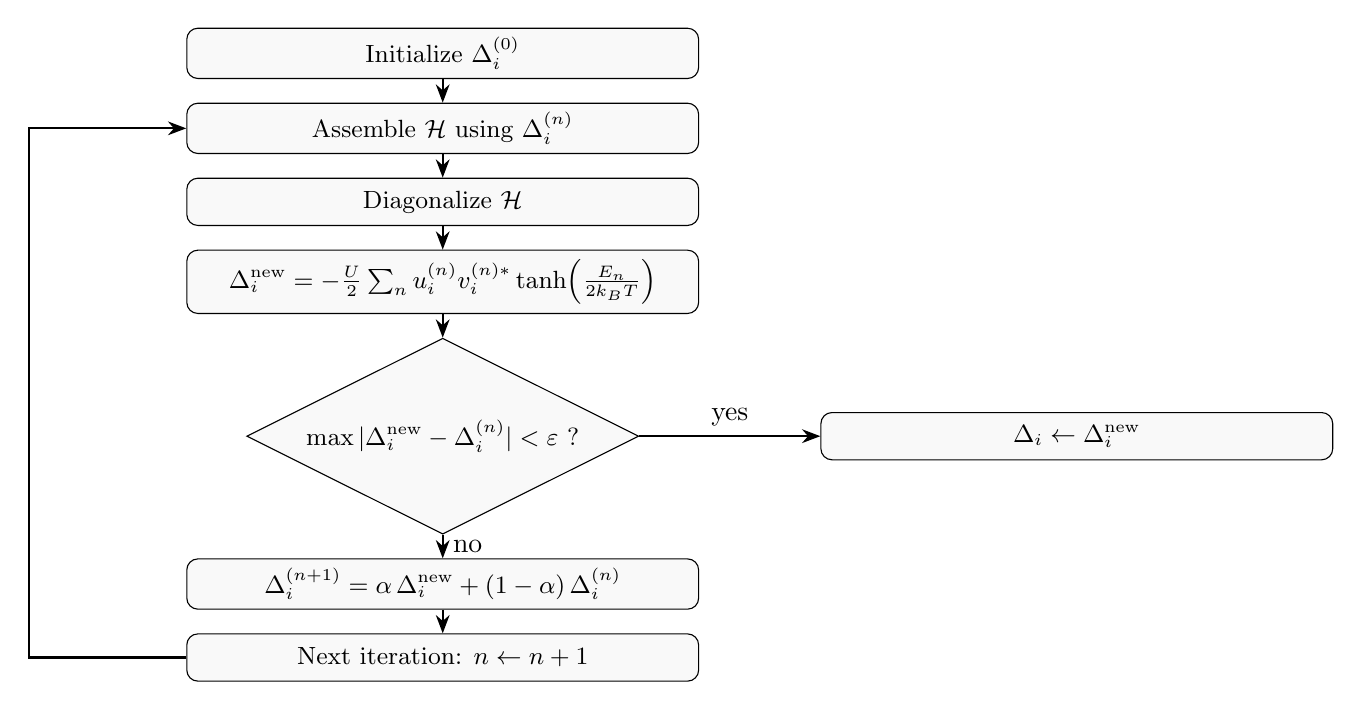
\begin{tikzpicture}[
    node distance=0.3cm,
    box/.style={
      rectangle, draw=black, fill=gray!5, rounded corners,
      minimum width=6.5cm, minimum height=0.6cm, align=center, font=\small
    },
    decision/.style={
      diamond, draw=black, fill=gray!5,
      minimum width=4.5cm, minimum height=0.5cm, align=center, font=\small, aspect=2
    },
    arrow/.style={thick, ->, >=Stealth}
  ]

% Nodes
\node[box] (init) {Initialize $\Delta_i^{(0)}$};
\node[box, below=of init] (assemble) {Assemble $\mathcal{H}$ using $\Delta_i^{(n)}$};
\node[box, below=of assemble] (diag) {Diagonalize $\mathcal{H}$};
\node[box, below=of diag] (newgap) {$\Delta_i^{\text{new}} = -\frac{U}{2}\sum_n u_i^{(n)}v_i^{(n)*}\tanh(\frac{E_n}{2k_BT})$};
\node[decision, below=of newgap] (converge) {$\max|\Delta_i^{\text{new}}-\Delta_i^{(n)}|<\varepsilon$ ?};
\node[box, right=of converge, xshift=2cm] (done) {$\Delta_i \leftarrow \Delta_i^{\text{new}}$};
\node[box, below=of converge] (mix) {$\Delta_i^{(n+1)} = \alpha\,\Delta_i^{\text{new}} + (1-\alpha)\,\Delta_i^{(n)}$};
\node[box, below=of mix] (loop) {Next iteration: $n\leftarrow n+1$};

% Arrows
\draw[arrow] (init) -- (assemble);
\draw[arrow] (assemble) -- (diag);
\draw[arrow] (diag) -- (newgap);
\draw[arrow] (newgap) -- (converge);
\draw[arrow] (converge) -- node[above] {yes} (done);
\draw[arrow] (converge) -- node[right] {no} (mix);
\draw[arrow] (mix) -- (loop);
% Loop back
\draw[arrow] (loop.west) -- ++(-2cm,0) |- (assemble.west);

\end{tikzpicture}
\caption{Self-consistent iteration algorithm.}
\label{fig:flowchart}
\end{figure}




\nocite{MilaHerviouSSP3,TimmSuperconductivity,zhu_bogoliubov-gennes_2016}

\printbibliography

\end{document}
